\chapter[Hadron production in pion-carbon interactions]{Hadron production in pion-carbon interactions}
\label{sec:hadron}

\note{TO REVIEW}

In this chapter we present the analysis of hadron production
in $\pi^-$-C interactions measured by the \NASixtyOne experiment
at CERN SPS. In~\cref{sec:showers:phen:had} we have stressed the
importance of $\pi^{\pm}$-air interactions for the air
shower development and, in particular, for the muon production.
The carbon target was selected here because of its similarity with
air nuclei in terms of nuclear mass. 

Our goal is to measure the production spectra of
\pions, \kaons, \protons, \lambs and \kzeros.
Althought our measurements of the \protons spectra
can impact directly the current understanding of the
air shower physics, all the particle spectra measured here
will be surely valuable for the testing of the hadronic
interaction models and for the tunning of the their next generation.
Besides that, the \lambs and \kzeros spectra have also an
important role on reducing the systematic uncertainties on the
\protons one.

The unprecedent $\pi^-$-C data analyzed here was
taken by the \NASixtyOne detector at two beam energies,
158 and 350 \GeVc. Its large acceptance that covers
a large region of the forward phase space makes the \NASixtyOne
the ideal detector for this kind of study. A previous
analyze of the $\pi^-$-C data with the measurements of
resonance mesons was published in Ref.~\cite{\RhoPaper}.
In particular, the measured $\rho^0$ spectra
also has a great impact on air shower physics.


The analysis presented in this chapter can be essentially
split in two parts. One of them is dedicated to the
measurements of the \pions, \kaons and \protons spectra
and the other to the \lambs and \kzeros spectra. The former
will be labelled along the text as the \emph{charged hadron analysis}
and its most challenging step includes the particle identification
through the measurements of the deposit energy of the particles.
On the other hand, the analysis of the latter group of particles
will be labelled by \emph{\vzero analysis},
being the signal extraction based on \minv spectra the
most challenging step. Although the two analysis
were in practice done separately, the analysis steps
that are conceptually the same will be presented here only once.

The charged hadron analysis was already in development
at the time this work started. The previous stages of the
analysis can be seen in Refs.~\cite{\IoanaICRC,\MichaelICRC,\HansICRC,\AlexICRC}.
Particularly, the event and track selection used here was based on
previous works of Martin Ruprecht~\cite{MartinThesis} and 
the \dedx fit strategy was based on previous works of Hans Dembinski.   
Concerning the \vzero analysis, there was no previous development
and the role analysis was done by the author of this thesis,
in collaboration with Michael Unger. 
A preliminary stage of the present analysis was published
in Ref.\cite{\RaulICRC}. 

%%%%%%%%%%%%%%%%%%%%%%%%%%%%%%%%%%%%%%%%
\section{\NASixtyOne experiment}
\label{sec:hadron:na61}

\note{TO REVIEW}

\warning{more references}

The \NASixtyOne~\cite{\NASixtyOnePaper} is a fixed target experiment located in the
North Area of the CERN SPS. Its proposal was accepted in 2006,
a pilot run took place in 2007 and the first physics run in 2009.
Most of its detector components were inherited from the
\NAFortyNine experiment~\cite{\NAFortyNinePaper},
which was shut down in 2003.

The physics programme of \NASixtyOne is very rich, including
heavy ion, neutrino and cosmic ray physics.
All these different fields have in commom the need for
precise hadron production measurements, which can be
provided by \NASixtyOne experiment. The main goals of the
heavy ion programme is the study of the properties of the
onset of deconfinement (discovered by \NAFortyNine~\cite{}) and
the search for the critical point of strongly interacting matter~\cite{}.
Concerning the neutrino physics programme, the hadron production
spectra in hadron-nucleus collisions measured by \NASixtyOne are
required to improve the neutrino flux predictions for the T2K experiment~\cite{\T2KPaper}.
Finally, the goal of the cosmic rays physics programme is to study
the properties of the $\pi$-C interactions, which is of highly value
for the better understanding of the extensive air shower physics and,
in particular, the muon production (see~\cref{sec:showers} for more details).


Its large acceptance is the main experimental feature of the
\NASixtyOne detector. A set of five Time Projection Chambers (TPCs)
can provide a high efficiency charged particle tracking.
A magnetic field partially covering the TPCs allows the reconstruction
of the particle momenta and charge while the energy loss measurements by the
TPCs allows for the particle identification. In~\cref{fig:hadron:na61:beam}
we show the configuration of the beam detectors as set for the $\pi^-$-C data taken
and in~\cref{fig:hadron:na61:setup} we show the configuration
of the main part of the \NASixtyOne detector. 
The coordenate system used in all \NASixtyOne analysis
is also shown in~\cref{fig:hadron:na61:setup}. The axis defined
by the beam direction is represented by the z coordenate,
while the x-y plane is the perpendicular to this direction.


A brief description of the beam and the detector
components relevant for the present analysis follows
in the next sections. Some important components,
like the Time-of-Flight detectors,
are not described here for the sake of briefity.
A detailed description of the experiment is given
in Ref.~\cite{\NASixtyOnePaper}.

%%%%%%%%%%%%%% BEAM %%%%%%%%%%%%%%%
\begin{figure}[!ht]
  \centering
  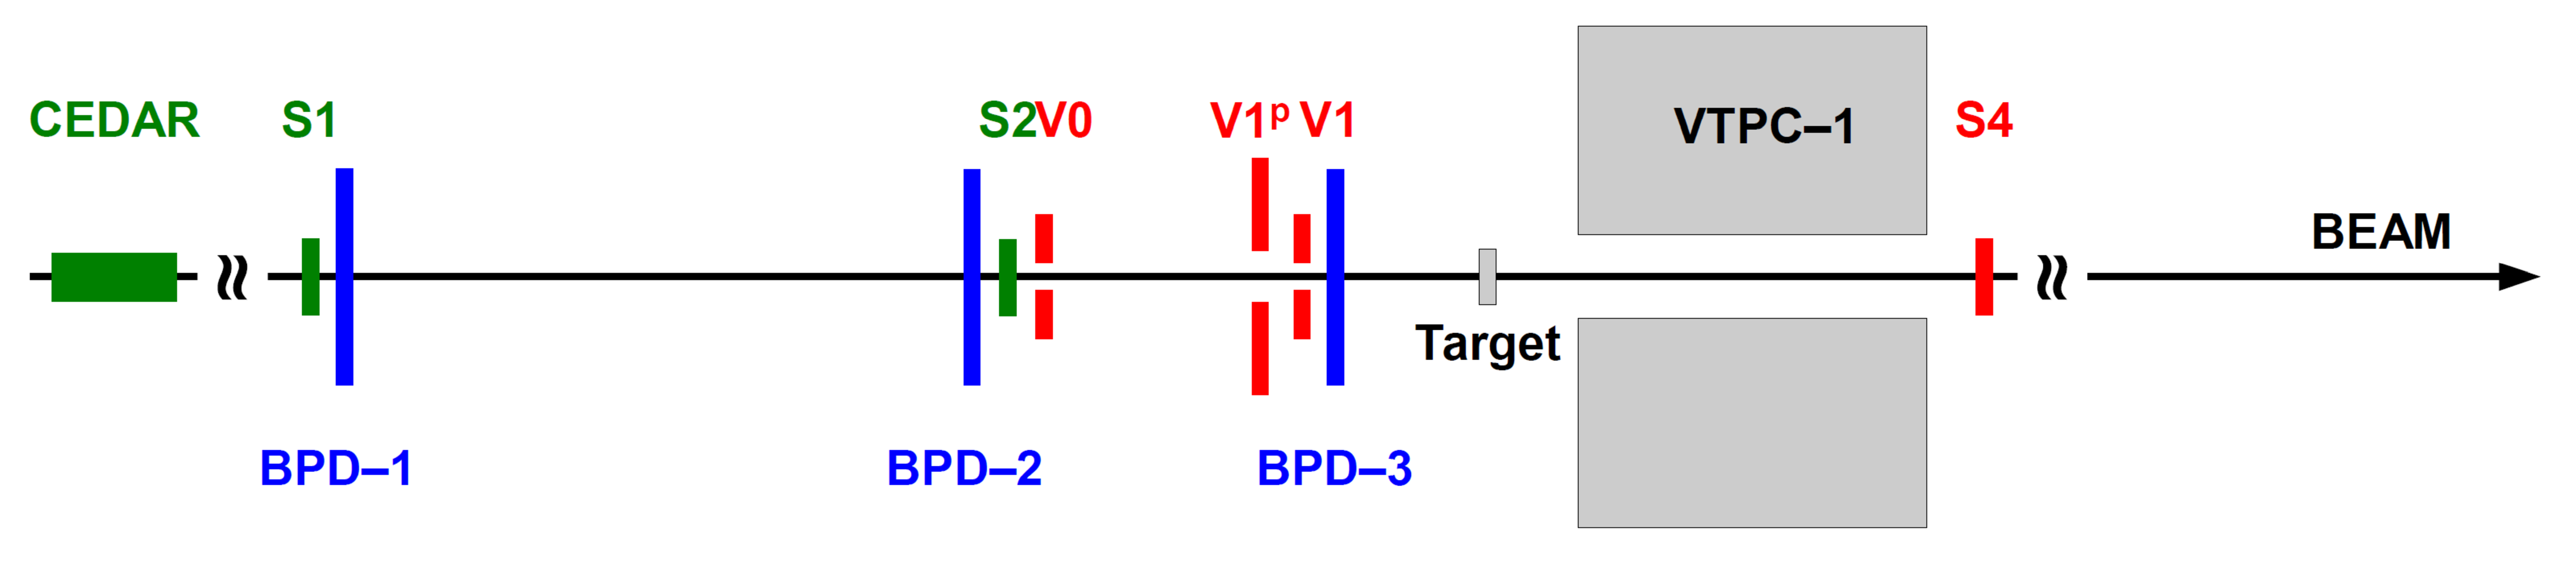
\includegraphics[clip, rviewport=0 0 1 1,width=0.95\textwidth]{det/Beam}
  \caption{}
  \label{fig:hadron:na61:beam}
\end{figure}



%%%%%%%%%%%%%% NA61 SETUP %%%%%%%%%%%%%%%
\begin{figure}[!ht]
  \centering
  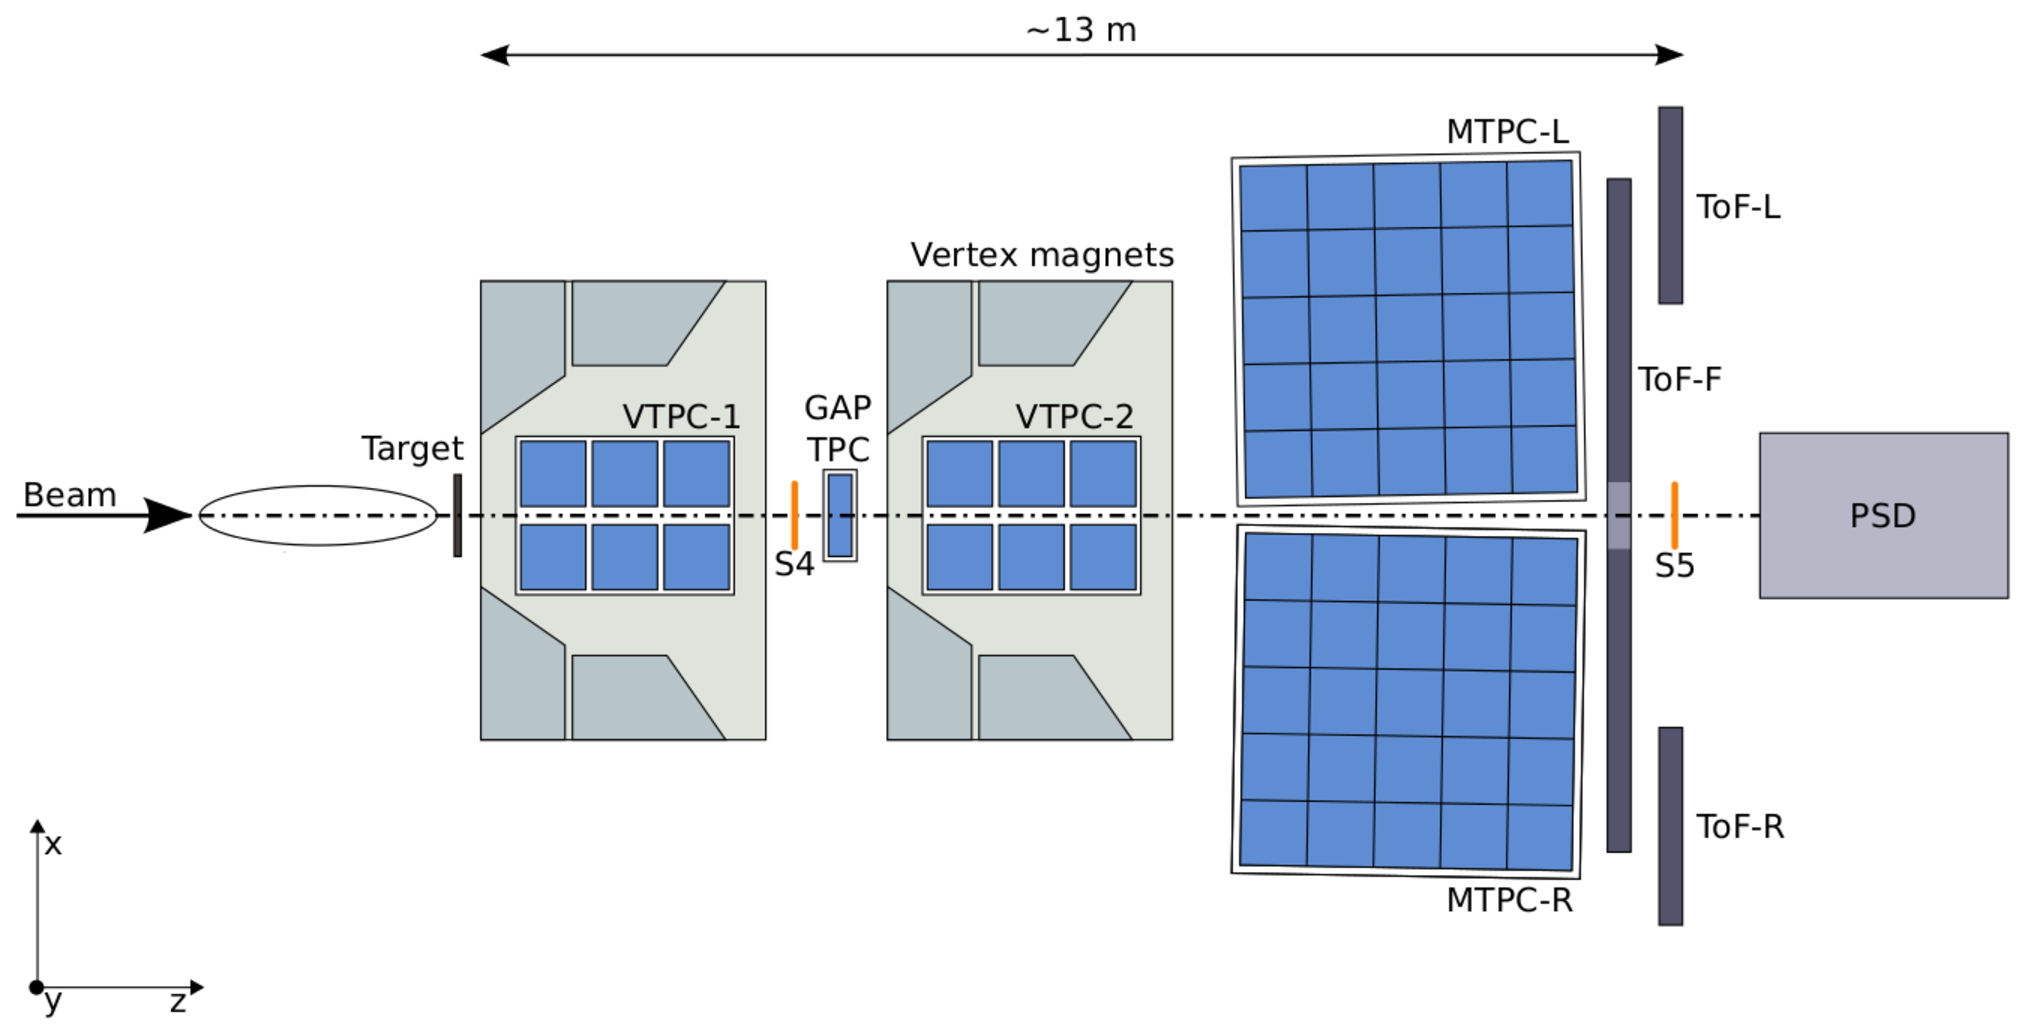
\includegraphics[clip, rviewport=0 0 1 1,width=0.95\textwidth]{det/na61}
  \caption{}
  \label{fig:hadron:na61:setup}
\end{figure}

%%%---------------------------------%%%
\subsection{Beam}
\label{sec:hadron:na61:beam}

The CERN SPS is able to provide to the North Area experiments
primary proton or ion beams of maximum energy of 450 \GeV/u. 
To generate the $\pi^-$ secondary beam, a primary proton
beam of 400 \GeVc from SPS is first collided against
a 10 cm long beryllium target. This collision occur
about 500 m upstream the \NASixtyOne detector.

The secondary charged particles produced are then tranported
through the H2 beamline. During the transportation,
a number of collimators and magnets are responsible for
selecting the momentum of the beam particles as well as
controlling their intensity and trajectory. For the data
analyzed in this work, the $\pi^-$ beam was generated
with two beam momenta, 158 and 350 \GeVc.


%%%---------------------------------%%%
\subsection{Beam detectors and trigger system}
\label{sec:hadron:na61:trigger}

The beam detectors and the components of the trigger system are shown
in~\cref{fig:hadron:na61:beam}. Most of them are placed upstream of
the target, being the S4 the only exception. A set of three plastic
scintillation counters are labelled as S1, S2 and S4. The components
V0, V1 and V1$^p$ are called veto detectors and they are also scintillation
counters but with a role in the beam trajectory. These veto detectors
are used in the trigger system in anti-coincidence so the beam particles
that pass away from the expected beam trajectory are removed.

Two trigger modes defined based on the scintillation counter measurements
are relevant for this work. The first one is the \emph{beam trigger},
denoted in this text as T1 and defined as 
$\text{S1}\wedge\text{S2}\wedge\overline{\text{V0}}\wedge\overline{\text{V1}}\wedge\overline{\text{V1}^p}$,
which means that S1 and S2 are considered in coincidence and V0, V1 and V1$^p$ in anti-coincidence.
The second relevant trigger is the \emph{interaction trigger}, denoted as T2
and defined as 
$\text{T1}\wedge\overline{\text{S4}}$.
The S4 detector in anti-coincidence removes events in which a beam
particle crossed the target without interacting. Evidently,
a small fraction of the inelastic interactions can produce
a high energy particle that reaches S4 and in these cases, the
event is not accepted. The consequent biased is taken into
account on the Monte Carlo correction step (see~\cref{sec:hadron:correction}).

The three Beam Position Detectors, indicated as BPD in~\cref{fig:hadron:na61:beam},
are proportional chambers that are able to measure the tranversal position
of the beam particles. Two important functions of the BPDs are to constrain
the tranversal position of the interaction vertex and to define the
incident angle of the beam particle on the target. Besides that,
the information about the spread of the beam particles on the
tranverse plane is used as a offline cut to assure the
selection of good quality events (see~\cref{sec:hadron:event}).

A further beam detector is the CEDAR, that is also shown
in~\cref{fig:hadron:na61:beam}. It is a Cherenkov detector
and its functionality is to identify the beam particle.
After the secondary beam particles are selected and
transported to the \NASixtyOne detector, the purity of the
$\pi^-$ beam is about 95\% and 100\% for the 158 and 350 \GeVc
case, respectively. The CEDAR information is also used as
an offline cut to assure that the interacting particle
is indeed a $\pi^-$.



%%%---------------------------------%%%
\subsection{Time projection chambers}
\label{sec:hadron:na61:tpc}

In~\cref{fig:hadron:na61:setup} one can see the
position of the five TPCs, which form the main part
of the \NASixtyOne detector. 
Two of them are the vertex TPCs, called
VTPC-1 and VTPC-2. Placed in between VTPC-1 and VTPC-2
there is the GAP-VTPC (or only GTPC). The two remain ones
are the left and right components of the main TPCs, which
are called MTPC-L and MTPC-R. 

The VTPC-1 and VTPC-2 are located inside two superconducting
dipole magnet. The produced magnetic field
is responsible for bending the particle trajectories,
which allows us to measure the sign of the particle charge
as well as the its momentum. To optimize the geometrical
acceptance, the intensity of the magnetic field is set
depending on the beam energy. For the $\pi^-$-C data taken
at 158 and 350 \GeVc, the magnetic field was set to 1.5 and 1.1 T
in te first and second magnets, respectively.

All the TPCs are filled with a gas mixture of Ar/CO$_2$ in the proportion
of 90/10 for the VTPCs and GPTC and 95/5 for the MTPCs.
The particle tracking is possible by collecting the electrons
freed by the ionization of the gas atoms because of the passage
of the charged particle.
These electrons are drifted along the y direction under the influence
of the an eletric field and collected by a set of readout pads on the top
of the TPCs. The electrons collected in the pads are group in time
to form the so called clusters. While the position of the pads
gives the x and z coordenates of the cluster position, the y
coordenate is reconstructed by its drifting time. By combining the
position of many clusters measured along the TPCs, we can reconstruct
the trajectory of the charged particles. The combination of the clusters
associated to one particle is called track.

Besides the particle tracking, the TPCs can also measure its
ionization energy loss. These measurements are done by combining
the total charge of all the clusters that compose a track and
a unique value of \dedx is defined for each particle.
The \dedx measurements allow the main particle
identification procedure applied in \NASixtyOne analysis
and we give more details about that in~\cref{sec:hadron:dedx:meas}.
A technical description of the TPCs of the \NASixtyOne can be found
in Refs.~\cite{AntoniAThesis,\NASixtyOnePaper}.





%%%%%%%%%%%%%%%%%%%%%%%%%%%%%%%%%%%%%%%%
\section{Data and simulation sets}
\label{sec:hadron:data}

\note{DONE}

The $\pi^-$+C data were collected by \NASixtyOne in 2009 at two beam energies:
158 and 350 \GeV. The carbon target consisted of
an isotropic graphite plate with 2 cm thickness along the beam axis,
with density of $\rho = 1.84$ g/cm$^3$. The target position was set to
80 cm upstream of VTPC-1. To estimate the contribution of 
interactions that occur with the detector material, about 10\% of the data
were taken with the target removed. 
In~\cref{sec:hadron:spec} we describe the procedure used to subtract
the effect of the out of target interactions from the measured spectra.
The calibration of the $\pi^-$+C data followed the standard
\NASixtyOne procedure, described in Ref.~\cite{Abgrall:2008zz}.


The Monte Carlo simulation sets used in this analysis
were created by first generating the primary interactions
using hadronic interaction models and then by passing
the produced particles through a detailed
detector simulation based on \GeantThree \warning{???} package~\cite{Brun:1994aa}.
Three hadronic interaction models were used: \EposLong~\cite{\EposPaper},
\DPMJetLong~\cite{\DPMJetPaper} and \QGSJetLong~\cite{\QGSJetPaper}.
For each beam energy and hadronic interaction model,
a simulation set was produced with approximately the same number of events
as in data. Both data and simulations were reconstructed
by the standard \NASixtyOne reconstruction chain~\cite{Abgrall:2011ae}. 


%%%%%%%%%%%%%%%%%%%%%%%%%%%%%%%%%%%%%%%%
\section{Event selection}
\label{sec:hadron:event}

\note{DONE}

The event selection can be divided into upstream
and event cuts. The upstream cuts are based on the
beam detector measurements and, since these detectors are not
implemented in the Monte Carlo simulations, these cuts were applied
only to the data. The upstream cuts are:
\begin{enumerate}[label=(\roman*)]
\item the CEDAR cut to identify the beam particle type and then remove
  the contributions from non-pion particles;
\item the WFA cut that uses the time information from the S1 detector
  to exclude events in which a second beam particle was detected
  within a time interval shorter than 2 $\mu$s;
\item the BPD cut that uses the information from the three BPD detectors
  to assure a good quality measurements of the beam position at the
  target plan.
\end{enumerate}
More details about the upstream cuts can be found in Ref.~\cite{MartinThesis}.

The event cuts that were applied to both data and simulations are:
\begin{enumerate}[label=(\roman*)]
\item the trigger cut to select events of the T2 type
  (see~\cref{sec:hadron:na61:trigger} for the trigger definitions);
\item the main vertex cut to remove events in which the main vertex
  was not properly fitted in the event reconstruction; 
\item the main vertex z-position cut to remove events in which the z coordinate of the fitted
  main vertex is farer than 17 cm from the main vertex position measured
  by the BPD detectors. \label{item:hadron:vtx}
\end{enumerate}
The main vertex z-position cut (\cref{item:hadron:vtx})
was applied to reduce the contribution of interactions
that occur out of the target. Because of the resolution
on the fitted main vertex z position, a small fraction
of interaction which occured in the target are also removed
by this cut. This bias effect is estimated and corrected in the
Monte Carlo correction step (see~\cref{sec:hadron:correction}).
In~\cref{tab:hadron:stat} we show the number of events after
the event selection for the data and simulation sets.

\begin{table}
  \begin{center}
    \caption{Number of events after the event selection for the data and simulation sets
      and for both beam momenta, 158 and 350 \GeVc.}
    \label{tab:hadron:stat}
    \begin{tabular}{|l|c|c|} \hline
                                    & 158 \GeVc            & 350 \GeVc \\ \hline
      Data (target inserted)        & 2.78$\times10^6$     & 2.59$\times10^6$ \\
      Data (target removed)         & 6.80$\times10^3$     & 6.12$\times10^3$ \\
      \EposLong                     & 3.59$\times10^6$     & 3.04$\times10^6$ \\
      \DPMJetLong                   & 3.89$\times10^6$     & 3.46$\times10^6$ \\
      \QGSJetLong                   & 3.56$\times10^6$     & 2.95$\times10^6$ \\ \hline
    \end{tabular}
  \end{center}
\end{table}

%%%%%%%%%%%%%%%%%%%%%%%%%%%%%%%%%%%%%%%%
\section{Phase space binning}
\label{sec:hadron:binning}

\note{DONE}

Both charged hadron and \vzero analysis were performed
by splitting the data into 2-dimensional phase space bins
of the \pp and \pT variables. For the
charged hadron analysis an unique phase space
binning was defined. The \pp intervals 
are nearly uniform in $\log p$. Only small adjustments
were done to move the crossing points of the energy deposit function
of different particles closer to the center of the bins.
Since some of these bins in the crossing regions
will be removed from the analysis (see~\cref{sec:hadron:dedx:sde}),
this strategy has shown effective to reduce the number of
removed bins. The average width of the \pp intervals is
$\Delta\log\pp=0.1$. Concerning the \pT intervals, the bin width
increases with \pT, being the width of the shorter and the longer ones
$\Delta \pT=0.1$ and  $\Delta\pT=0.5$, respectively.  
In~\cref{fig:hadron:binning:dedx} we show the
phase space binning used for the charged hadron analysis.


%%%%%%%%%%%%%% BINNING DEDX %%%%%%%%%%%%%%%
\begin{figure}[!ht]
  \centering
  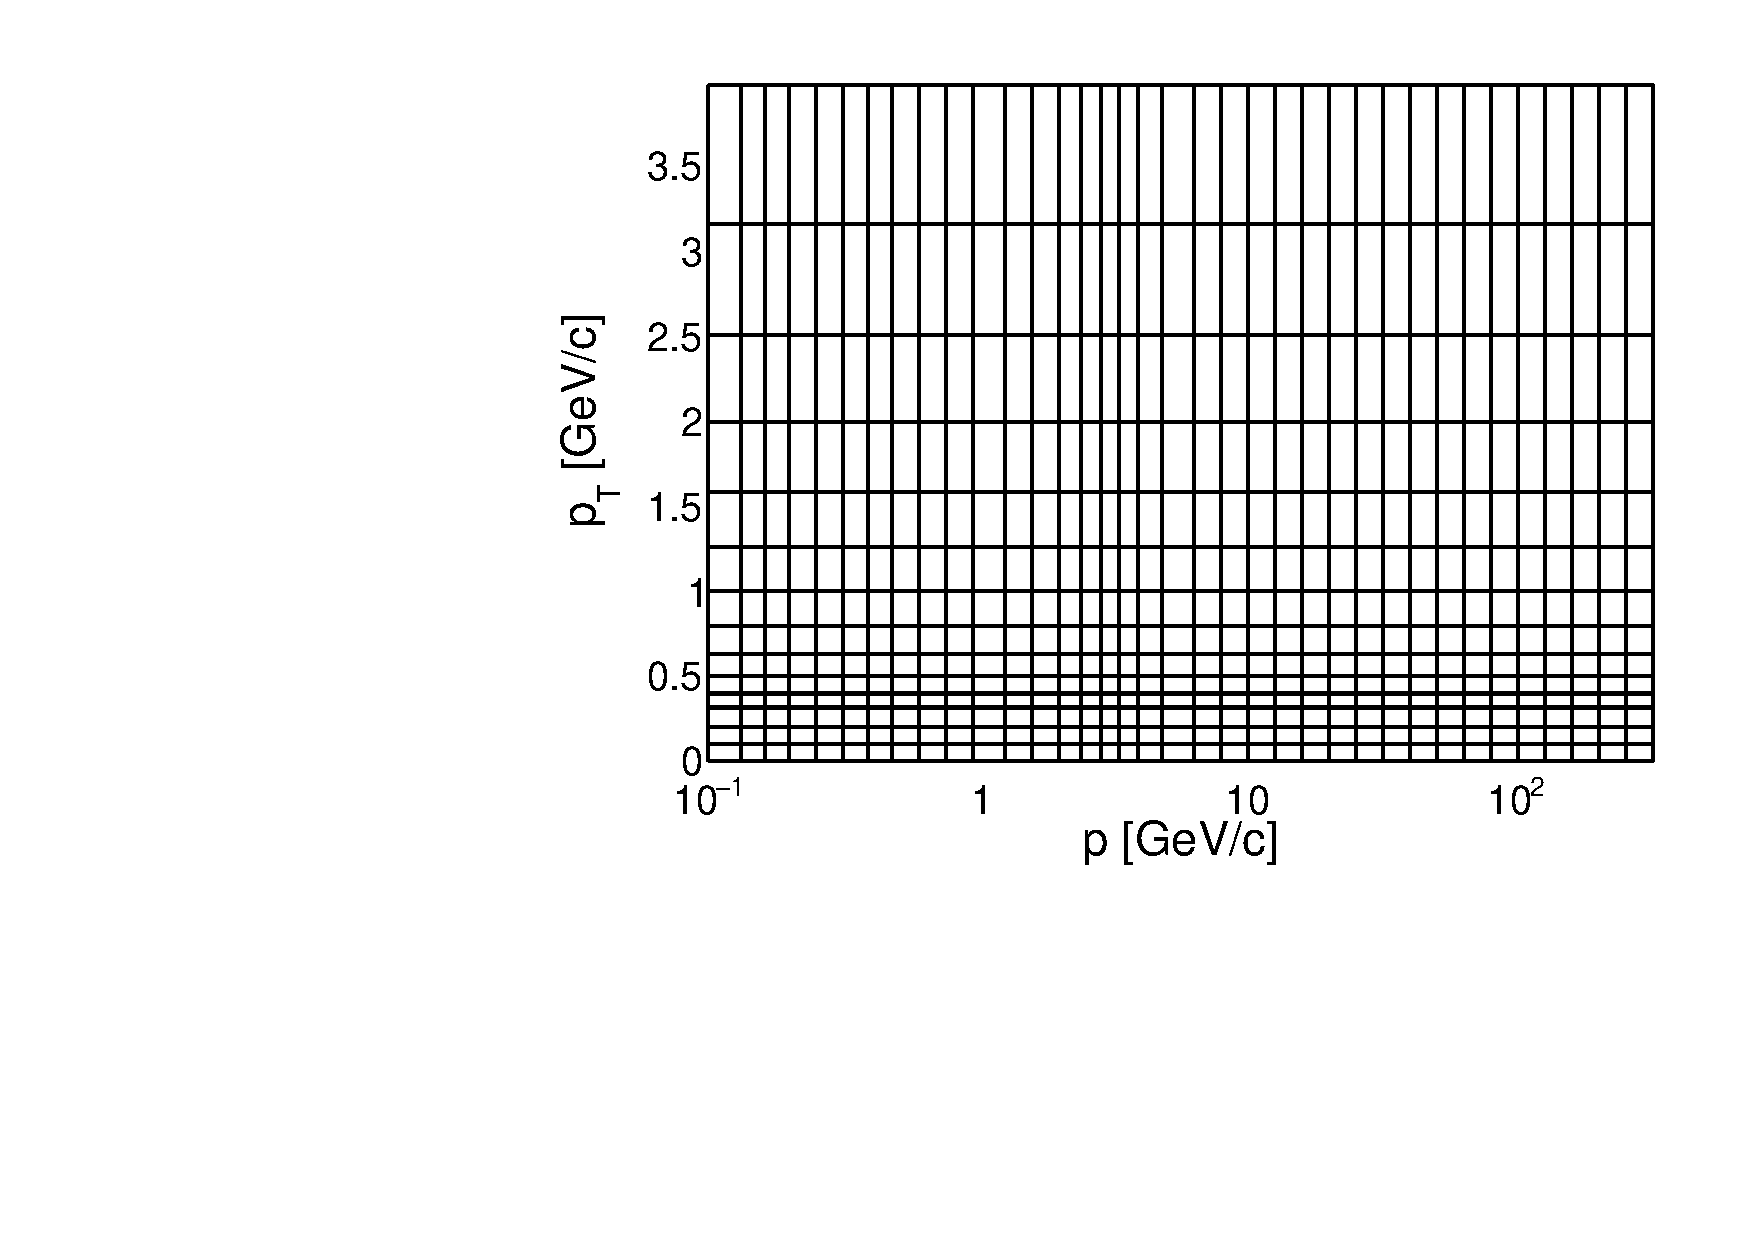
\includegraphics[clip, rviewport=0 0 1 1,width=0.5\textwidth]{DedxBinning}
  \caption{Illustration of the phase space binning used
    for the charged hadron analysis.}
  \label{fig:hadron:binning:dedx}
\end{figure}

Because the \vzero analysis is done independently for the three target particles,
the phase space binning is not required to be unique.
However, because the statistics is similar for \lamb and \antilamb,
the same binning was define for these two particles.
For either \lambs or \kzeros the \pp intervals vary from
$\Delta\log\pp=0.2$ to $0.3$. Concerning the \pT intervals,
the widths vary from $\Delta\pT = 0.2$ to $0.8$.
In~\cref{fig:hadron:binning:vzero} we show the 
binning used for the \vzero analysis.

%%%%%%%%%%%%%% BINNING V0 %%%%%%%%%%%%%%%
\begin{figure}[!ht]
  \centering
  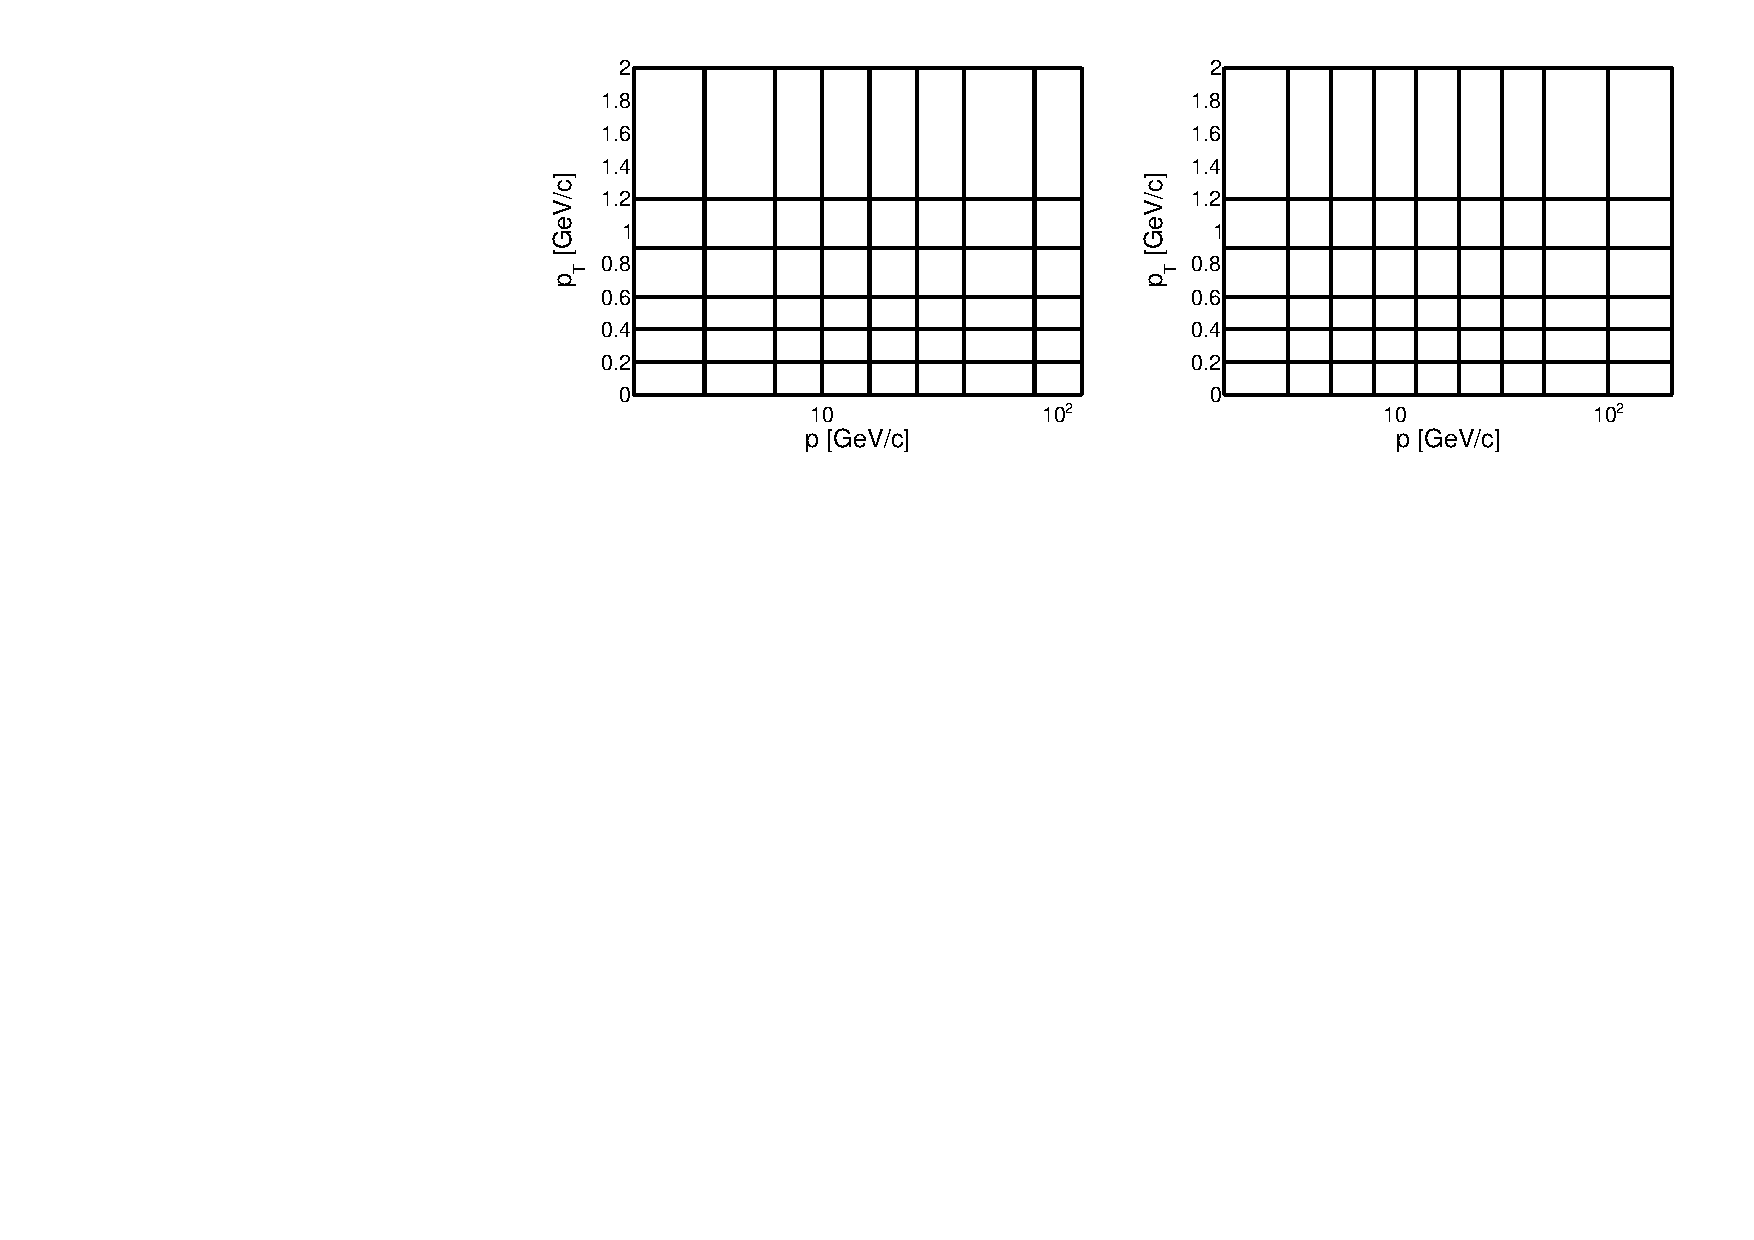
\includegraphics[clip, rviewport=0 0 1 1,width=0.8\textwidth]{V0Binning}
  \caption{Illustration of the phase space binning used
    for the \vzero analysis. The plot on the left show the binning
    used for \lamb and \antilamb and the plot on the right
    show the binning used for \kzeros.}
  \label{fig:hadron:binning:vzero}
\end{figure}


%%%%%%%%%%%%%%%%%%%%%%%%%%%%%%%%%%%%%%%%
\section{Particle identification for the charged hadron analysis}
\label{sec:hadron:dedx}

\note{DONE}

In this section we present the particle identification
analysis to obtain the spectra of \pions, \kaons and \protons.
This step is done in a track basis through the \dedx measurements,
being the aim here to determine the fraction of tracks which
correspond to each particle type on every phase space bin.
The track selection is first described in~\cref{sec:hadron:dedx:selection}
and a brief overview of the \dedx measurements is then given
in~\cref{sec:hadron:dedx:meas}.

The \dedx measurements only allow the particle identification
to be done statistically by fitting
the \dedx distributions with a combination of particle
types. Because of the complicated dependence of the \dedx
distributions on the particle momentum,
track properties (e.g. number of clusters) and
detector properties (e.g. resolution and calibration),
the \dedx fit turns to be a very challenging step.
The first requirement to perform it is the development
of an appropriate \dedx model, described in~\cref{sec:hadron:dedx:model}.

Having in hands the \dedx model, the measured \dedx
distributions can be fitted to determine the particle
fractions. However, the usual large number of
model parameters, added to the
overlap of the \dedx distributions
of different particles in certain phase space regions,
can make this fit very hard to perform.
Our fit strategy developed to overcome these difficulties is shown
in~\cref{sec:hadron:dedx:fit} and the results
of the fit in~\cref{sec:hadron:dedx:fitresults}. A new tool
developed in this work to evaluate the fit performance
and estimate bias and statistical uncertainties of the fit
is presented in~\cref{sec:hadron:dedx:sde}. This
tool is called Simulated Data Emsembles and
it is also used to define cuts on problematic
phase space bins and to compute correction factors.
Finally, in~\cref{sec:hadron:dedx:results} we show the results
of the particle identification analysis, including
the particle fractions of \pions, \kaons and \protons.


%%%%%%%%%%%%%%%%%%%%%%%%%%%%%%%%%%%%%%%%
\subsection{Track selection}
\label{sec:hadron:dedx:selection}

\note{DONE}

A set of selection criteria were
applied to the measured tracks aiming to
ensure the quality of their reconstruction. 
The list of selection criteria is the folowing.
\begin{enumerate}[label=(\roman*)]
\item The reconstructed track must be contained in the detector acceptance,
  that is defined based on two criteria. First,
  Monte Carlo simulations are used to define regions of the ($\phi$, \pp, \pT)
  phase space in which the selection efficiency is larger than 90\%. Second,
  the measured tracks are used to define regions of the same phase space in
  which the tracks hit directly the S4 detector~\cite{MartinThesis}. \label{item:track:acc} 
\item The total number of clusters on the track must be greater than or equal to 25.
\item The sum of clusters on both VTPCs must be greater than or equal to 12, or
  the number of cluster on the GTPC must be greater than of equal to 6.
\item The distance between the extrapolated track to the interaction plane and the
  interaction point must be smaller than 4 cm on the both horizontal and vertical plane.
\end{enumerate}

The acceptance selection (\cref{item:track:acc}) is important because
it was observed that the Monte Carlo simulations cannot describe
accurately the detector efficiency in the phase space regions
in which this efficiency is relatively low (<90\%). Since the detector
acceptance is the dominant effect to be corrected at the Monte Carlo
correction step, this discrepancy between data and simulations
could significantly bias the resultant spectra if the acceptance selection
was not applied.

After the track selection, the measured tracks were split
into two subsets called Right Side Tracks (RST) and Wrong Side Tracks (WST).
The former group is defined as the tracks that bend away from the
beam axis, while the latter as the tracks that bend towards the beam axis.
Given the track $\phi$ angle and its charge $q$, the two groups
can be defined by the sign of the product $q \times \cos(\phi)$, where
RST have positive sign and WST have negative ones.
The distinction between this two track topologies is motivated by the
fact that a right and a wrong side track with the same \pp and
\pT cross different regions of the detector, 
which in turn have important implications on the
particle identification step based on the \dedx measurements
(see~\cref{sec:hadron:dedx}). 
In~\cref{fig:hadron:track:topologies} we ilustrate the
RST and WST definitions.

%%%%%%%%%%%%%% RST/WST %%%%%%%%%%%%%%%
\begin{figure}[!ht]
  \centering
  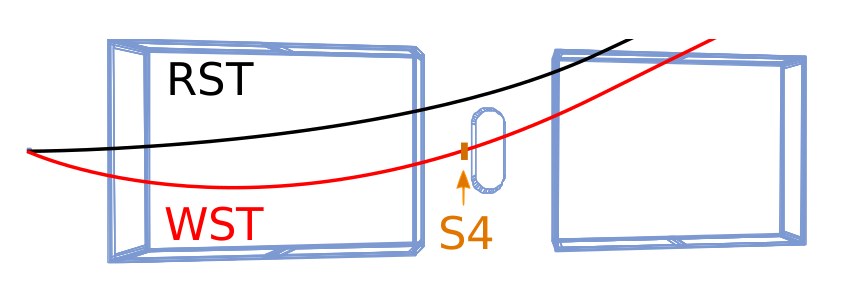
\includegraphics[clip, rviewport=0 0 1 1,width=0.95\textwidth]{track_topologies}
  \caption{\warning{DO IT} \cite{MartinThesis}}
  \label{fig:hadron:track:topologies}
\end{figure}


%%%---------------------------------%%%%
\subsection{\dedx measurements}
\label{sec:hadron:dedx:meas}

\note{DONE}

The \dedx is defined as the energy lost by the
particle to the medium per unit of length. 
In \NASixtyOne, the \dedx is measured by the TPCs, which collect the 
freed electrons from the ionization of the gas by the passage of the charged particles.
The determination of the \dedx from the signal recorded at the TPCs requires a complex and
detailed procedure that has been very well established by the \NAFortyNine and \NASixtyOne
experiment along the last decades. Since the detailed description 
is out of the scope of this text, only the general idea and the most important aspects
will be presented in the next paragraphs. More complete and detailed approaches
can be found in Refs.\cite{BlumBook,LeeuwenThesis,GaborVeresThesis}.

Several processes can contribute to the energy loss of charged particle due to
its interaction with atoms of the gas in the TPCs, being the emission of
electrons by ionization the most relevant one. The electrons emitted are
drifted through the chamber and collected in the readout pads, which records
the signal as ADC charges. A cluster is defined as a set of consecutive charges.
The total charge measured for each cluster is related to the \dedx of each track.
However, numerous detector effects have to be corrected at the cluster level before
grouping the clusters in one unique \dedx value. The simplest correction accounts for
the geometrical differences due to the particle incident angle in the pad and
the pad widths. More complicated corrections account for differences in the electronic
gain and gas pressure/temperature of the pads, differences in the sector gains and
losses of electrons during the drift in the chambers and in the readout pad.
A detailed description of the correction procedure can be found in Ref.~\cite{AntoniMThesis}.

The track \dedx is then determined by the combination of the corrected 
charges from all track clusters. Because of the well known Landau-like shape of the
energy loss probability distribution, the average and the variance
of the measured charges are not well behaved for typical number of clusters
($\sim$ 20-150). This makes the simplest approach, by defining the track \dedx
as the average charge over all cluster, not suitable. 
To overcome this issue and to obtain a satisfactory \dedx resolution,
the method of the truncated mean is applied, in which only a subset of the clusters
is selected to compute the average. The selected clusters are defined by ordering
the values of the charge and then selecting the ones inside a given fractional interval.
For the \NASixtyOne experiment it was found the optimal interval being the 50\%
of the clusters with the smallest charges~\cite{GaborVeresThesis}.

It is important to point out that, although the \dedx associated to
a track is proportional to the energy lost by the particle,
these two quantities are not exactly the same. This
means that the measured \meandedx as a function of \pp
does not follow the expected Bethe-Bloch function, but it does
behave in a very similar way. Because of this similarity,
the functional form of the Bethe-Bloch function
is used here to parametrize the \meandedx evolution
with \pp. In~\cref{fig:hadron:dedx:bb} we show the distribution of
the measured \dedx as a function of the track \pp
together with the \meandedx parametrization for 
several particle types. This parametrization was developed
for this analysis and it is an important element for the \dedx model
and the \dedx fit presented in~\cref{sec:hadron:dedx:model,sec:hadron:dedx:fit}.


%%%%%%%%%%%%%% DEDX DATA %%%%%%%%%%%%%%%
\begin{figure}[!ht]
  \centering
  
  \begin{overpic}[clip, rviewport=0 0 1 1,width=0.47\textwidth]{dedx/Dedx_0_0}
    \put(18,60){(a)}
  \end{overpic}
  \begin{overpic}[clip, rviewport=0 0 1 1,width=0.47\textwidth]{dedx/Dedx_0_1}
    \put(18,60){(b)}
  \end{overpic}
  
  \begin{overpic}[clip, rviewport=0 0 1 1,width=0.47\textwidth]{dedx/Dedx_1_0}
    \put(18,60){(c)}
  \end{overpic}
  \begin{overpic}[clip, rviewport=0 0 1 1,width=0.47\textwidth]{dedx/Dedx_1_1}
    \put(18,60){(d)}
  \end{overpic}
  
  %\subfloat[][Positively charged particles from the 158 \GeVc data set.]
  %         {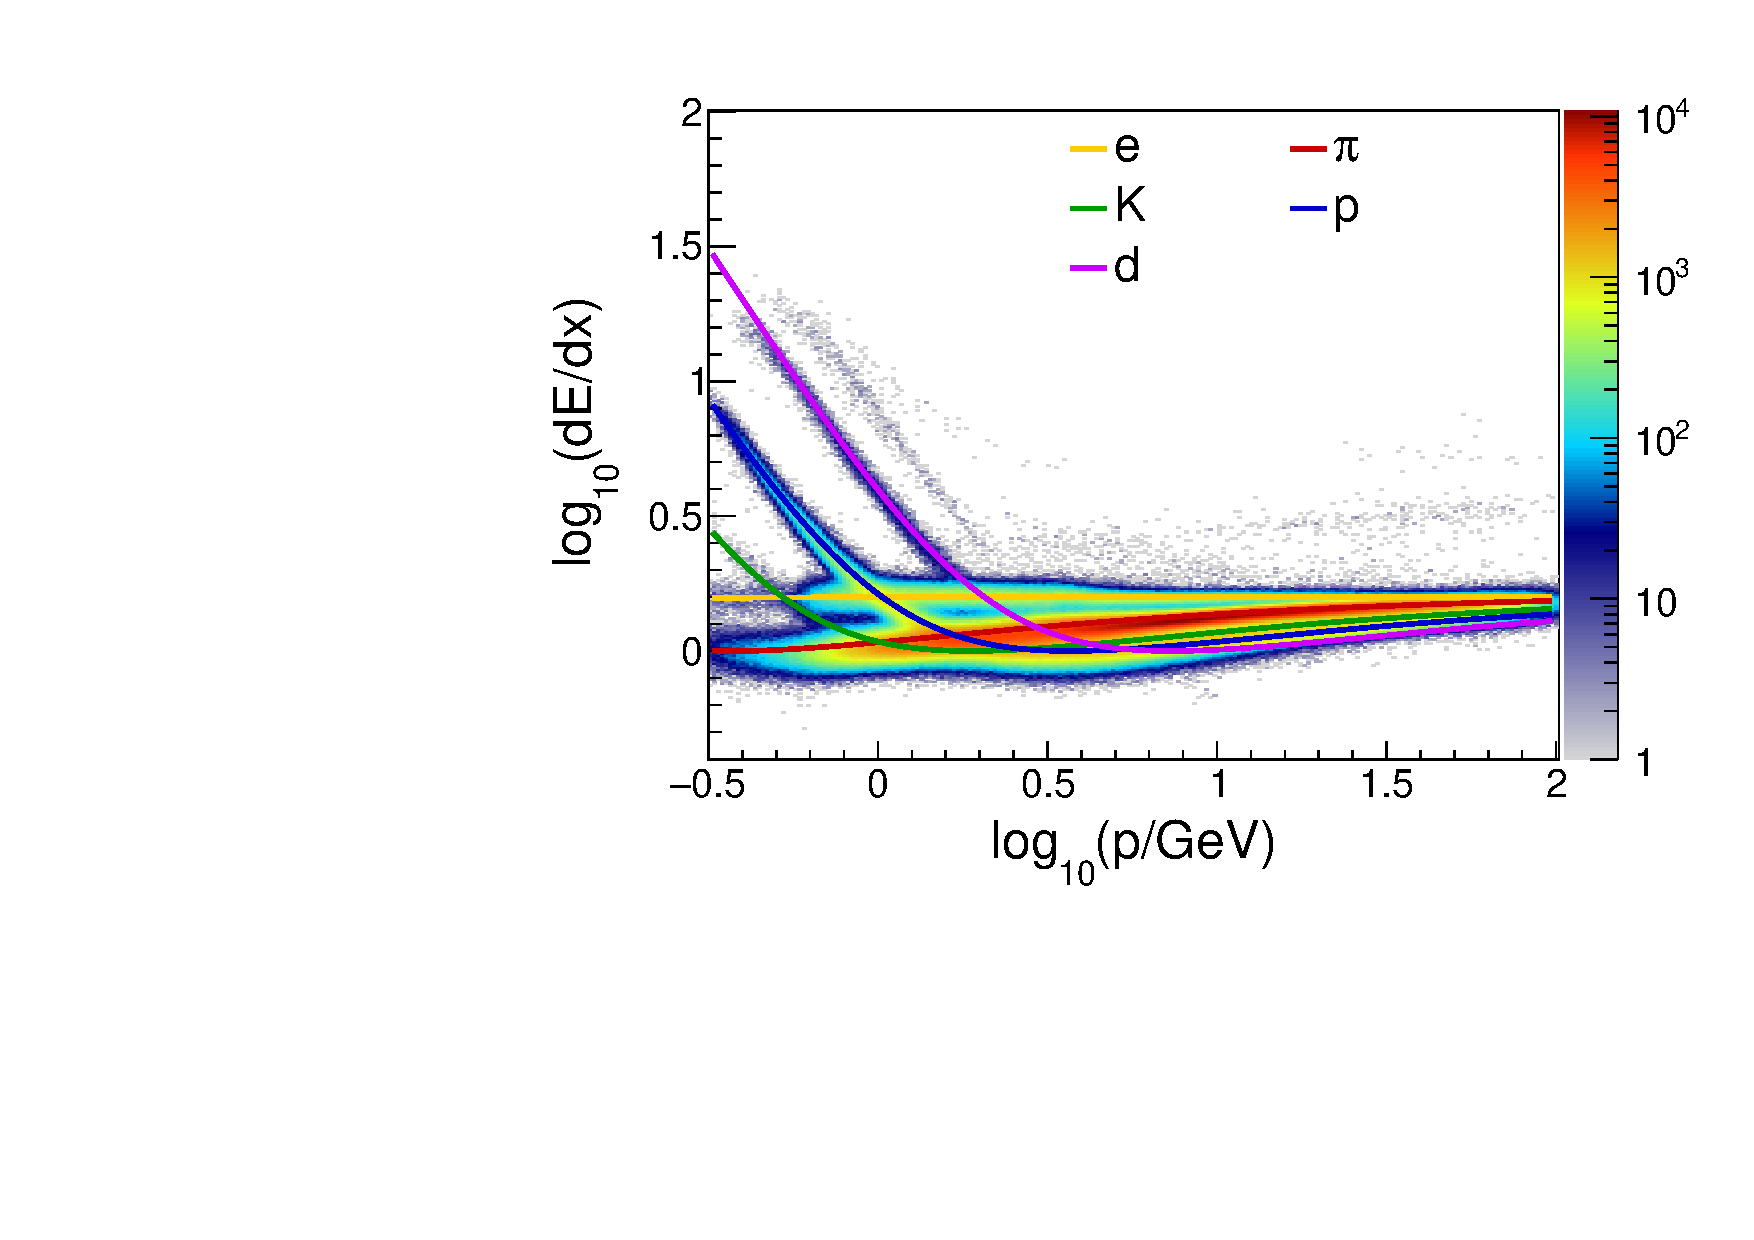
\includegraphics[clip, rviewport=0 0 1 1,width=0.47\textwidth]{dedx/Dedx_0_0}}
  %\subfloat[][Negatively charged particles from the 158 \GeVc data set.]
  %         {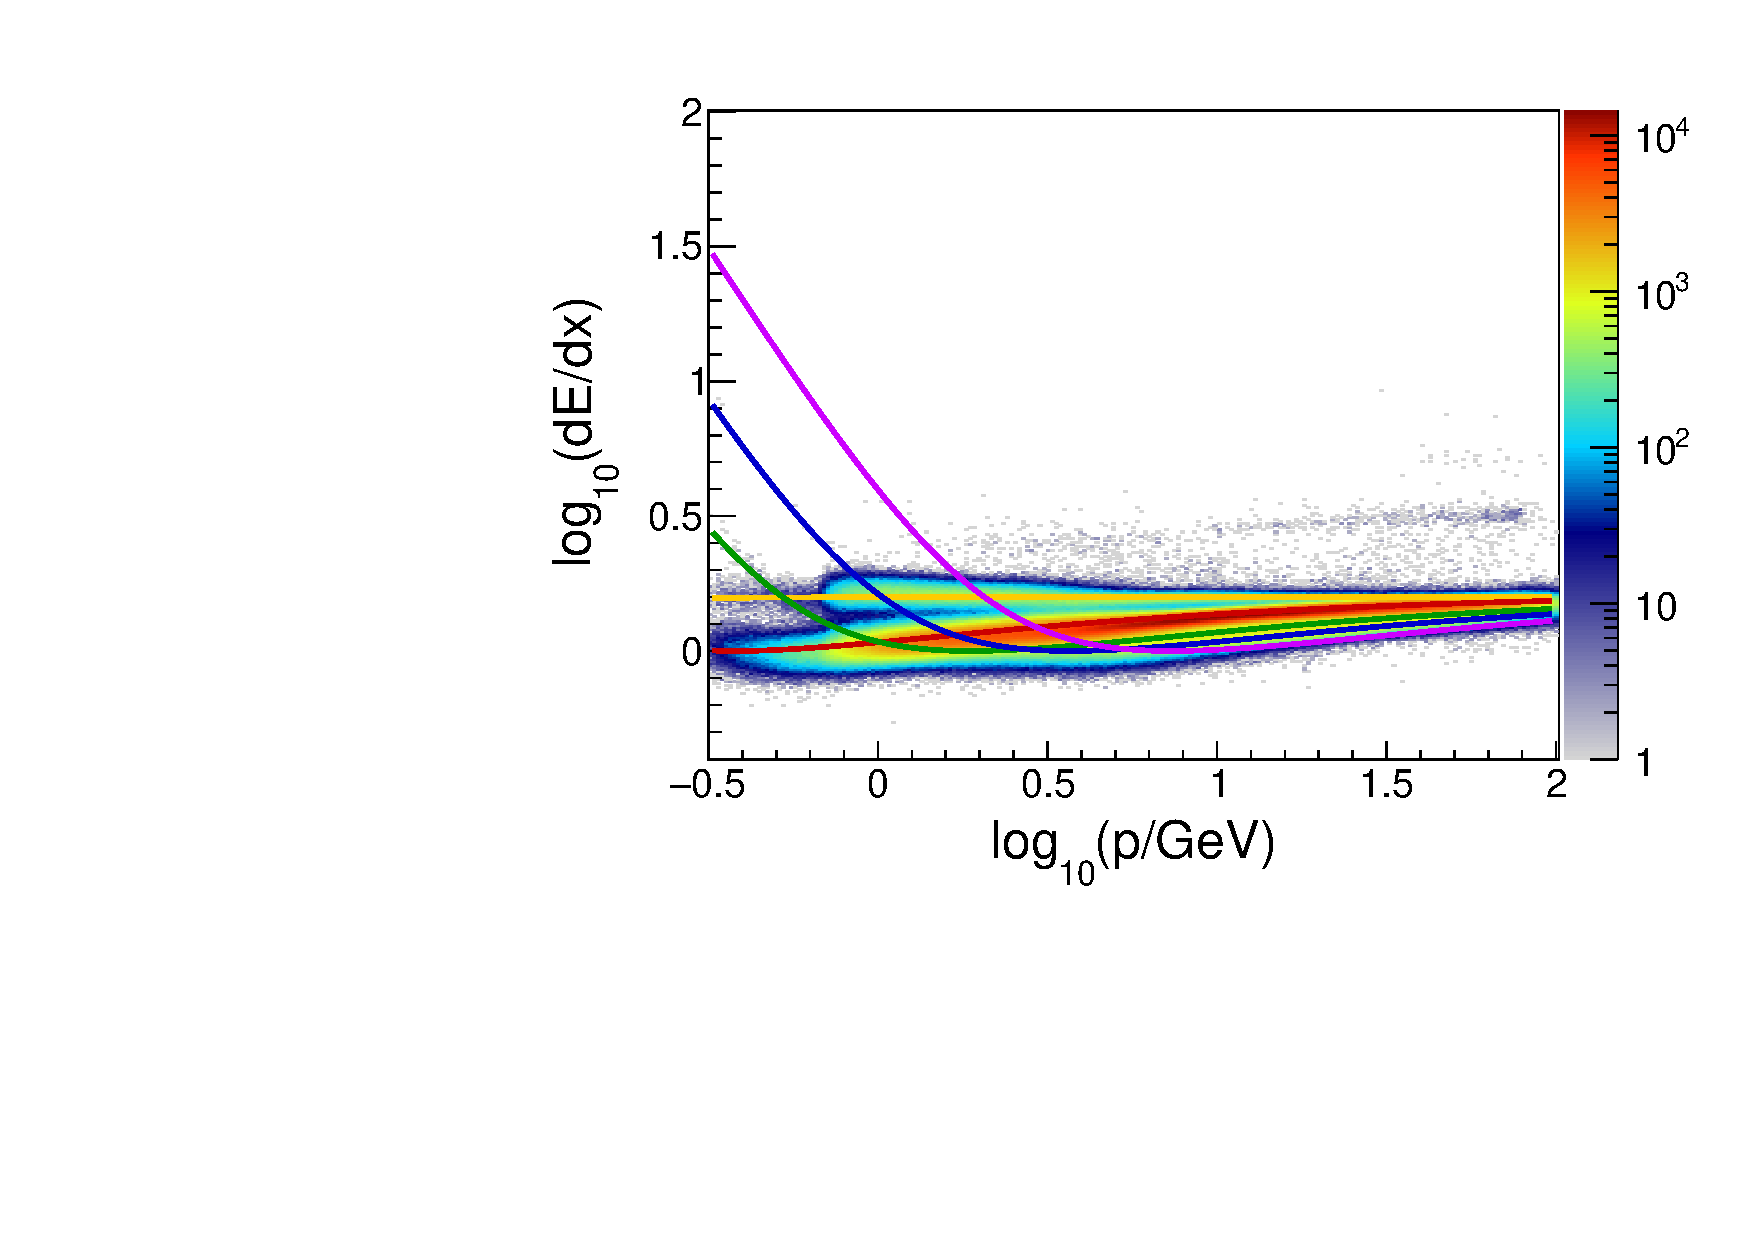
\includegraphics[clip, rviewport=0 0 1 1,width=0.47\textwidth]{dedx/Dedx_0_1}}
  %\subfloat[][Positively charged particles from the 350 \GeVc data set.]
  %         {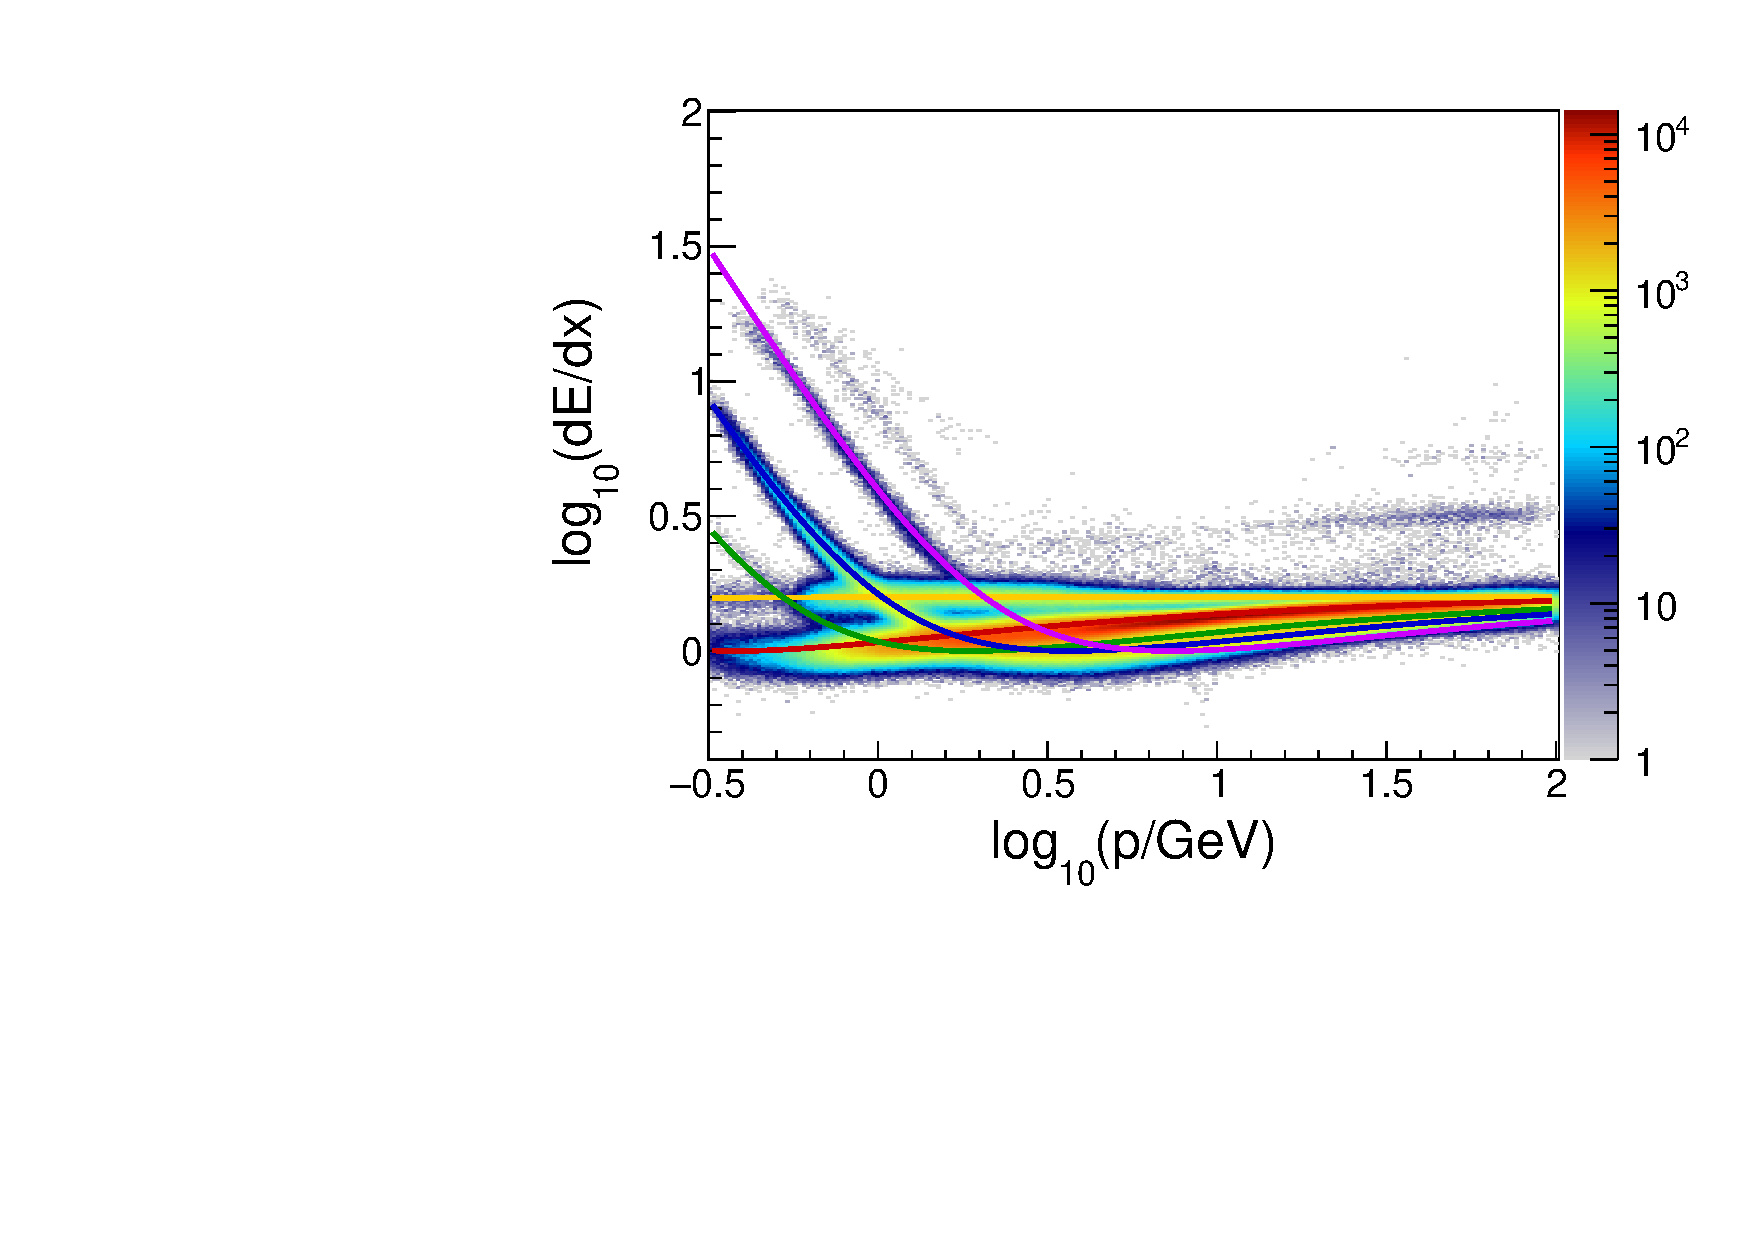
\includegraphics[clip, rviewport=0 0 1 1,width=0.47\textwidth]{dedx/Dedx_1_0}}
  %\subfloat[][Negatively charged particles from the 350 \GeVc data set.]
  %         {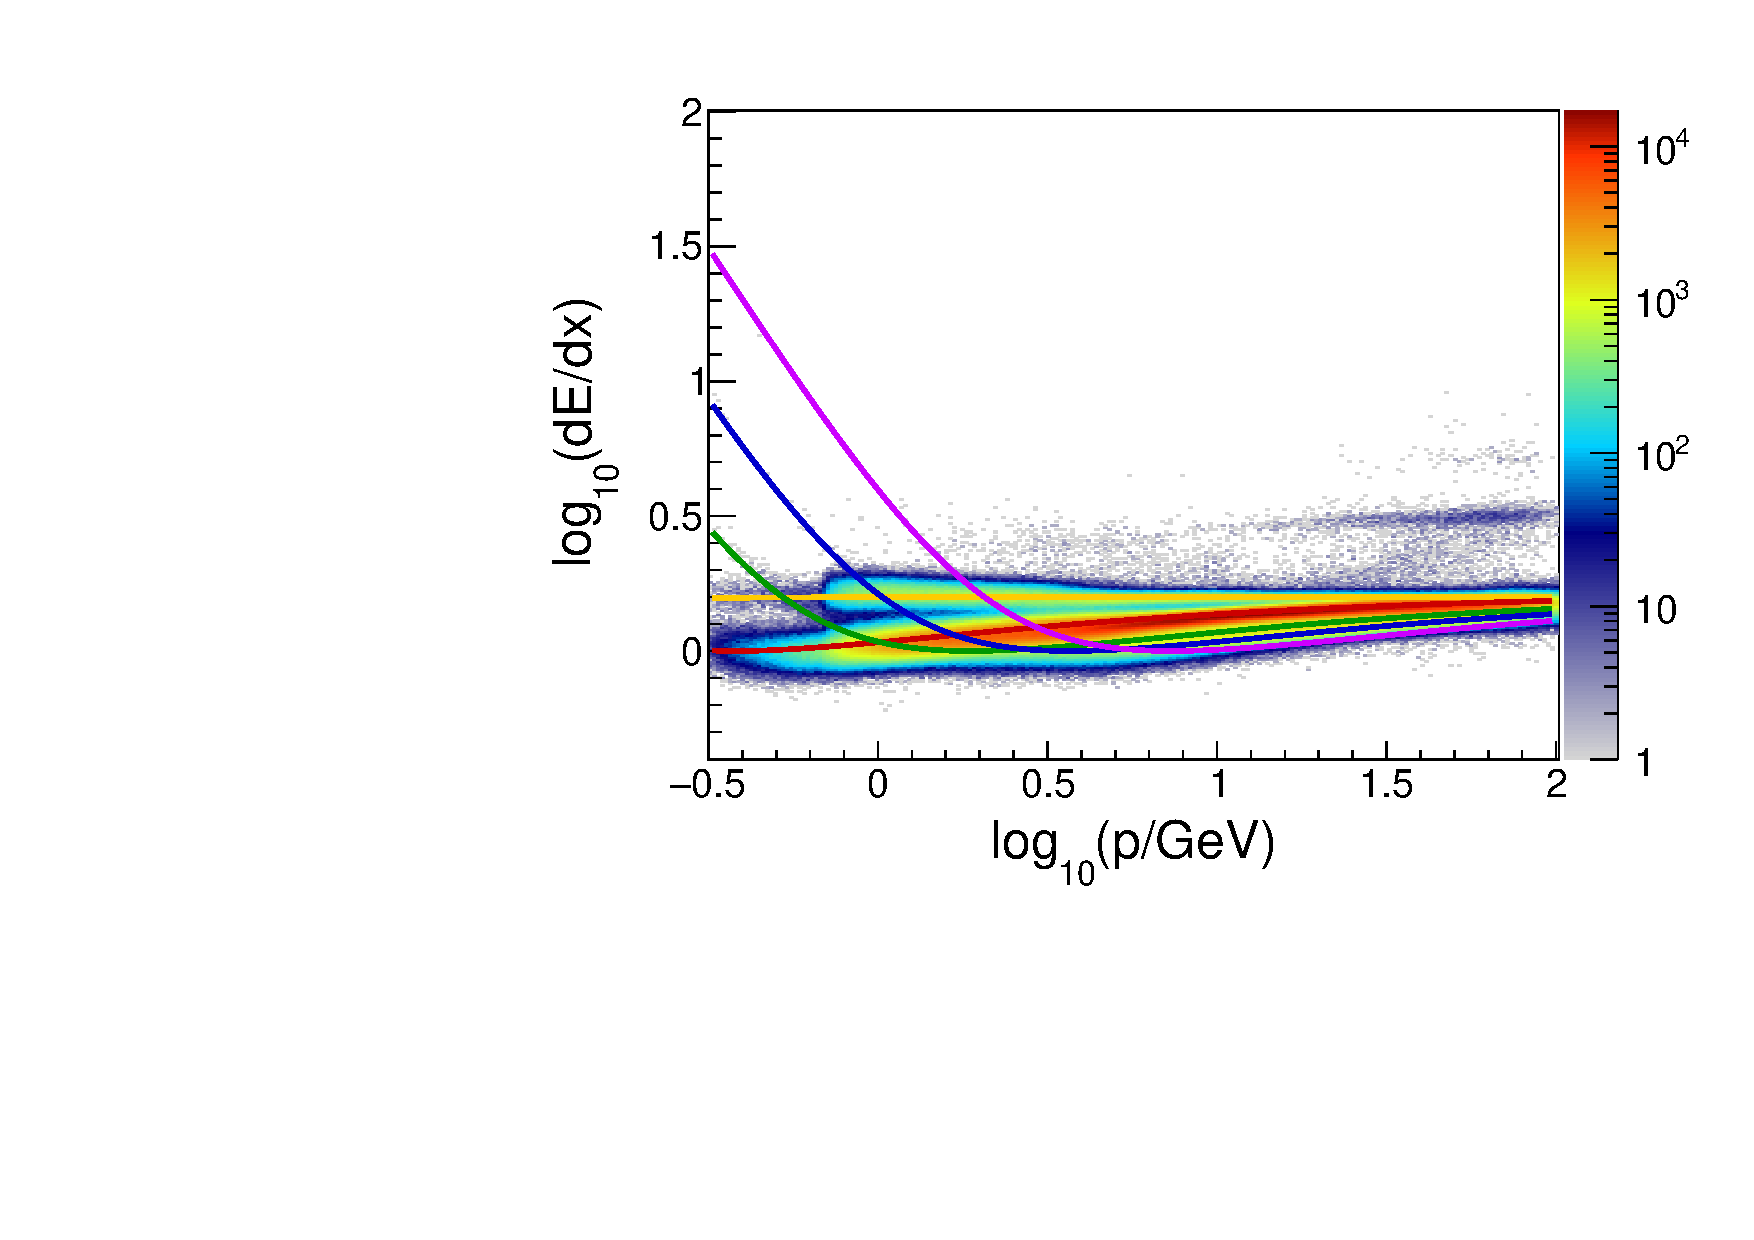
\includegraphics[clip, rviewport=0 0 1 1,width=0.47\textwidth]{dedx/Dedx_1_1}}
  
  \caption{\dedx data used in this analysis. Positively and negatively charged tracks
    are shown repectively in (a) and (b) for the 158 \GeVc data set,
    and in (c) and (d) for the 350 \GeVc one. The solid curves
    show the \meandedx parametrization for each particle type. \warning{noise rejection}}
  \label{fig:hadron:dedx:bb}
\end{figure}


%%%---------------------------------%%%%
\subsection{\dedx model}
\label{sec:hadron:dedx:model}

\note{DONE}

To perform the \dedx fit , a model to describe the \dedx distributions
of different particle types as a function of their
momenta is required. While experiments like
ALICE~\cite{\AlicePaper} and CMS~\cite{\CMSPaper} opt
for modeling the \dedx distributions
with templates~\cite{CorralesMorales:2017zty,Chatrchyan:2012qb},
the \NAFortyNine and \NASixtyOne experiments traditionally adopt
an analytic model, which will also be adopted by us.
Although the model chosen for our analysis is based on previous
studies from \NAFortyNine and \NASixtyOne
collaborations~\cite{LeeuwenThesis,GaborVeresThesis},
it contains particular features that we have found
to be the most suitable for the present analysis. 

For clarification, we first present the notation
adopted along this text. The particle types are represented by the index
\ipart, which can be one of the five particles $\ipart=e$, $\pi$, K, p or d.
The positive and negative charges are indexed by
\ich, so that $\ich = +$ or $-$. In addition, \ncl is used to
represent the number of cluster of a track and the \dedx
is replaced by \eps for shortening.

The first element of our \dedx model is the probability density
function of \eps for a given particle type and charge, which is called
here $f_{\ipart,\ich}(\eps)$.
Because \eps is obtained by averaging the measured charge
over a certain number of clusters, it is natural to assume 
that the shape of $f_{\ipart,\ich}(\eps)$ depends on \ncl.
To be more precise, the width of $f_{\ipart,\ich}(\eps)$
(or the \eps resolution) should decrease
with increasing \ncl, and vice-versa. 
Furthermore, the mean of $f_{\ipart,\ich}(\eps)$ is expected  
to evolve with the particle momentum \pp
by following a Bethe-Bloch-like function.
Given its \ncl and \pp dependences, $f$ can
be taken as a conditional probability function,
so it can be written as $f_{\ipart,\ich}(\eps|\pp,\ncl)$.

It has been verified that $f_{\ipart,\ich}(\eps|\pp,\ncl)$
can be well represented by an asymmetric
Gaussian function~\cite{GaborVeresThesis}. 
Thus, we can write
\begin{equation}
  f_{\ipart,\ich}(\eps|\pp,\ncl) = \frac{1}{\sqrt{2\pi}\sigma_{\ipart,\ich}} \;
  \exp\left[-\frac{1}{2}\left(\frac{\eps-\mu_{\ipart,\ich}}{\delta \; \sigma_{\ipart,\ich}}\right)^2\right],
  \label{eq:hadron:dedx:model:pdf}
\end{equation}
with
\begin{equation}
  \delta =
  \begin{cases}
    & 1-d, \ \ \ \eps \le \mu_{\ipart,\ich} \\
    & 1+d, \ \ \ \eps > \mu_{\ipart,\ich}, \\
  \end{cases}
  \label{eq:hadron:dedx:model:asymm}
\end{equation}
where $\mu$ is the mode of the distribution, $\sigma$ is its resolution
and $d$ is the asymmetry parameter. The \pp and \ncl dependence are implicit
on the parameters $\mu$ and $\sigma$, as will be explained next.
The mode $\mu$ is related to the mean of \eps (\meaneps) by
\begin{equation}
  \mu_{\ipart,\ich} = \meaneps_{\ipart,\ich} - \frac{\sigma_{\ipart,\ich}}{\sqrt{2\pi}}
  \left[\left(1+d\right)^2 - \left(1-d\right)^2 \right].
  \label{eq:hadron:dedx:model:mu}
\end{equation}

The Bethe-Bloch parametrizations shown as colored curves
in~\cref{fig:hadron:dedx:bb} give the \meaneps as a
function of \pp for a given particle type.
In this model, this parametrization is used for reference
and the value of \meaneps from the parametrization
is denoted by \meanepsbb.
To account for deviations from \meanepsbb,
our model includes a set of parameters called
\textit{calibration constants}, which are denoted by $X$.
These parameters act as logarithmic shifts of the \meaneps
around \meanepsbb and they can in principle be applied
to each particle and charge separately. However, to reduce the complexity
of the model, we assume one global calibration constant
for each charge that follows the \meaneps of the $\pi$ distribution
and individual calibration constants for the other particle types,
which are common for both charges. The \meaneps for a
given \ipart and \ich is then given by
\begin{equation}
  \meaneps_{\ipart,\ich} =
  \begin{cases}
    & \meaneps_{\ipart}^\text{BB} \; e^{X_{\ipart}^{\ich}} \ \ \ \ \ \ \ \ (i=\pi) \\
    & \meaneps_{\ipart}^\text{BB} \; e^{X_{\pi}^{\ich}} \; e^{X_{\ipart}^{\ich}} \ \ \ (i\neq\pi).
  \end{cases}
  \label{eq:hadron:dedx:model:cal}
\end{equation}
In total, the model includes 6 calibration constants:
$X_{\pi}^{+}$, $X_{\pi}^{-}$, $X_{e}$, $X_{K}$, $X_{p}$ and $X_{d}$.
The \meaneps from~\cref{eq:hadron:dedx:model:cal} is used
in~\cref{eq:hadron:dedx:model:mu} to compute $\mu_{\ipart,\ich}$,
which is in turn used in~\cref{eq:hadron:dedx:model:pdf}
to compute $f_{\ipart,\ich}(\eps|\pp,\ncl)$.

The last ingredient of~\cref{eq:hadron:dedx:model:pdf}
to be described is the resolution $\sigma_{\ipart,\ich}$. 
Its \ncl dependence is assumed to be of the form
$\sigma \sim 1/\sqrt{\ncl}$. Besides that $\sigma_{\ipart,\ich}$
is also assumed to depend on the \meaneps by a power law relation.
The overall scale of $\sigma_{\ipart,\ich}$ is given by its normalization
parameter $\sigma_0$, which is actually defined separately for each charge ($\sigma_0^{\ich}$).
The final expression for the resolution is,
\begin{equation}
  \sigma_{\ipart,\ich} = \frac{\sigma_0^{\ich}}{\sqrt{\ncl}} \meaneps_{\ipart,\ich}^{\alpha},
  \label{eq:hadron:dedx:model:sigma}
\end{equation}
in which 3 more parameters are included to the model: $\sigma_0^+$, $\sigma_0^-$ and $\alpha$. 

By combining~\cref{eq:hadron:dedx:model:asymm,eq:hadron:dedx:model:mu,eq:hadron:dedx:model:cal,eq:hadron:dedx:model:sigma}
with the~\cref{eq:hadron:dedx:model:pdf}, we obtain the probability density
function of \eps for each particle \ipart and charge \ich.
Apart from the 6 calibration constants,
the model also includes a set of 4 \textit{shape parameters}: $\sigma_0^+$, $\sigma_0^-$, $\alpha$ and $d$.
Altogether, there are 10 parameters that can be used as free parameters
to perform the fit of the \eps distributions.


%%%---------------------------------%%%%
\subsection{\dedx fit strategy}
\label{sec:hadron:dedx:fit}

\note{DONE}

The fitting procedure is performed by means of a binned maximum-likelihood method.
In the general case 10 particle fractions (5 particle types and 2 charges) and
10 model parameters are taken as free parameters of the fit. Special cases
in which one or more particle fraction are fixed to zero will be described later.

The \eps data is first divided in bins of $\log_{10}$\eps of width $\Delta\log_{10}$\eps$=0.01$.
The index \ieps will be used to indicate these $\log_{10}$\eps bins.
By using the standard Poissonian probability distribution function in which
$n_{\ich,\ieps}$ and $\nu_{\ich,\ieps}$ are the observed and expected
number of tracks in a given bin \ieps and charge index \ich,
the log-likelihood is then written as
\begin{equation}
  l_0 = 2\ln L = 2\sum_{\ich=+,-}\;\sum_{\ieps=1}^{\neps} \left(\nu_{\ich,\ieps} - n_{\ich,\ieps}\ln\nu_{\ich,\ieps}\right), 
  \label{eq:hadron:dedx:fit:l0}
\end{equation}
where \neps is the number of $\log_{10}$\eps bins and the constant terms were neglected.

The expected number of tracks $\nu_{\ich,\ieps}$ is computed by using
the \eps model. Since $f_{\ipart,\ich}(\eps|\pp,\ncl)$ depends on \pp and \ncl,
the model has to be convoluted with the \pp and \ncl distributions
of the measured tracks.
To do that, the measured tracks are first split in
bins of the variables $q = \log_{10}\pp$ and $z = 1/\sqrt{\ncl}$.
These variables were chosen to provide a better sampling
of the data along the bins. The distributions of the
original variables, \pp and \ncl, contain undersampled
tails which are not suitable for the convolution procedure.

Being \iq and \iz respectively the indexes for the
bins of the variables $q$ and $z$, the
number of measured tracks in one ($q$,$z$) bin,
for a given charge \ich, is denoted
by $N_{\ich,\iq,\iz}$ and the center of the bins are denoted
by $\hat{q}_{\iq}$ and $\hat{z}_{\iz}$. In the next step, the partial
cumulative distribution function in one \ieps bin relative to
one ($q$,$z$) bin is computed as
\begin{equation}
  F_{\ipart,\ich,\ieps,\iq,\iz} = \int_{\ieps\text{th bin}} f_{\ipart,\ich}(\eps|\hat{q}_{\iq},\hat{z}_{\iz}) d\eps,
\end{equation}
where the limits of the integral are given by the $\log_{10}\eps$
limits of the {\ieps}th bin. Note that,
instead of the original \pp and \ncl variables,
the variables $q$ and $z$ were used to evaluate $f$.

The total cumulative distributions $C_{\ipart,\ich}$ is computed by summing
the contributions of all ($q$,$z$) bins, weighted by its respective
number of measured tracks, as
\begin{equation}
  C_{\ipart,\ich} = \sum_{\iq=1}^{\nq} \sum_{\iz=1}^{\nz} N_{\ich,\iq,\iz} F_{\ipart,\ich,\ieps,\iq,\iz},
\end{equation}
where \nq and \nz are the number of \iq and \iz bins, respectively.
The number of mathematical operations in this step
can become very large depending on how large are \nq and \nz.
As a consequence, the computing time can be unpraticably long.
On the other hand,
too small number of bins can imply in an undesirable loss of precision
in the results of the fit. In this works,
it was found that $\nq = 5$ and $\nz = 15$ are suitable choices.
The limits of the $q$ and $z$ binning were defined automatically
by using the smallest and the largest values found on data.

Finally, the expected number of tracks in one \ieps bin of charge \ich
is computed by summing the contributions of all particle types
weighted by its respective fraction $Y_{\ipart,\ich}$,
\begin{equation}
  \nu_{\ich,\ieps} = \sum_{\ipart=e,\pi,K,p,d} Y_{\ipart,\ich} C_{\ipart,\ich}.
  \label{eq:hadron:dedx:fit:exp}
\end{equation}
This expression is then combined to~\cref{eq:hadron:dedx:fit:l0}
to determine $l_0$.

In addition to $l_0$, the final log-likelihood function, $l$,
will also include terms of Gaussian constraints for the model
parameters~\cite{Karbach:2012vg}. These are, by definition, Gaussian probabilities
functions that multiplies the likelihood function. 
In terms of the log-lkelihood functions, these contraints
turn into quadratic terms of the
form $\left[(b-b_c)/\sigma_b\right]^2$ added to $l$,
where $b$ can be one of the model parameters and 
$b_c$ and $\sigma_b$ are its
estimated mean value and standard deviation, respectively.
It is important to constrain the model parameters because
the number of tracks in the \eps distribution
can be eventually very low for a number of phase space bins.
In these cases, the lack of statistics combined to
the large number of free parameters can make the fit
impracticable if the constraints are not applied.
Furthermore, the constraints are also important,
even for bins with large statistics,
in which the proximity of the position of \eps distributions
for two particles can create a partial degeneracy
between the respective calibration constants,
and consequently
generate large instabilities in the fitting procedure.

The $b_c$ and $\sigma_b$ were
estimated by performing the fit without including
the Gaussian constraints and then evaluating
the mean and standard deviation of the fitted model parameters
using the phase space bins in which the fit converged properly.
By construction the mean value of the calibration constants
are zero. An additional term was included to constrain the
difference between global calibration constants for both
charges ($X_{\pi}^+$ and $X_{\pi}^-$) aiming to avoid solutions
in which one of the charges is largely shifted
with relation to the other.
The sum of the constraints on the model parameters are given by,
\begin{multline}
  c_m = \left(\frac{X_{\pi}^+}{0.01}\right)^2+\left(\frac{X_{\pi}^-}{0.01}\right)^2+
  \left(\frac{X_{e}}{0.005}\right)^2+\left(\frac{X_{K}}{0.005}\right)^2+
  \left(\frac{X_{p}}{0.005}\right)^2+\left(\frac{X_{\pi}^+-X_{\pi}^-}{0.01}\right)^2+\\
  \left(\frac{\sigma_0^+-0.4}{0.2}\right)^2+\left(\frac{\sigma_0^--0.4}{0.2}\right)^2+
  \left(\frac{\alpha-0.75}{0.1}\right)^2+\left(\frac{d-0.05}{0.03}\right)^2
  \label{eq:hadron:dedx:fit:cm}
\end{multline}

Because of the very low fraction of deuterons,
their fractions ($Y_{d,+}$ and $Y_{d,-}$)
may not be well determined by the fit. As a consequence, we
observed that for a number of phase space bins the fitted deuteron
fractions do not make physical sense, which leads to a bias
on the other particle fractions. To avoid this problem,
the parameters $Y_{d,+}$ and $Y_{d,-}$ were also
constrained. Their mean value is set
to zero and their standard deviation to 0.02.
Since the fraction for deuterons is always expected
to be smaller than 0.01, the constraints
are assumed not to bias the fit, being important
only to forbid non-physical results. The term added
is given by
\begin{equation}
  c_d = \left(\frac{Y_{d,+}}{0.02}\right)^2+\left(\frac{Y_{d,-}}{0.02}\right)^2.
  \label{eq:hadron:dedx:fit:cd}
\end{equation}

The final log-likelihood function to be maximized is then
given by
\begin{equation}
  l = l_0+c_m+c_d,
  \label{eq:hadron:dedx:fit:l}
\end{equation}
where $l_0$, $c_m$ and $c_d$ are given
by~\cref{eq:hadron:dedx:fit:l0,eq:hadron:dedx:fit:cd,eq:hadron:dedx:fit:cm}.

The maximization of $l$
was performed by using the MINUIT package~\cite{James:1975dr}.
When fitting models with large number of free parameters,
it is important to define suitable starting parameters
to assure the convergence of the maximization and
reduce the computing time needed for that.
The starting parameters here are defined by means of
preliminary fitting phases, in which a simplified fitting
procedure is performed. In the first phase, only the model
parameters are set free for the likelihood maximization
and the fractions are computed in each step,
for a given set of model parameters, by an
analytic minimization of the $\chi^2$.
In the second phase, the model parameters are fixed
to the values obtained by the solution of the first phase
and the fractions are obtained by the likelihood fit,
which is performed separately for each charge.
The starting parameters for the main fit is given by
the model parameters obtained in the first phase and the
fractions obtained in the second phase.

To simplify the fit and reduce the uncertainties on the
fraction of particle of interest (\pions, \kaons and \protons),
the fractions of deuterons and electrons were fixed to zero
for phase space bins with momentum above a certain limit. These limits were
defined based on their asymptotic behavior observed by performing
the fit setting all fractions free and the values are 3 and 70 \GeVc
for deuterons and electrons, respectively. 

The RST and WST subsets were fitted
separatly (see~\cref{sec:hadron:dedx:track} for the definitions).
This is motivated by the fact that, for the same phase space
interval, these two types of tracks are detected by
different parts of the TPCs. Since the model parameters,
mainly the calibration constants, are related to
detector features, it is expected that the solutions
of RST and WST present differences on the fitted
parameters.

Since the number of tracks measured with the target removed is
too small, the fitting procedure described above is not suitable for the
this dataset. The complexity of the model
(or the large number of free parameters) combined with
the poor statistics would strongly reduce the precision of
the results, or even prevent the convergence of the maximization
algorithm. To overcome this problem, the particle fractions
from the target removed data were obtained by means of
$\chi^2$ minimization, in which all the model parameters
were fixed to the value obtained from the target inserted
dataset fit. Since the model prediction is linear on
the particle fraction, the minimization could be performed
analytically. 

%%%---------------------------------%%%%
\subsection{\dedx fit results}
\label{sec:hadron:dedx:fitresults}

\note{TO REVIEW}

Examples of the fitted \dedx distributions are shown
in~\cref{fig:hadron:dedx:fit:dist158,fig:hadron:dedx:fit:dist350}.
Although the fit was performed by the maximum likelihood method,
the \redchisq can still be used to evaluate the goodness of fit.
In~\cref{fig:hadron:dedx:fit:chi158,fig:hadron:dedx:fit:chi350},
we show the \redchisq distributions.
One can see that the \redchisq follow the expected trend,
with average value around 1 and few bins with \redchisq$\sim2-2.5$.
Therefore, we conclude that the \dedx model
provides a good description of the data.

%%%%%%%%%%% DIST %%%%%%%%%%%%%%%%%%
\begin{figure}
  \centering

  \begin{overpic}[clip, rviewport=0 0 1 1,width=0.4\textwidth]{dedx/dist_158_v0_c0_x13_y3}
    \put(16,85){(a)}
  \end{overpic}
  \begin{overpic}[clip, rviewport=0 0 1 1,width=0.4\textwidth]{dedx/dist_158_v0_c1_x13_y3}
    \put(16,85){(b)}
  \end{overpic}

  \vspace{0.5cm}
  
  \begin{overpic}[clip, rviewport=0 0 1 1,width=0.4\textwidth]{dedx/dist_158_v1_c0_x29_y5}
    \put(16,85){(c)}
  \end{overpic}
  \begin{overpic}[clip, rviewport=0 0 1 1,width=0.4\textwidth]{dedx/dist_158_v1_c1_x29_y5}
    \put(16,85){(d)}
  \end{overpic}
  
  \caption{Examples of the fitted \dedx distributions from the 158 \GeVc dataset.
    On the top, the distributions of the (a) negatively and (b) positively charged
    tracks are shown for one phase space bin of the RST subset. On the bottom,
    the distributions of the (c) negatively and (d) positively charged
    tracks are shown for a different phase space bin of the WST subset.
    The values of the $\langle\pp\rangle$ and $\langle\pT\rangle$ for
    each phase space bin is indicated on the top of each plot.
    The black dots show the observed number of tracks, while the colored
    distributions are the results of the \dedx fit or each particle type. 
    On the bottom of each plot, we show the residual of the fit, defined
    as the difference between the observed and the expected number of tracks
    from the result of the fit, divided by the uncertainty of the observed number.}
  \label{fig:hadron:dedx:fit:dist158}
\end{figure}


%%%%%%%%%% CHI SQ %%%%%%%%%%%%%%
\begin{figure}
  \centering

  \begin{overpic}[clip, rviewport=0 0 1 0.945,width=0.4\textwidth]{dedx/chisq_158_v0}
    \put(18,58){(a)}
  \end{overpic}
  \begin{overpic}[clip, rviewport=0 0 1 0.945,width=0.4\textwidth]{dedx/chisq_158_v0}
    \put(18,58){(b)}
  \end{overpic}

  \caption{\redchisq of the \dedx fit for the 158 \GeVc data set.
    The RST and WST are shown in (a) and (b), respectively.}
  \label{fig:hadron:dedx:fit:chi158}
\end{figure}

Examples of the calibration constants obtained by the fit of the
RST and 158 \GeVc data set are shown in~\cref{fig:hadron:dedx:fit:cal158r}.
The remaining cases are shown
in~\cref{fig:hadron:dedx:fit:cal158w,fig:hadron:dedx:fit:cal350r,fig:hadron:dedx:fit:cal350w}.
As expected, in general they exhibit small deviations
from zero. Furthermore, we can observed
a systematic dependence with the phase space region,
in particular with \pT. This dependence makes evident that there is indeed
small differences on the \dedx calibration in different regions of the TPCs.
Therefore we can conclude that a single Bethe-Bloch parametrization,
would not provide a suitable description of the \dedx data,
thus justifying the cinlusion of the calibration constants.
Addionally, the RST and WST results are different,
which proves the necessity of performing the \dedx
fit separately for both data sets.

%%%%%%%%%% CAL %%%%%%%%%%%%%%
\begin{figure}[!ht]
  \centering

  \begin{overpic}[clip, rviewport=0 0 1 0.94,width=0.49\textwidth]{dedx/model_158_v0_m0}
    \put(18,58){(a)}
  \end{overpic}
  \begin{overpic}[clip, rviewport=0 0 1 0.94,width=0.49\textwidth]{dedx/model_158_v0_m1}
    \put(18,58){(b)}
  \end{overpic}

  \begin{overpic}[clip, rviewport=0 0 1 0.94,width=0.49\textwidth]{dedx/model_158_v0_m2}
    \put(18,58){(c)}
  \end{overpic}
  \begin{overpic}[clip, rviewport=0 0 1 0.94,width=0.49\textwidth]{dedx/model_158_v0_m3}
    \put(18,58){(d)}
  \end{overpic}

  \begin{overpic}[clip, rviewport=0 0 1 0.94,width=0.49\textwidth]{dedx/model_158_v0_m4}
    \put(18,58){(e)}
  \end{overpic}
  \begin{overpic}[clip, rviewport=0 0 1 0.94,width=0.49\textwidth]{dedx/model_158_v0_m5}
    \put(18,58){(f)}
  \end{overpic}

  \caption{Calibration constants obtained from the \dedx fit of the RST and 158 \GeVc data set.}
  \label{fig:hadron:dedx:fit:cal158r}
\end{figure}


Examples of the shape parameters for the RST and 158 \GeVc data set
are shown in~\cref{fig:hadron:dedx:fit:shape158r} and  
the remaining cases are shown
in~\cref{fig:hadron:dedx:fit:shape158w,fig:hadron:dedx:fit:shape350r,fig:hadron:dedx:fit:shape350w}. 
The parameters $\sigma_0^+$ and $\sigma_0^-$ present
only a weak phase space dependence, exhibiting values centered at
0.4, and rarely smaller than 0.35 or larger than 0.5.
Concerning the parameters $\alpha$ and $d$, a peculiar behavior
is observed: a region of mid-\pp and mid-\pT clearly
stands out from the average behavior. In this region, the asymmetry
parameter $d$ assumes negative values and the exponent $\alpha$ 
assume values smaller than the average.
Since the source of this behavior is not well understood,
a contribution to the systematic uncertainties due to that
will be estimated. For that, the \dedx fit was repeated
with the parameters $\alpha$ and $d$ fixed to their
average values, one at a time, and the differences
on the particles fractions were taken as the systematic uncertainty.
See~\cref{sec:hadron:spec:syst} for more the details.

%%%%%%%%%% SHAPE %%%%%%%%%%%%%%
\begin{figure}[!ht]
  \centering

  \begin{overpic}[clip, rviewport=0 0 1 0.94,width=0.49\textwidth]{dedx/model_158_v0_m6}
    \put(18,58){(a)}
  \end{overpic}
  \begin{overpic}[clip, rviewport=0 0 1 0.94,width=0.49\textwidth]{dedx/model_158_v0_m7}
    \put(18,58){(b)}
  \end{overpic}

  \begin{overpic}[clip, rviewport=0 0 1 0.94,width=0.49\textwidth]{dedx/model_158_v0_m9}
    \put(18,58){(c)}
  \end{overpic}
  \begin{overpic}[clip, rviewport=0 0 1 0.94,width=0.49\textwidth]{dedx/model_158_v0_m10}
    \put(18,58){(d)}
  \end{overpic}

  \caption{Shape parameters obtained from the \dedx fit of the RST and 158 \GeVc data set.}
  \label{fig:hadron:dedx:fit:shape158r}
\end{figure}

Examples of the particle fractions for RST and 158 \GeVc
with target inserted
are shown in~\cref{fig:hadron:dedx:fit:frac158r}
and the remaining cases are shown
in~\cref{fig:hadron:dedx:fit:frac158w,fig:hadron:dedx:fit:frac350r,fig:hadron:dedx:fit:frac350w}.
From the fraction of the particle types $\pi$, K and p, it is clear that
there are few \pp bins, between 1 and 5 \GeVc, in which the fitted fractions
stand out from the overall behavior. This happen because the overlap between
the \dedx distribution of two particle types are too large, creating
a degeneracy between their fractions in the fit. Since the particle fractions
of these \pp bins are clearly not realiable, a special strategy had to be
developed to approach this problem. In the next section we describe our strategy.
The fractions from the target removed dataset are shown in~\cref{sec:hadron:dedx:results}.


%%%%%%%%%% FRACTIONS %%%%%%%%%%%%%%
\begin{figure}
  \centering

  \begin{overpic}[clip, rviewport=0 0.125 1 0.94,width=0.4\textwidth]{dedx/fraction_158_fl0_v0_c0_p0}
    \put(18,49){(a)}
  \end{overpic}
  \begin{overpic}[clip, rviewport=0 0.125 1 0.94,width=0.4\textwidth]{dedx/fraction_158_fl0_v0_c1_p0}
    \put(18,49){(b)}
  \end{overpic}

  \begin{overpic}[clip, rviewport=0 0.125 1 0.94,width=0.4\textwidth]{dedx/fraction_158_fl0_v0_c0_p1}
    \put(18,49){(c)}
  \end{overpic}
  \begin{overpic}[clip, rviewport=0 0.125 1 0.94,width=0.4\textwidth]{dedx/fraction_158_fl0_v0_c1_p1}
    \put(18,49){(d)}
  \end{overpic}

   \begin{overpic}[clip, rviewport=0 0.125 1 0.94,width=0.4\textwidth]{dedx/fraction_158_fl0_v0_c0_p2}
    \put(18,49){(e)}
  \end{overpic}
  \begin{overpic}[clip, rviewport=0 0.125 1 0.94,width=0.4\textwidth]{dedx/fraction_158_fl0_v0_c1_p2}
    \put(18,49){(f)}
  \end{overpic}

   \begin{overpic}[clip, rviewport=0 0.125 1 0.94,width=0.4\textwidth]{dedx/fraction_158_fl0_v0_c0_p3}
    \put(18,49){(g)}
  \end{overpic}
  \begin{overpic}[clip, rviewport=0 0.125 1 0.94,width=0.4\textwidth]{dedx/fraction_158_fl0_v0_c1_p3}
    \put(18,49){(h)}
  \end{overpic}

   \begin{overpic}[clip, rviewport=0 0 1 0.94,width=0.4\textwidth]{dedx/fraction_158_fl0_v0_c0_p4}
    \put(18,58){(i)}
  \end{overpic}
  \begin{overpic}[clip, rviewport=0 0 1 0.94,width=0.4\textwidth]{dedx/fraction_158_fl0_v0_c1_p4}
    \put(18,58){(j)}
  \end{overpic}
  
  \caption{Particle fractions obtained from the \dedx fit of the RST and 158 \GeVc data set.}
  \label{fig:hadron:dedx:fit:frac158r}
\end{figure}


%%%---------------------------------%%%%
\subsection{Simulated data ensembles, cuts and corrections}
\label{sec:hadron:dedx:sde}


The Simulated Data Ensembles (SDEs) are large sets of
simulations that reproduce the most relevant
features of the data and are fitted by following
exactly the same fit strategy described in~\cref{sec:hadron:dedx:fit}.
By analysing the fit results of the SDEs, we can evaluate the fit
performance in a statistical basis and then estimate the biases
and statistical uncertainties on the particle fractions. 

The construction of one individual simulation set of a SDE starts
by creating a new simulated tracks that reproduce the
properties of the data tracks. This means that the number of
tracks contained in a phase space bin, as well as its \pp, \pT and
\ncl distributions, is identical in the simulation and in the data.
The second step is to associate a particle type to each simulated track.
To do that we sample randomly one of the five possible types
by assigning them weights that are derived from the particle fractions
obtained from the \dedx fit of the data.
To avoid the statistical fluctuations on the fitted fractions,
a smoothing process was performed in which a 2-dimensional
forth-degree polynomial function was fitted to the fractions.
The fitted function is given by
\begin{equation}
  f(\pp,\pT) = \sum_{n=0}^{n<4} \sum_{m=0}^{m<4} a_{nm} (\log\pp)^n \pT^m,
  \label{eq:hadron:dedx:pol}
\end{equation}
where $a_{nm}$ are free parameters to be fitted.
The fit was performed by using a traditional $\chi^2$ method.
In~\cref{fig:hadron:dedx:fit:fakeyield} we show few examples
of the \pT projection of the fractions and the fitted
polynomial function. 


%%%%%%%%%% FAKE YIELD %%%%%%%%%%%%%%
\begin{figure}[!ht]
  \centering
  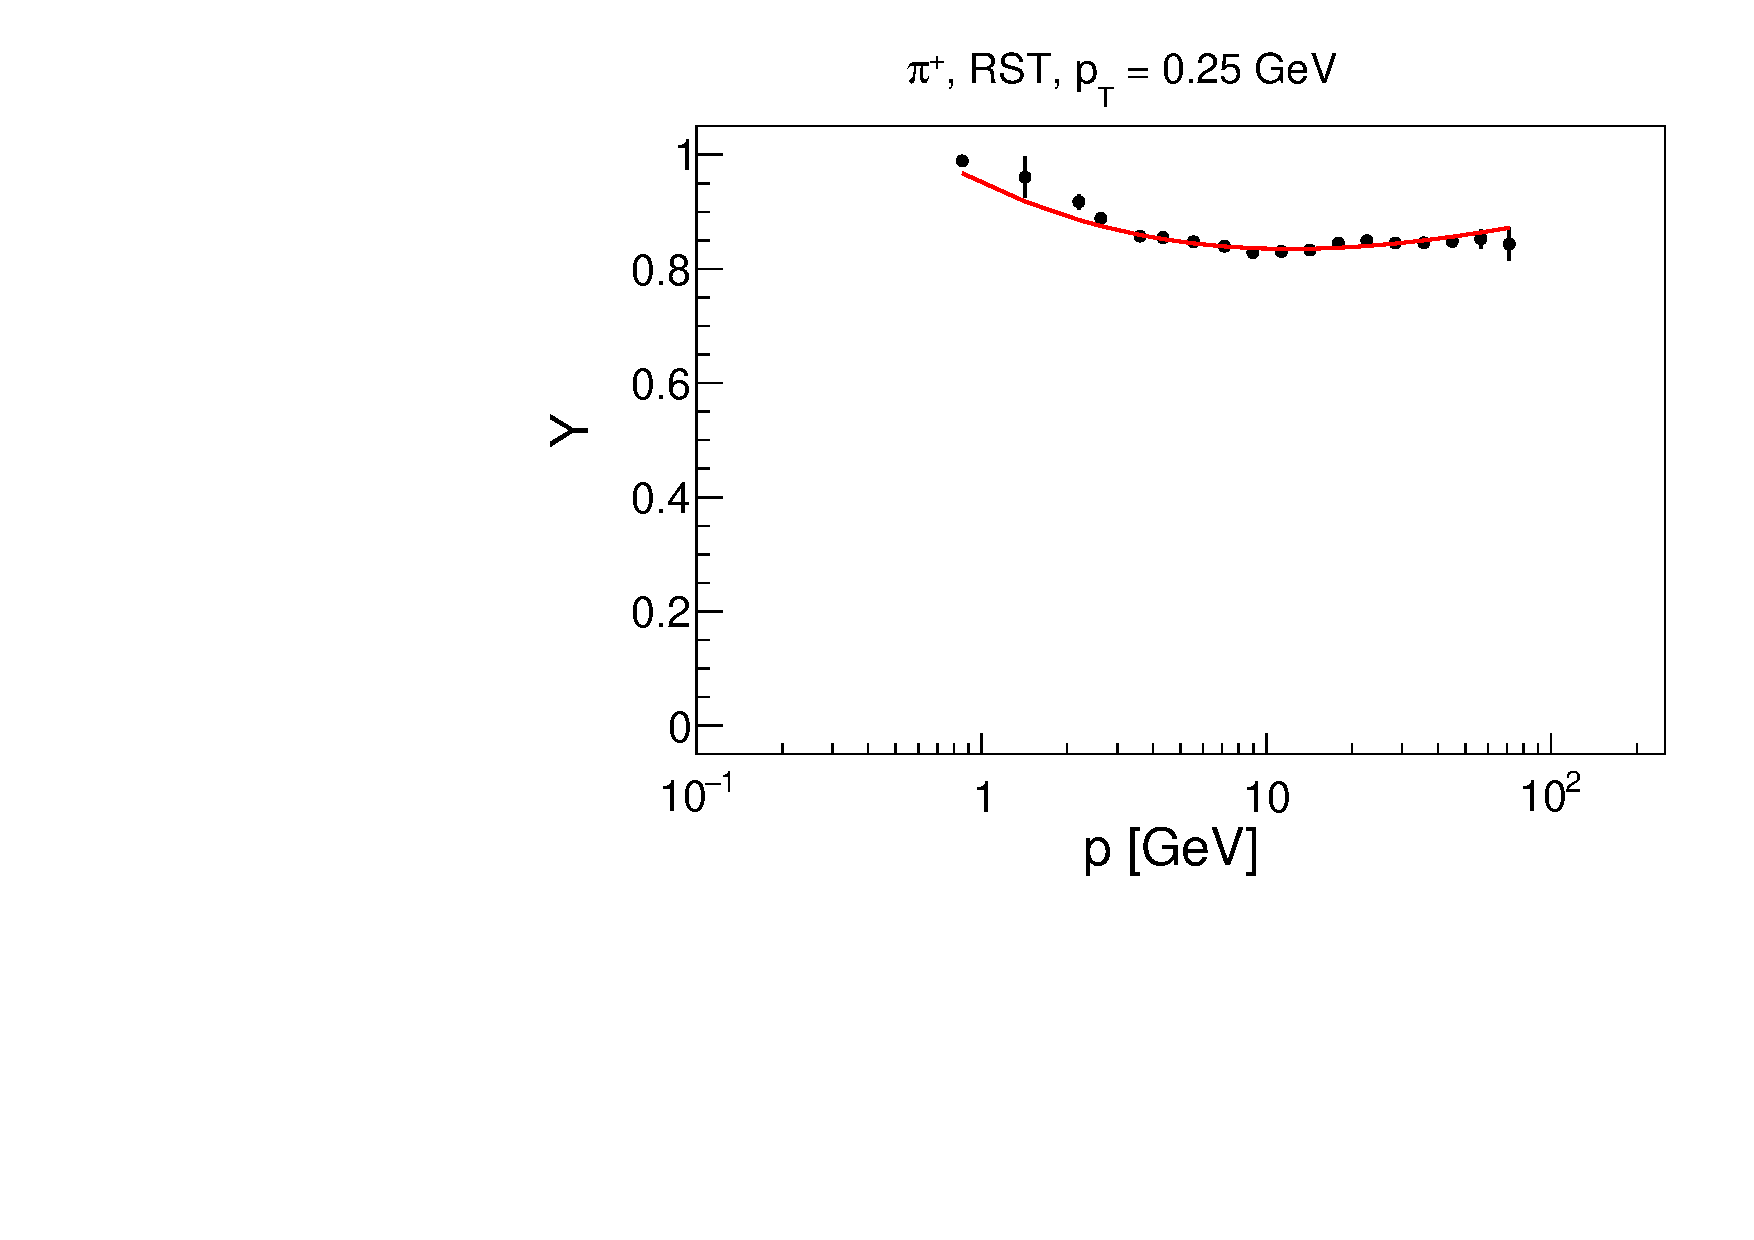
\includegraphics[clip, rviewport=0 0 1 1,width=0.4\textwidth]{dedx/fake_yield_example_158}
  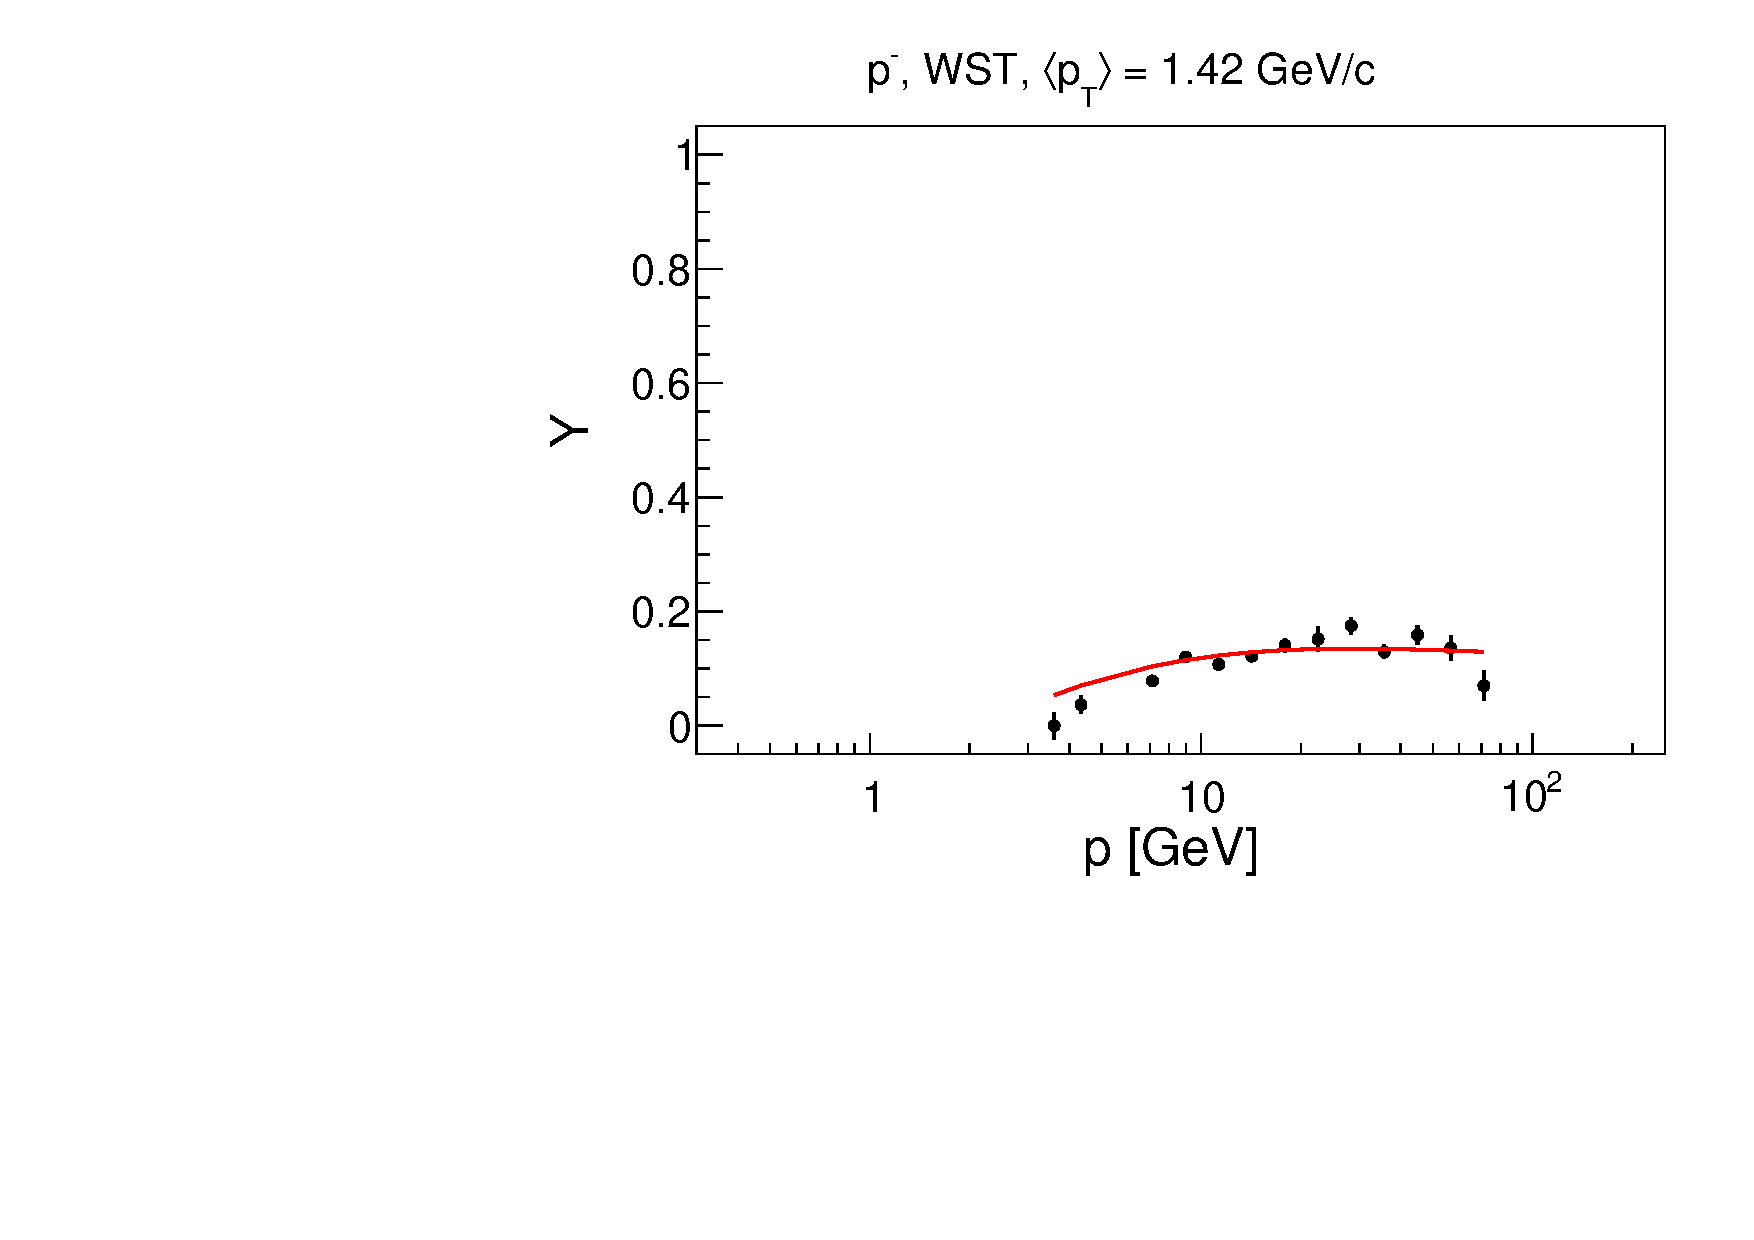
\includegraphics[clip, rviewport=0 0 1 1,width=0.4\textwidth]{dedx/fake_yield_example_two_158}

  \vspace{0.5cm}
  
  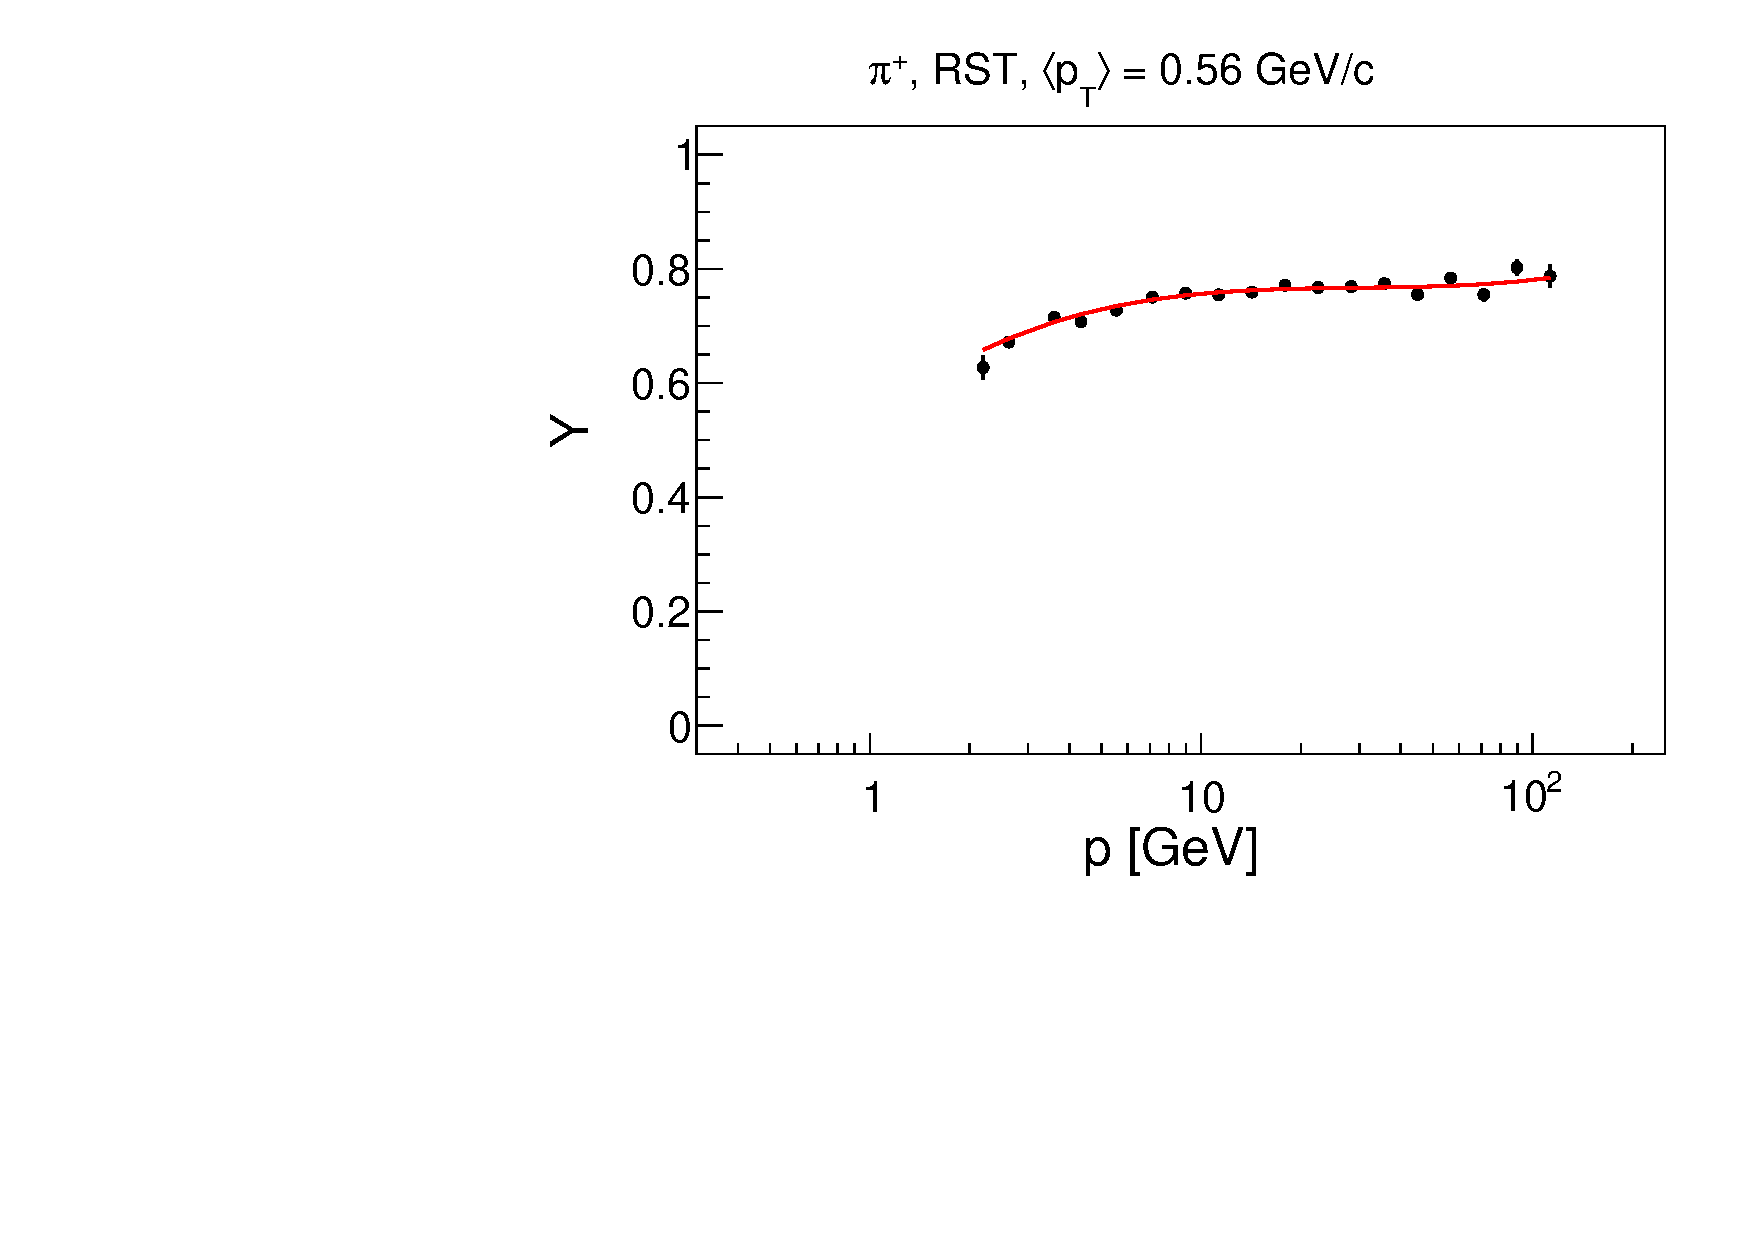
\includegraphics[clip, rviewport=0 0 1 1,width=0.4\textwidth]{dedx/fake_yield_example_350}
  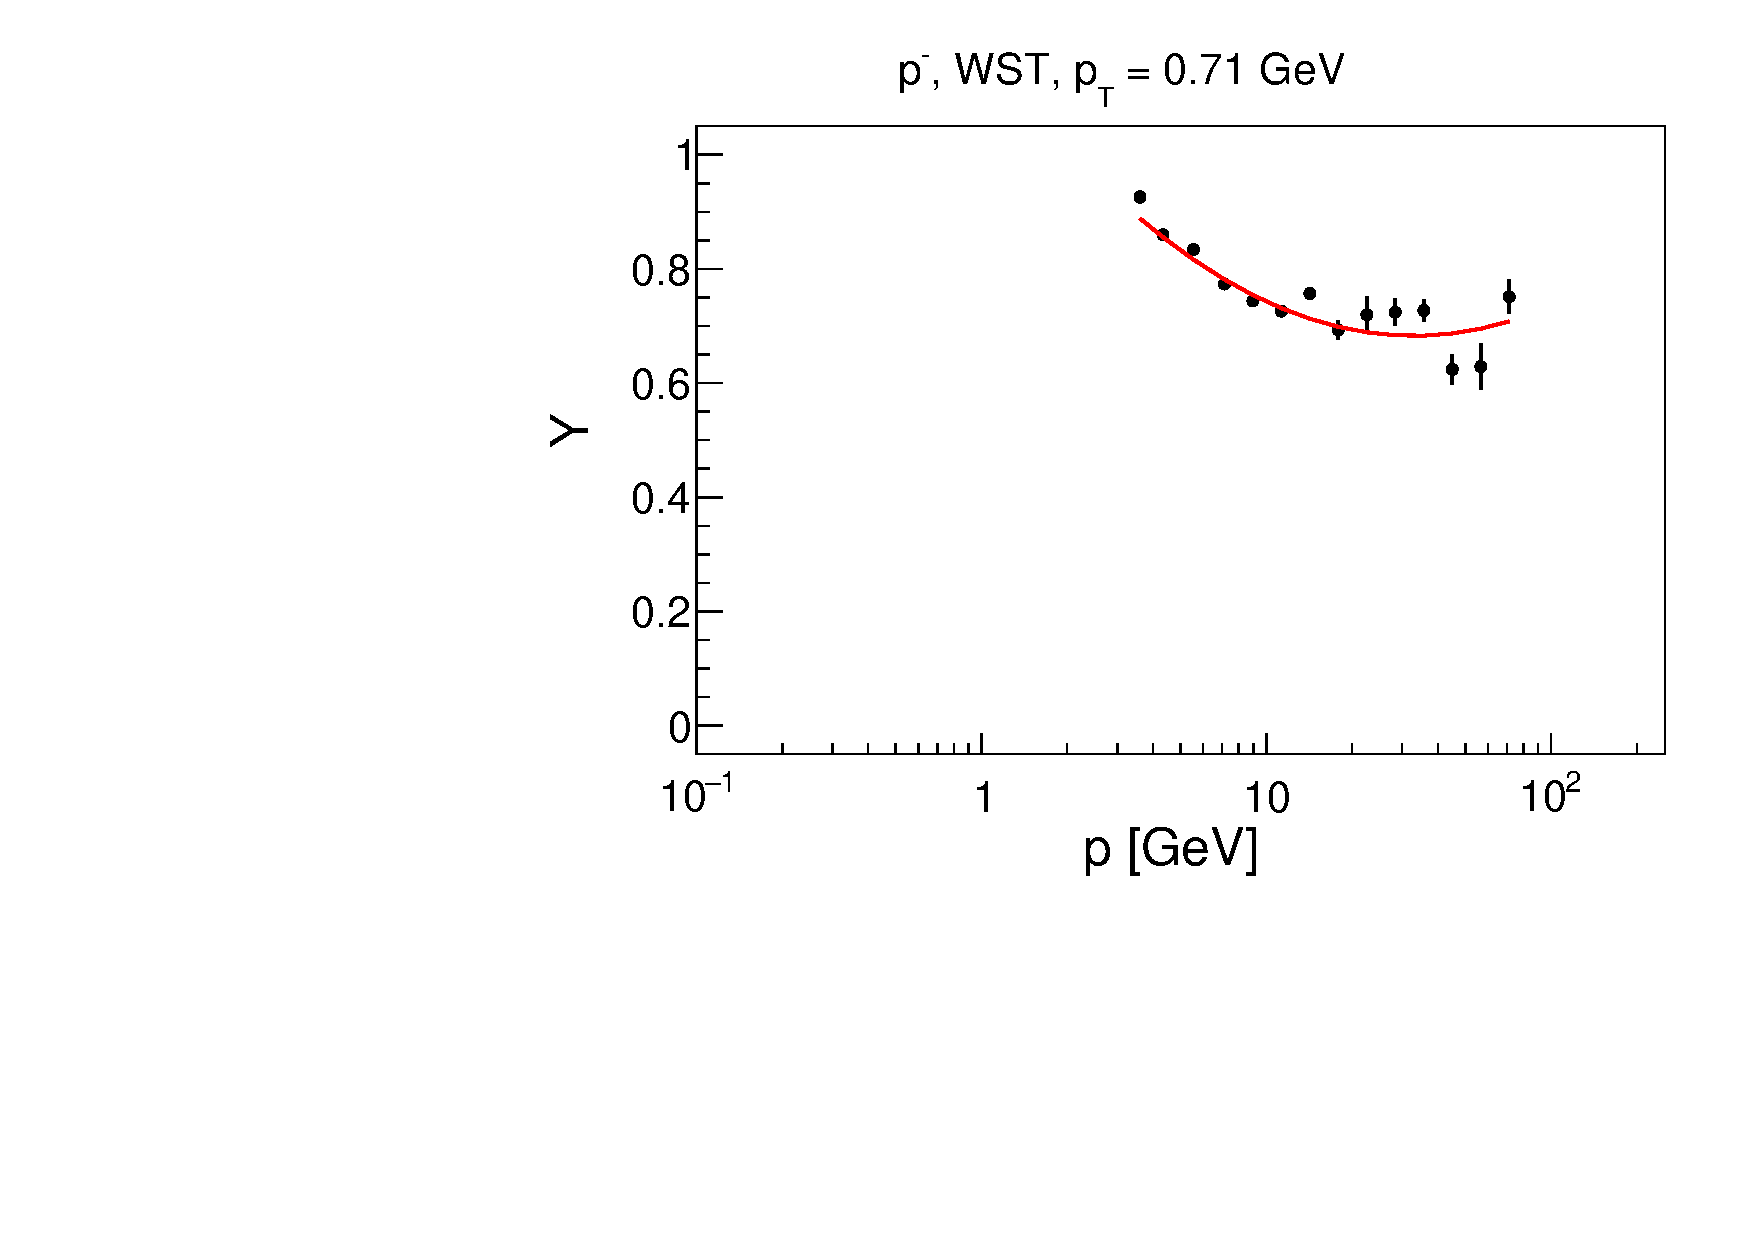
\includegraphics[clip, rviewport=0 0 1 1,width=0.4\textwidth]{dedx/fake_yield_example_two_350}

  \caption{Examples of the parametrization of the particle fractions to be used to create the Simulated Data Ensembles. The plots on the top and on the bottom are for the 158 and 350 \GeVc dataset, respectively.}
  \label{fig:hadron:dedx:fit:fakeyield}
\end{figure}


After sampling a particle type, the \dedx associated to each
track is sampled by following the \dedx model.
The model parameters are set as the ones obtained by the \dedx fit
of the data that are shown in~\cref{sec:hadron:dedx:fitresults}.
A set of $\approx 1000$ simulated sets, for each beam energy,
were created by following the description above and
fitted afterwards. As the result, we obtain the distributions
of the fitted fractions for each particle and phase space bin.

First we can evaluate the relative standard deviation,
defined as $\sigma_r = \sigma_Y/\langle Y\rangle$, where
$\sigma_Y$ is the standard deviation of the fraction $Y$
and $\langle Y \rangle$ is its average value.
In~\cref{fig:hadron:dedx:fit:fake:relsig158r} we show
one example of $\sigma_r$ for the RST and 158 \GeVc case.
The remaining cases are shown
in~\cref{fig:hadron:dedx:fit:fake:relsig158w,fig:hadron:dedx:fit:fake:relsig350r,fig:hadron:dedx:fit:fake:relsig350w}. Only \pions, \kaons and \protons are shown
because these are the particles of interested of this analysis.
Second, we can evaluate the relative bias, defined as
$\delta_r = \langle \Delta Y/ Y \rangle$, where $\Delta Y$
is the difference between the fitted and the true fraction,
being the true fraction computed while the particle types
of each track are sampled.
In~\cref{fig:hadron:dedx:fit:fake:reldev158r} we show examples
of $\delta_r$ for RST and 158 \GeVc case, while the remaning
cases are shown
in~\cref{fig:hadron:dedx:fit:fake:reldev158w,fig:hadron:dedx:fit:fake:reldev350r,fig:hadron:dedx:fit:fake:reldev350w}.

%%%%%%%%%% FAKE REL SIG %%%%%%%%%%%%%%
\begin{figure}[!ht]
  \centering
  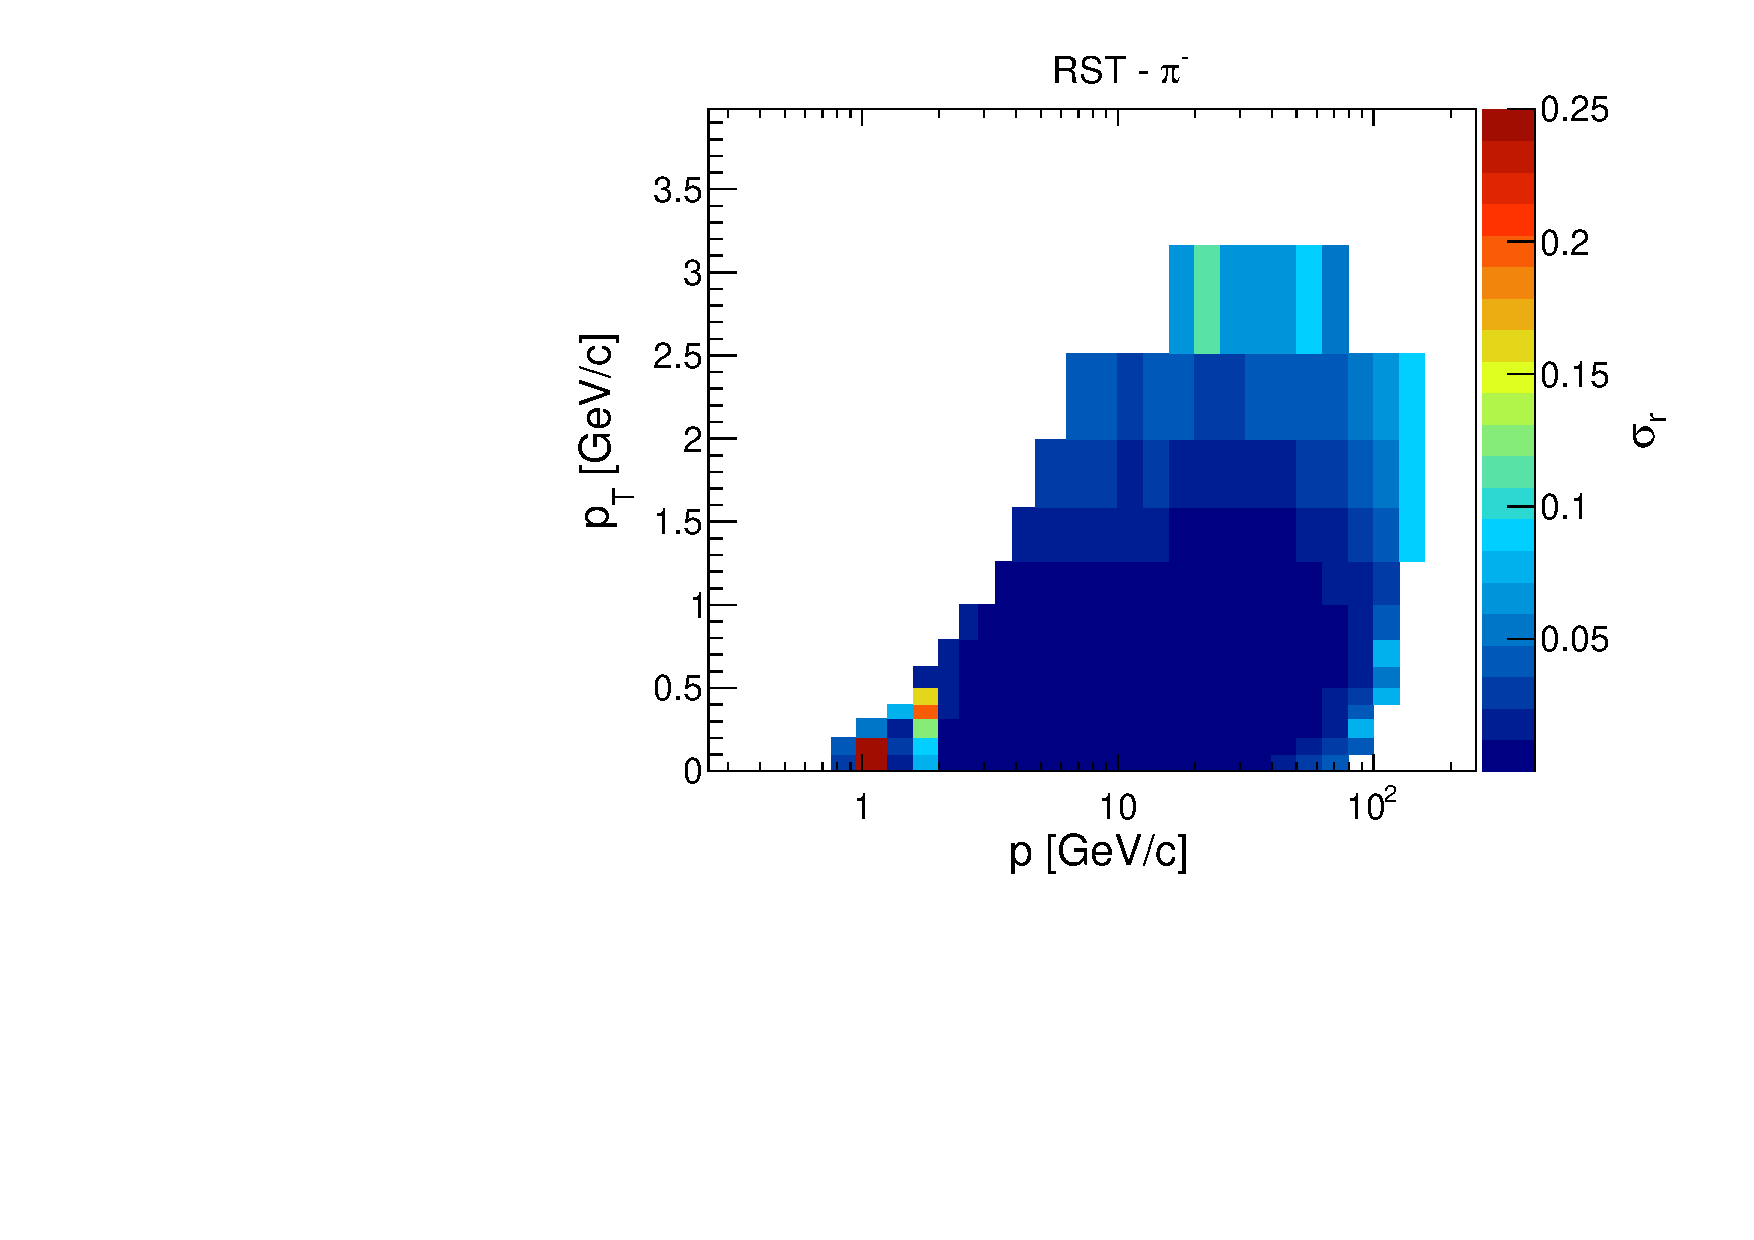
\includegraphics[clip, rviewport=0 0.13 1 0.94,width=0.4\textwidth]{dedx/fake_rel_sig_158_fl0_v0_c0_p1}
  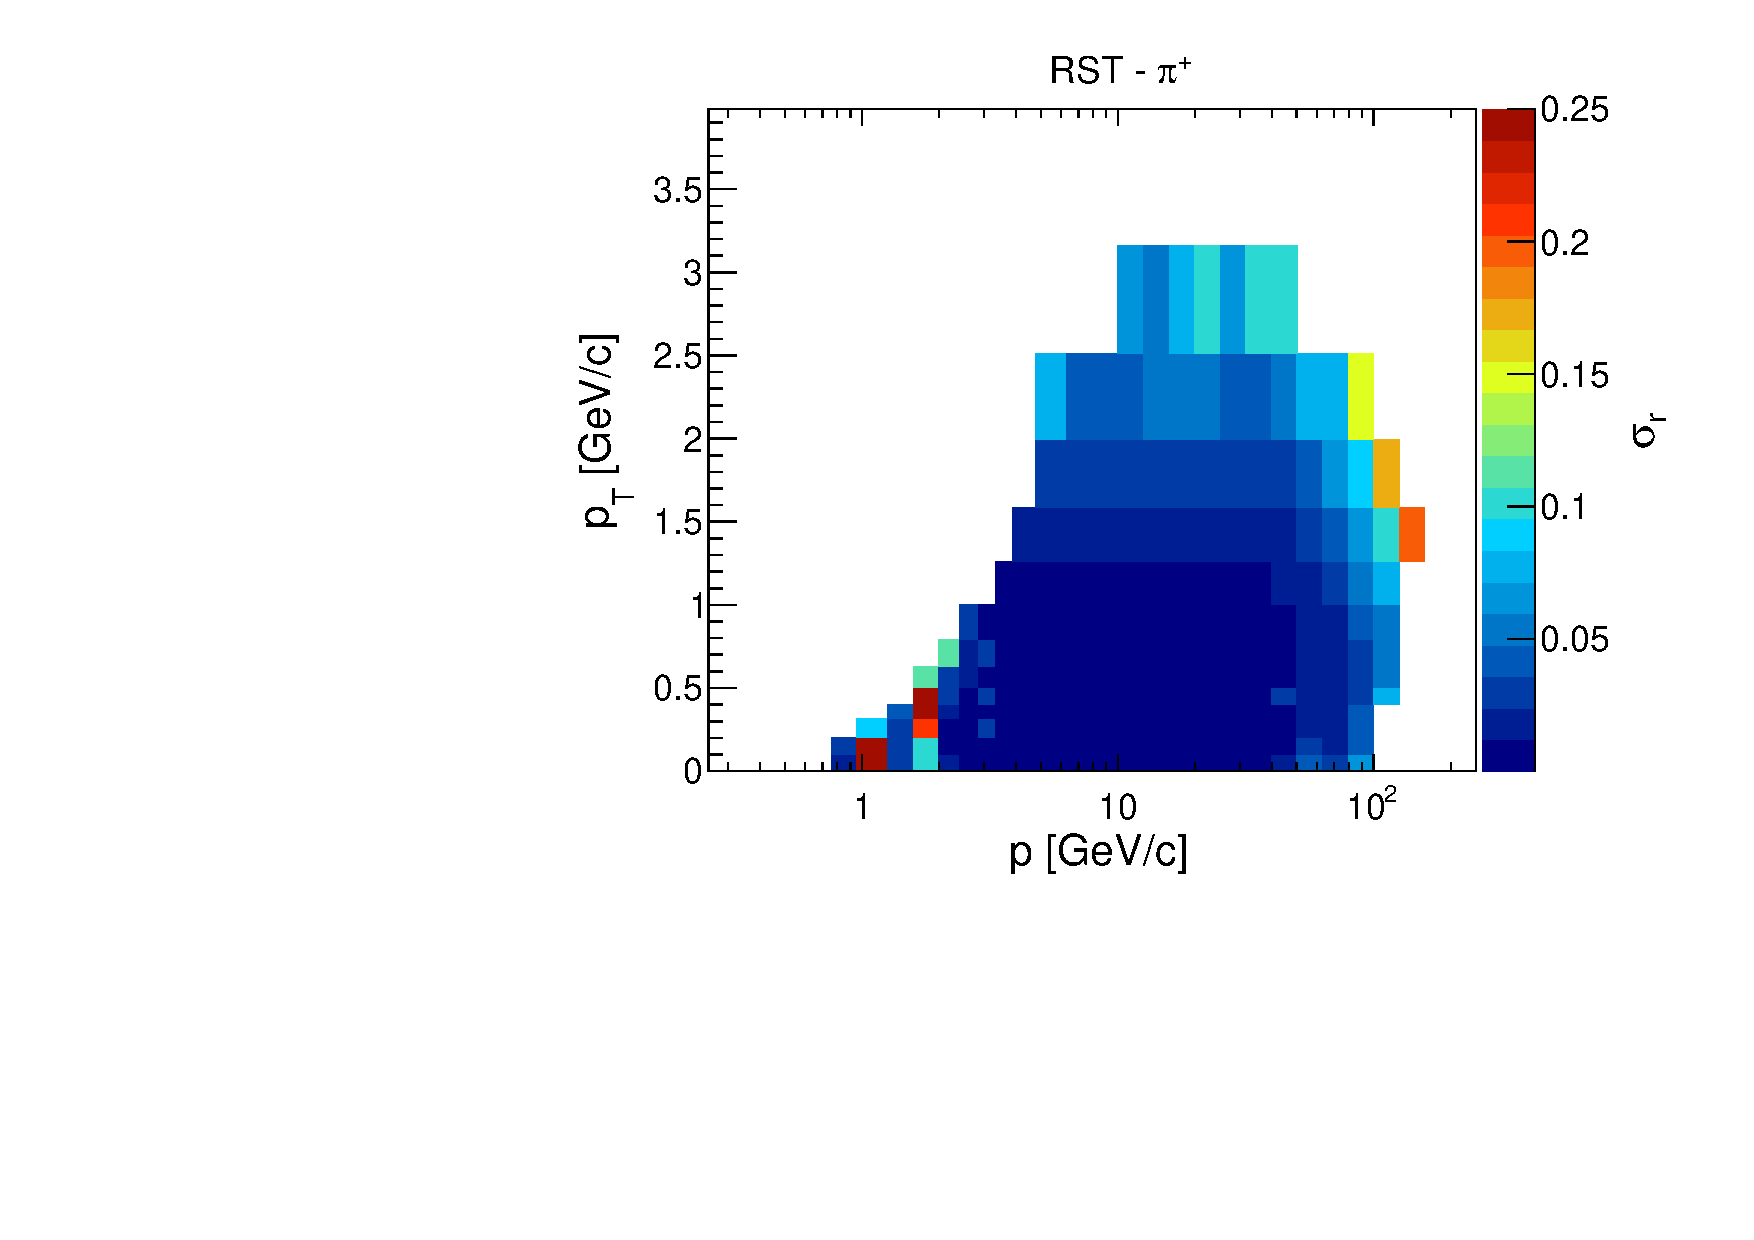
\includegraphics[clip, rviewport=0 0.13 1 0.94,width=0.4\textwidth]{dedx/fake_rel_sig_158_fl0_v0_c1_p1}

  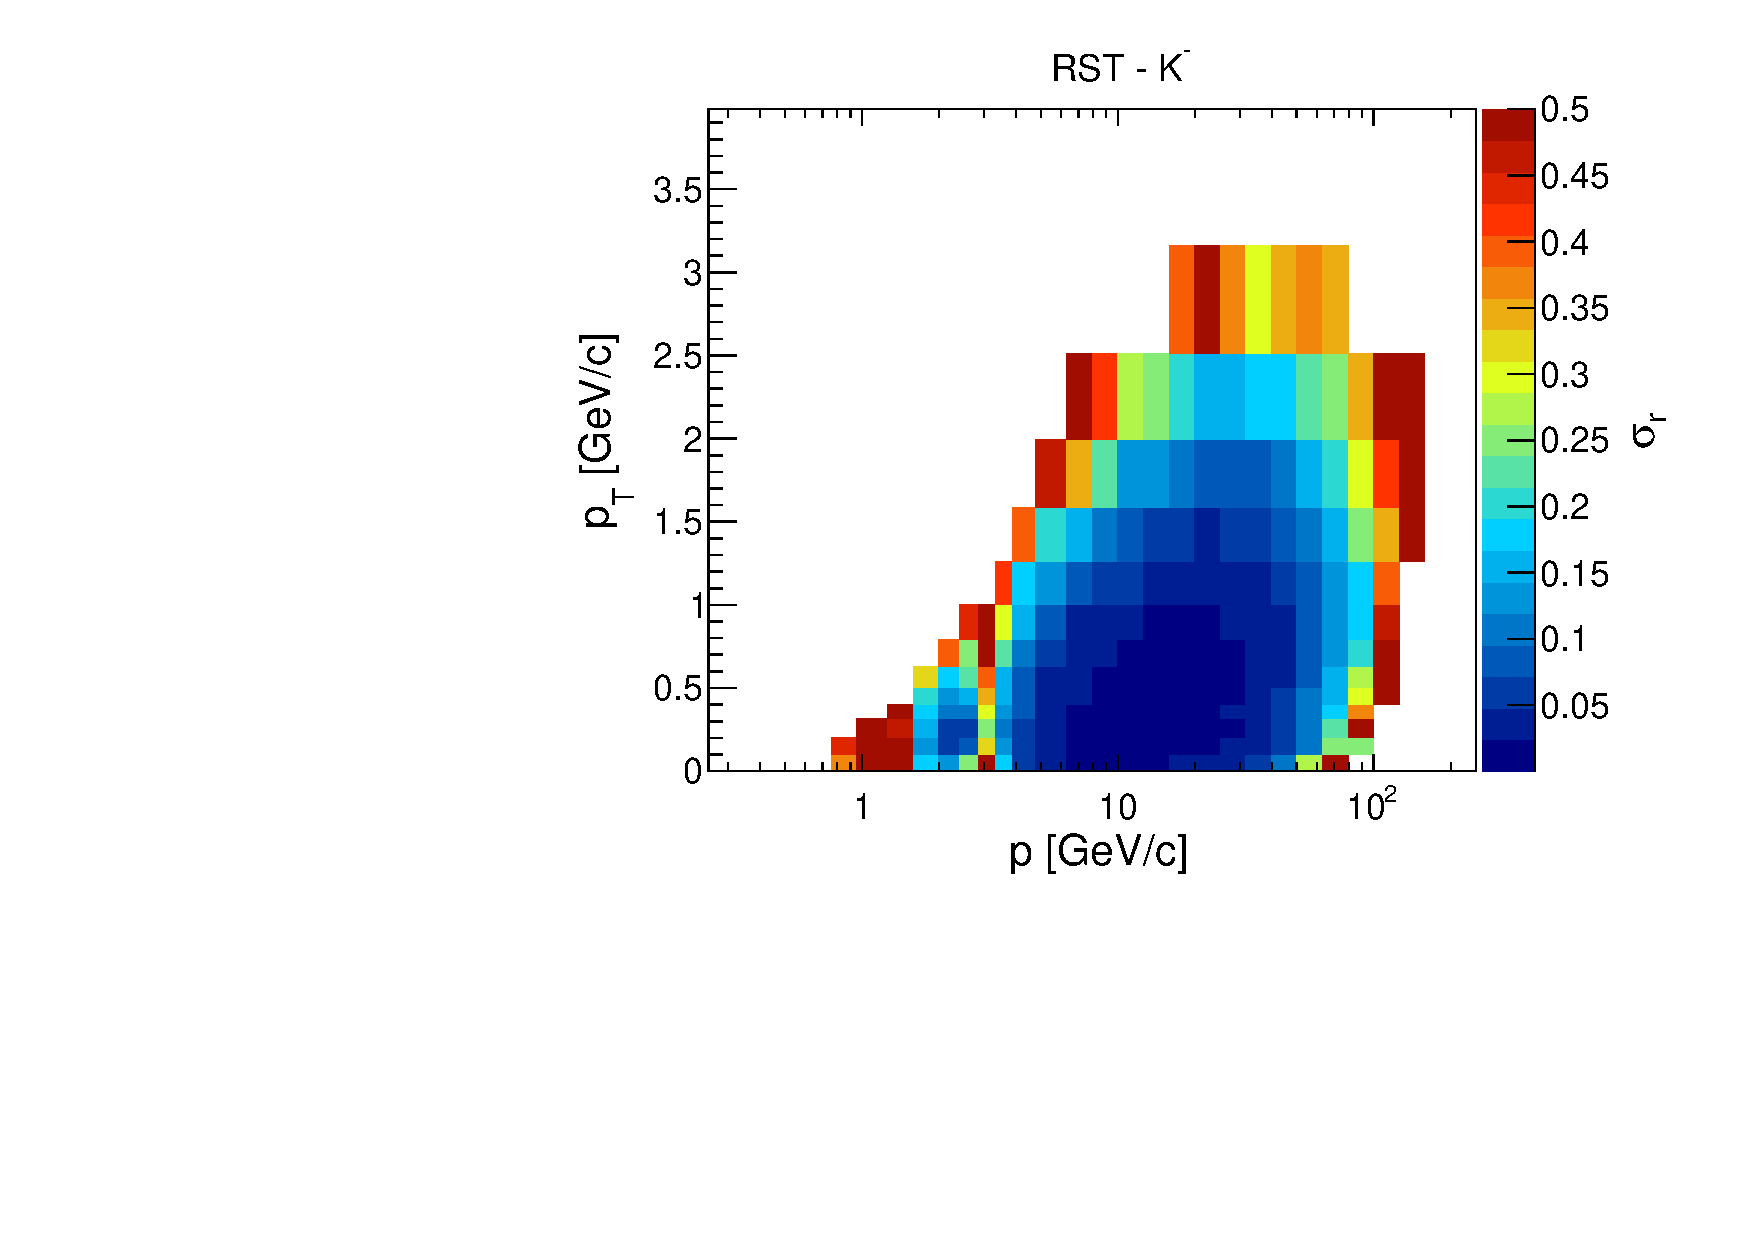
\includegraphics[clip, rviewport=0 0.13 1 0.94,width=0.4\textwidth]{dedx/fake_rel_sig_158_fl0_v0_c0_p2}
  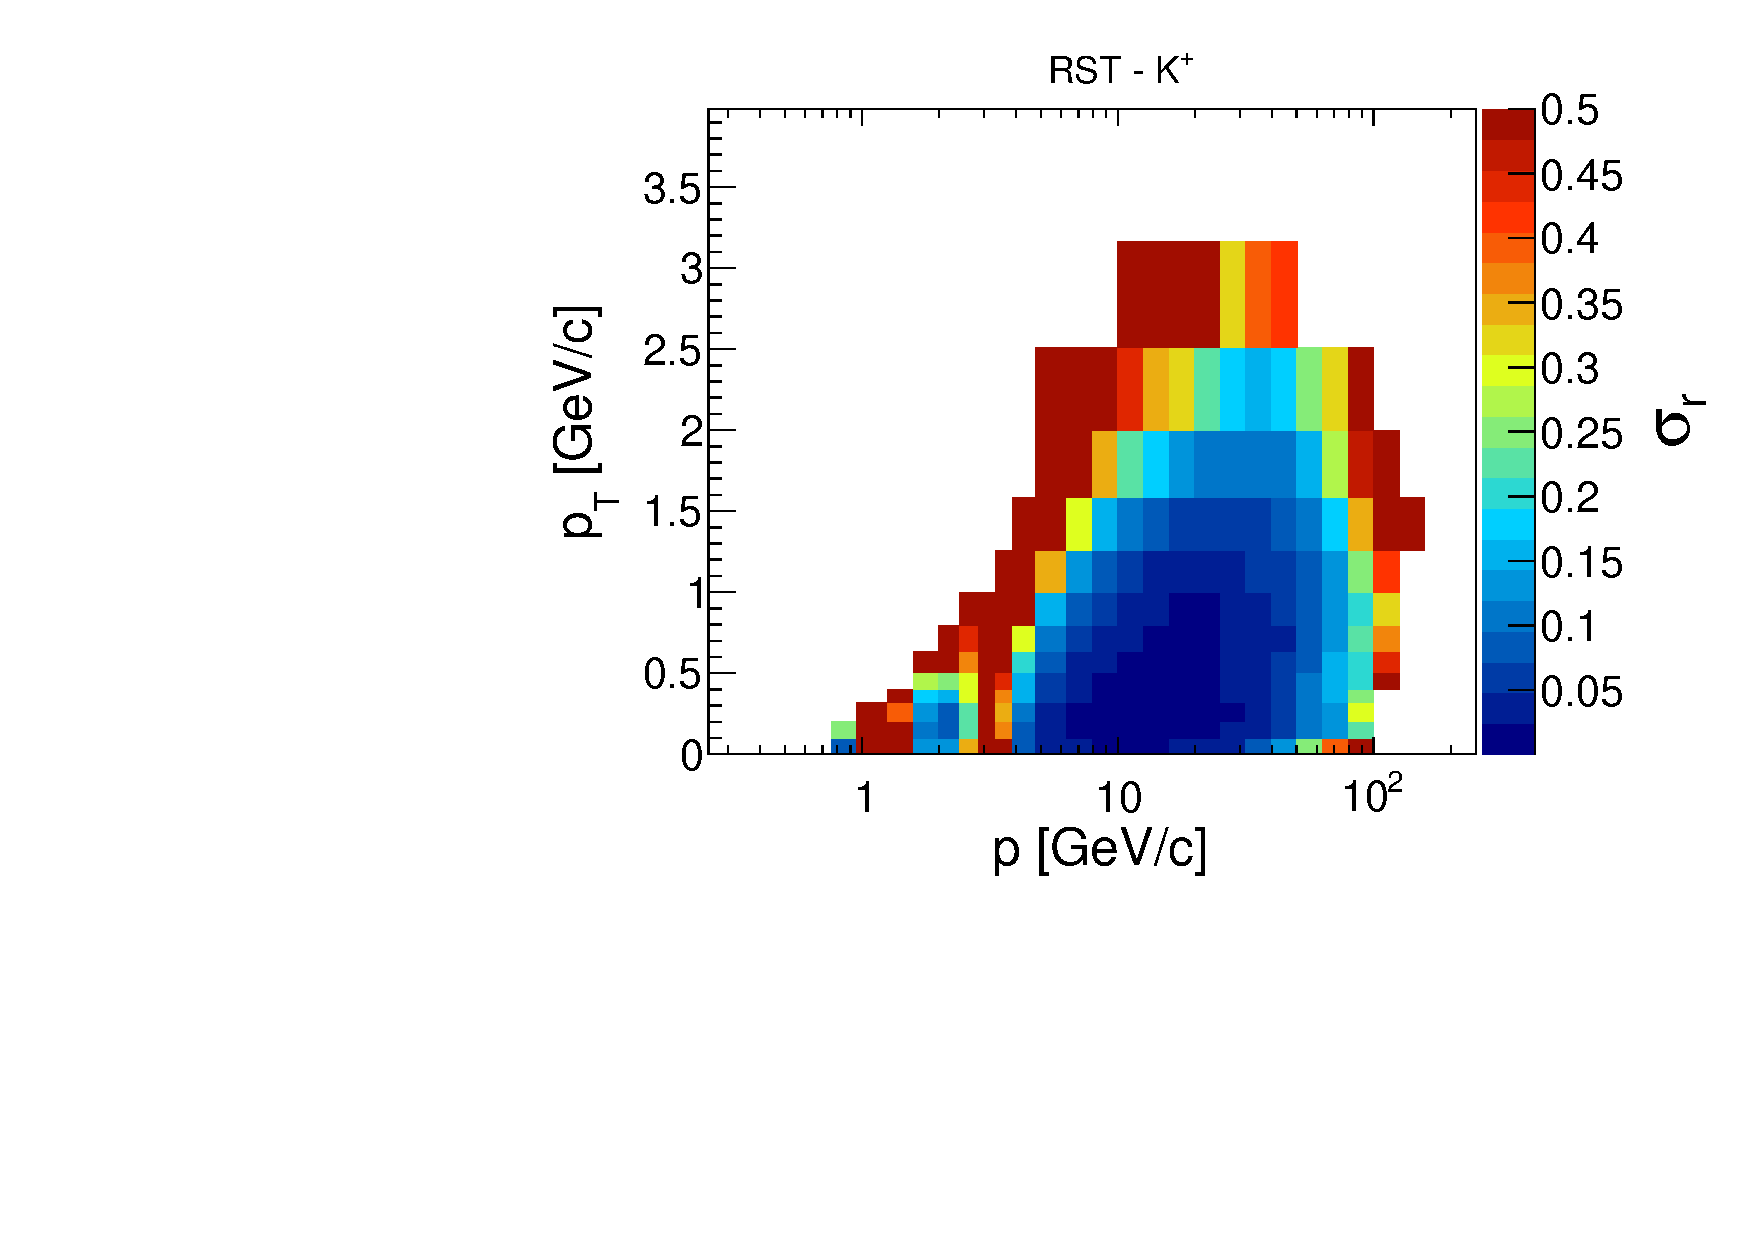
\includegraphics[clip, rviewport=0 0.13 1 0.94,width=0.4\textwidth]{dedx/fake_rel_sig_158_fl0_v0_c1_p2}

  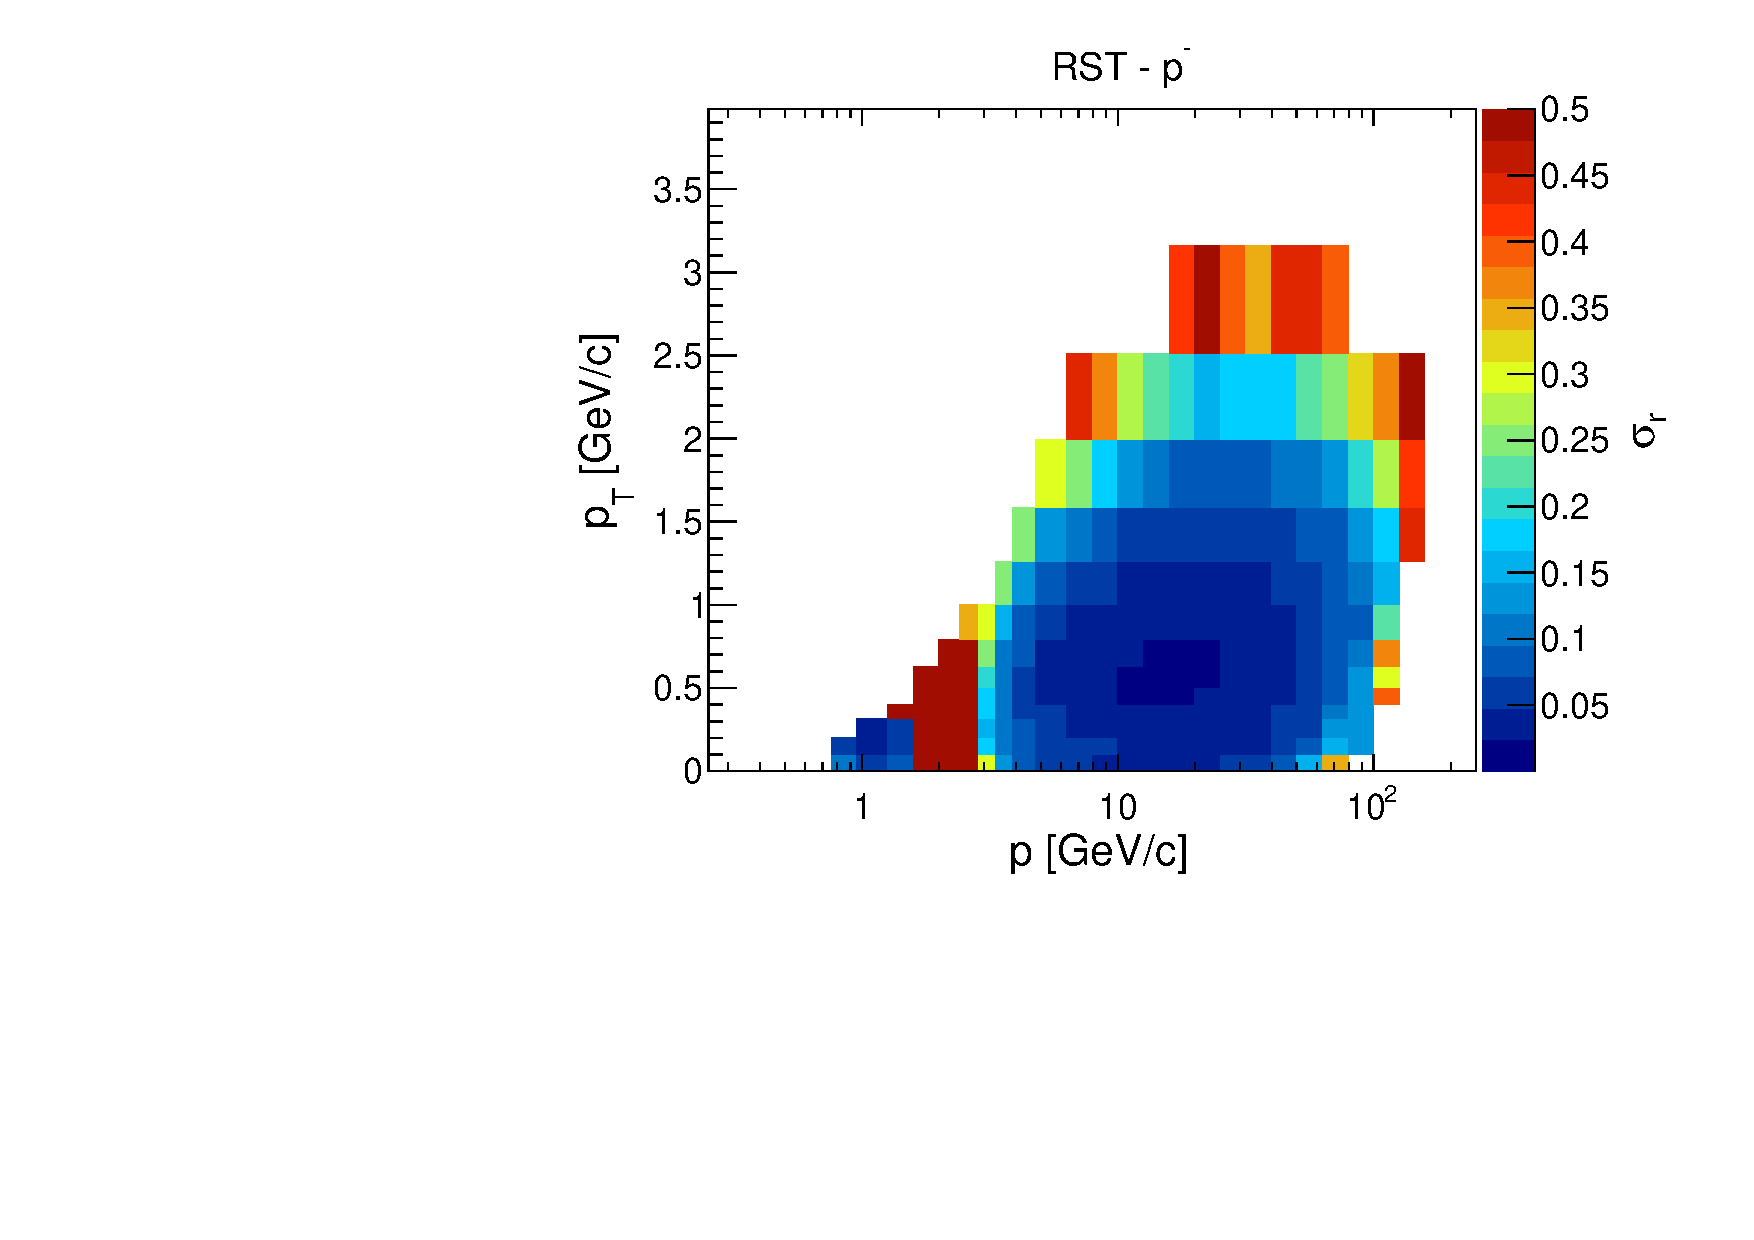
\includegraphics[clip, rviewport=0 0 1 0.94,width=0.4\textwidth]{dedx/fake_rel_sig_158_fl0_v0_c0_p3}
  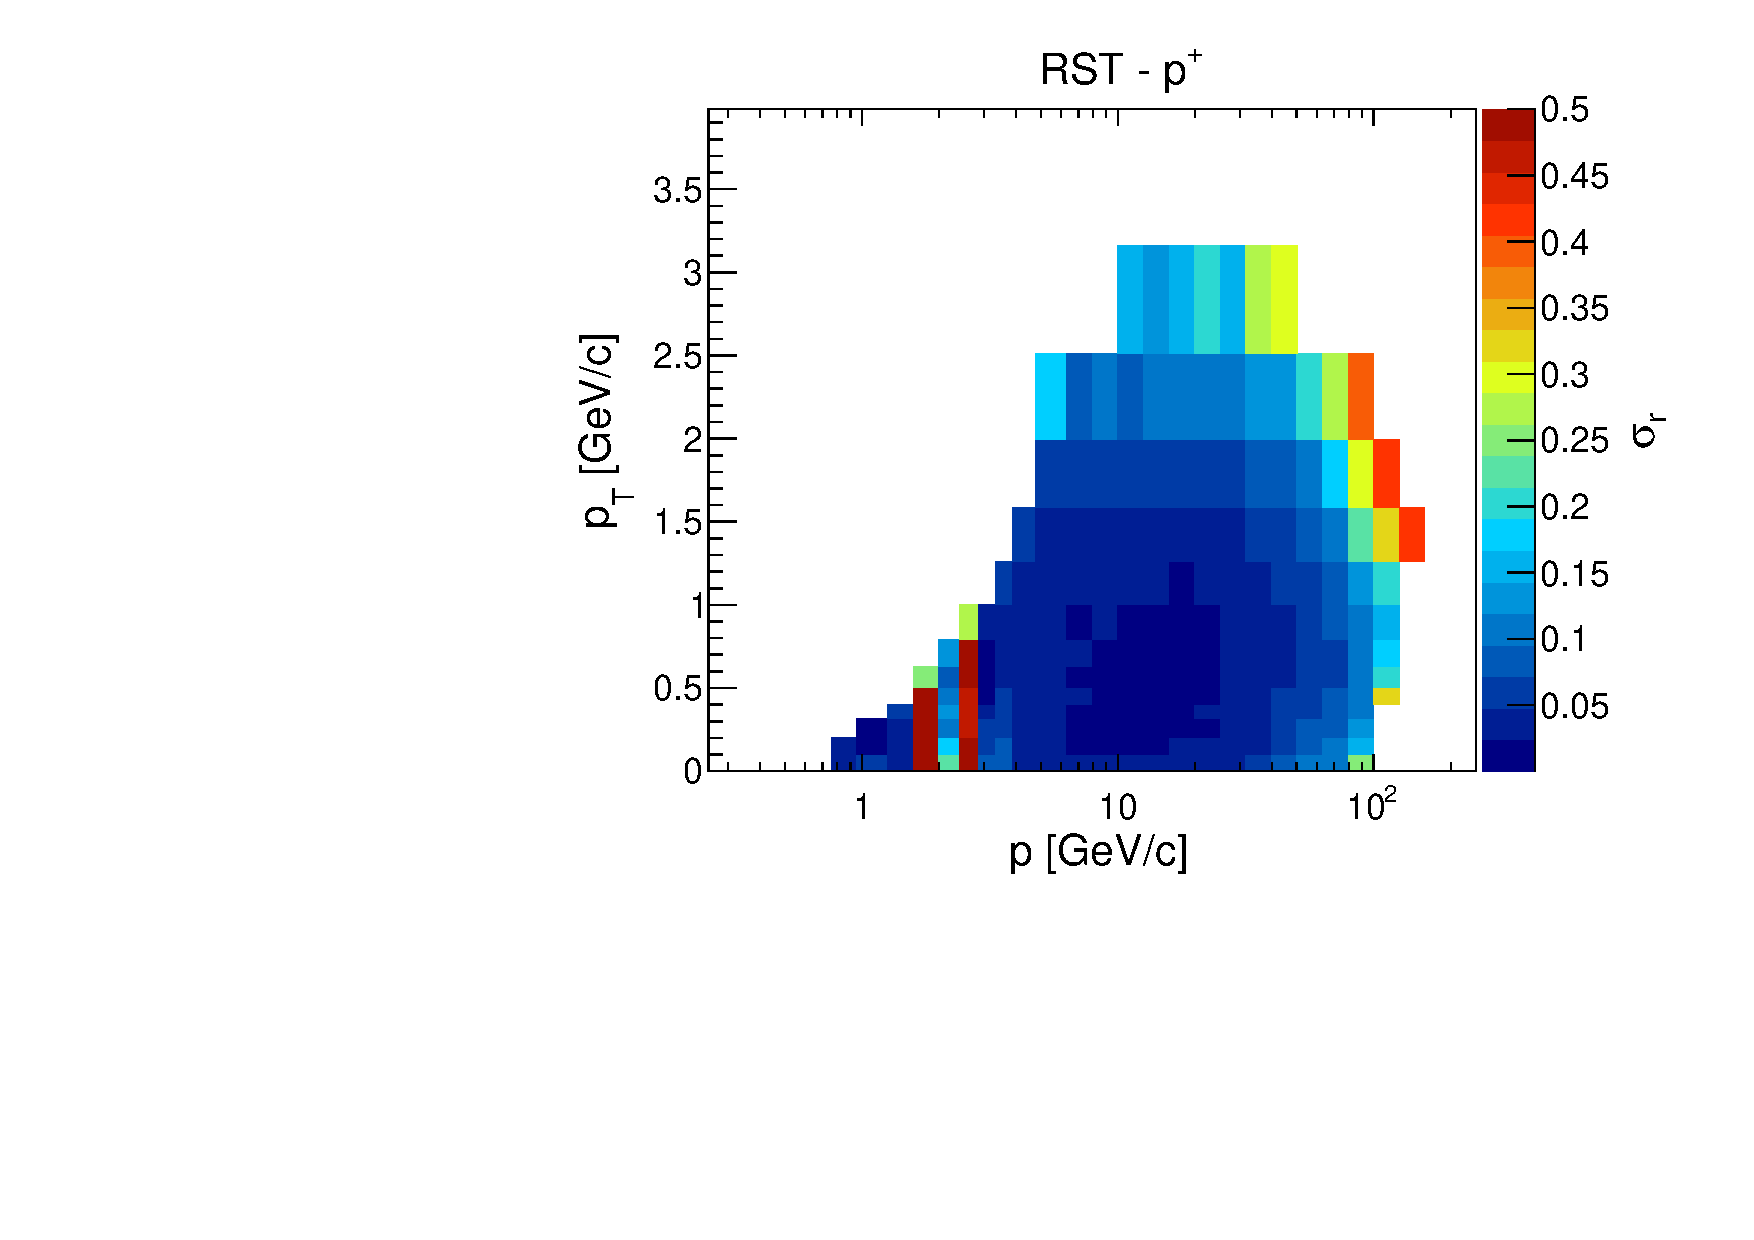
\includegraphics[clip, rviewport=0 0 1 0.94,width=0.4\textwidth]{dedx/fake_rel_sig_158_fl0_v0_c1_p3}


  \caption{Relative standard deviation of the particle fractions obtained with SDEs for RST and 158 \GeVc dataset.}
  \label{fig:hadron:dedx:fit:fake:relsig158r}
\end{figure}


%%%%%%%%%% FAKE REL DEV %%%%%%%%%%%%%%
\begin{figure}[!ht]
  \centering
  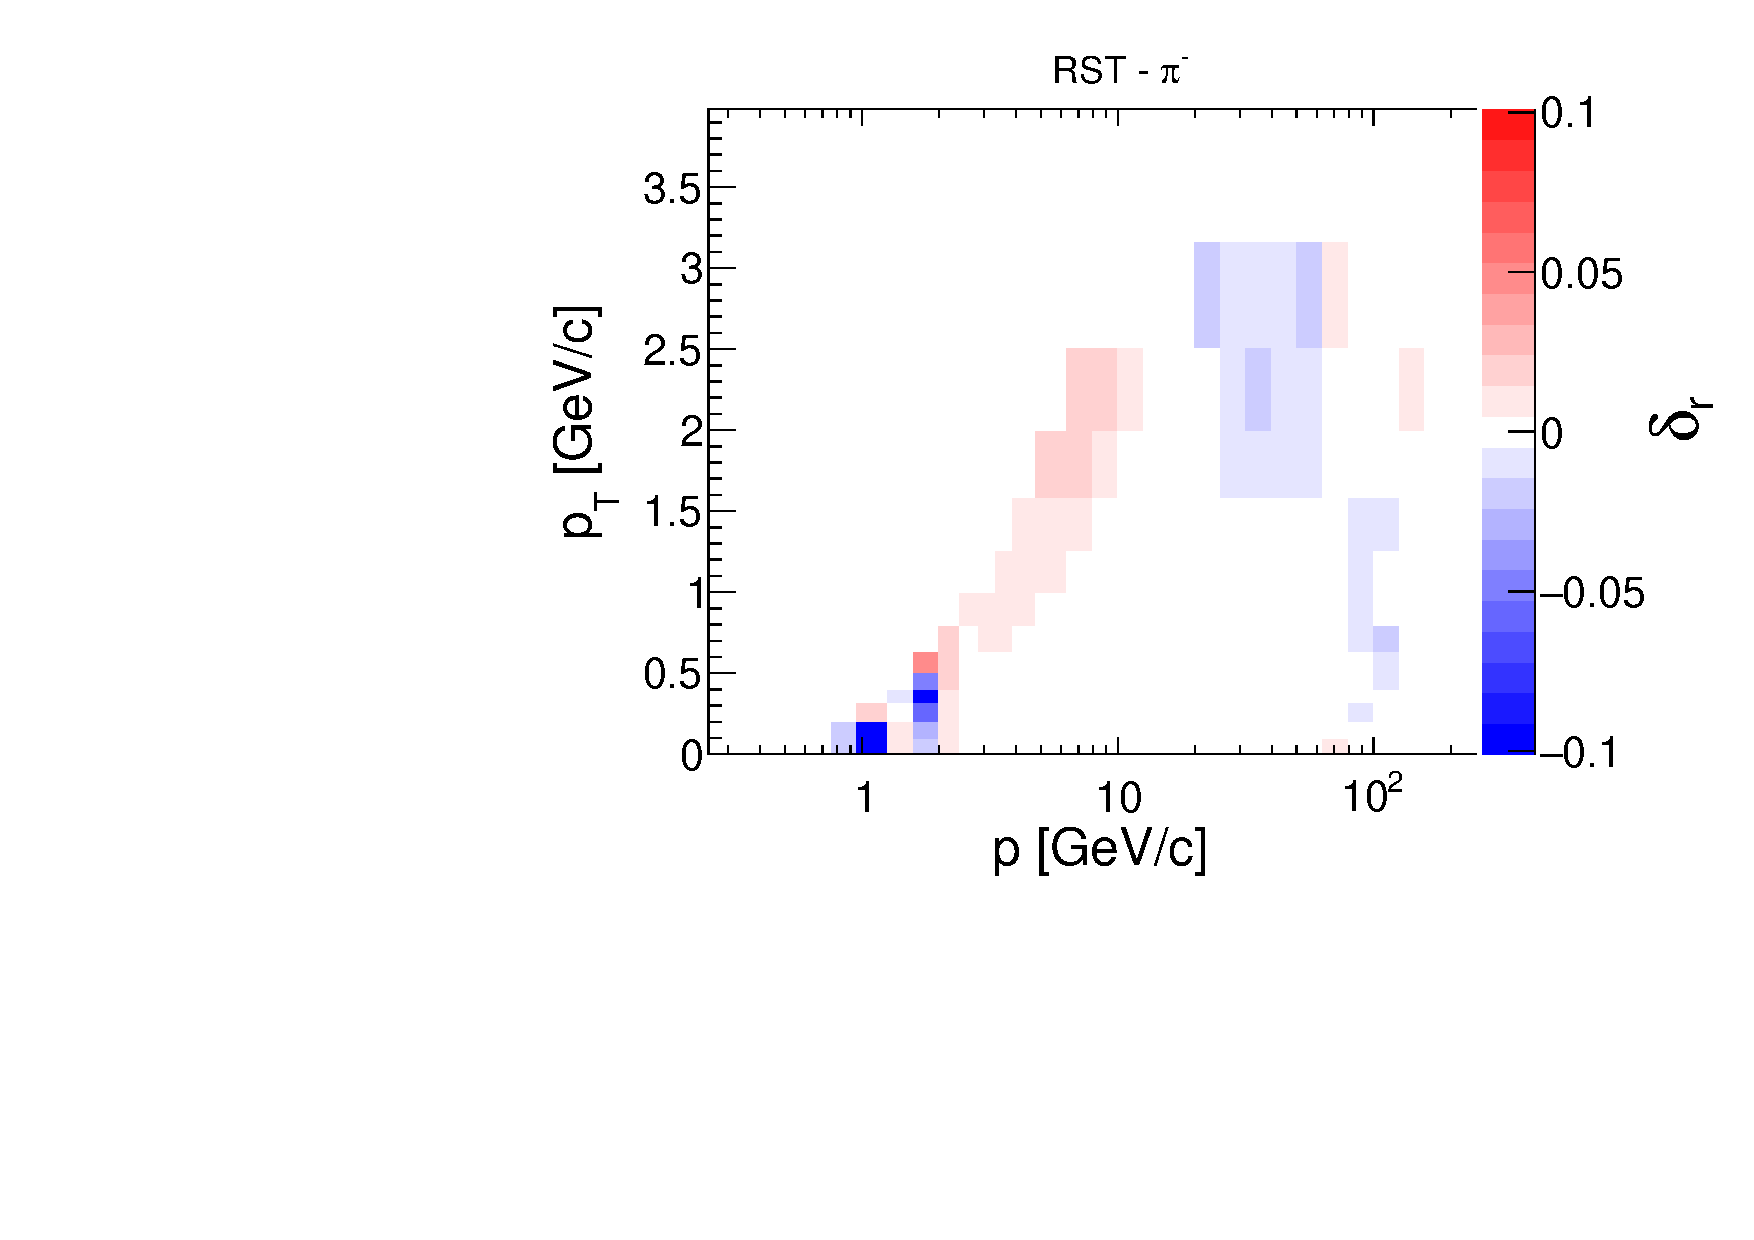
\includegraphics[clip, rviewport=0 0.13 1 0.94,width=0.4\textwidth]{dedx/fake_rel_dev_158_fl0_v0_c0_p1}
  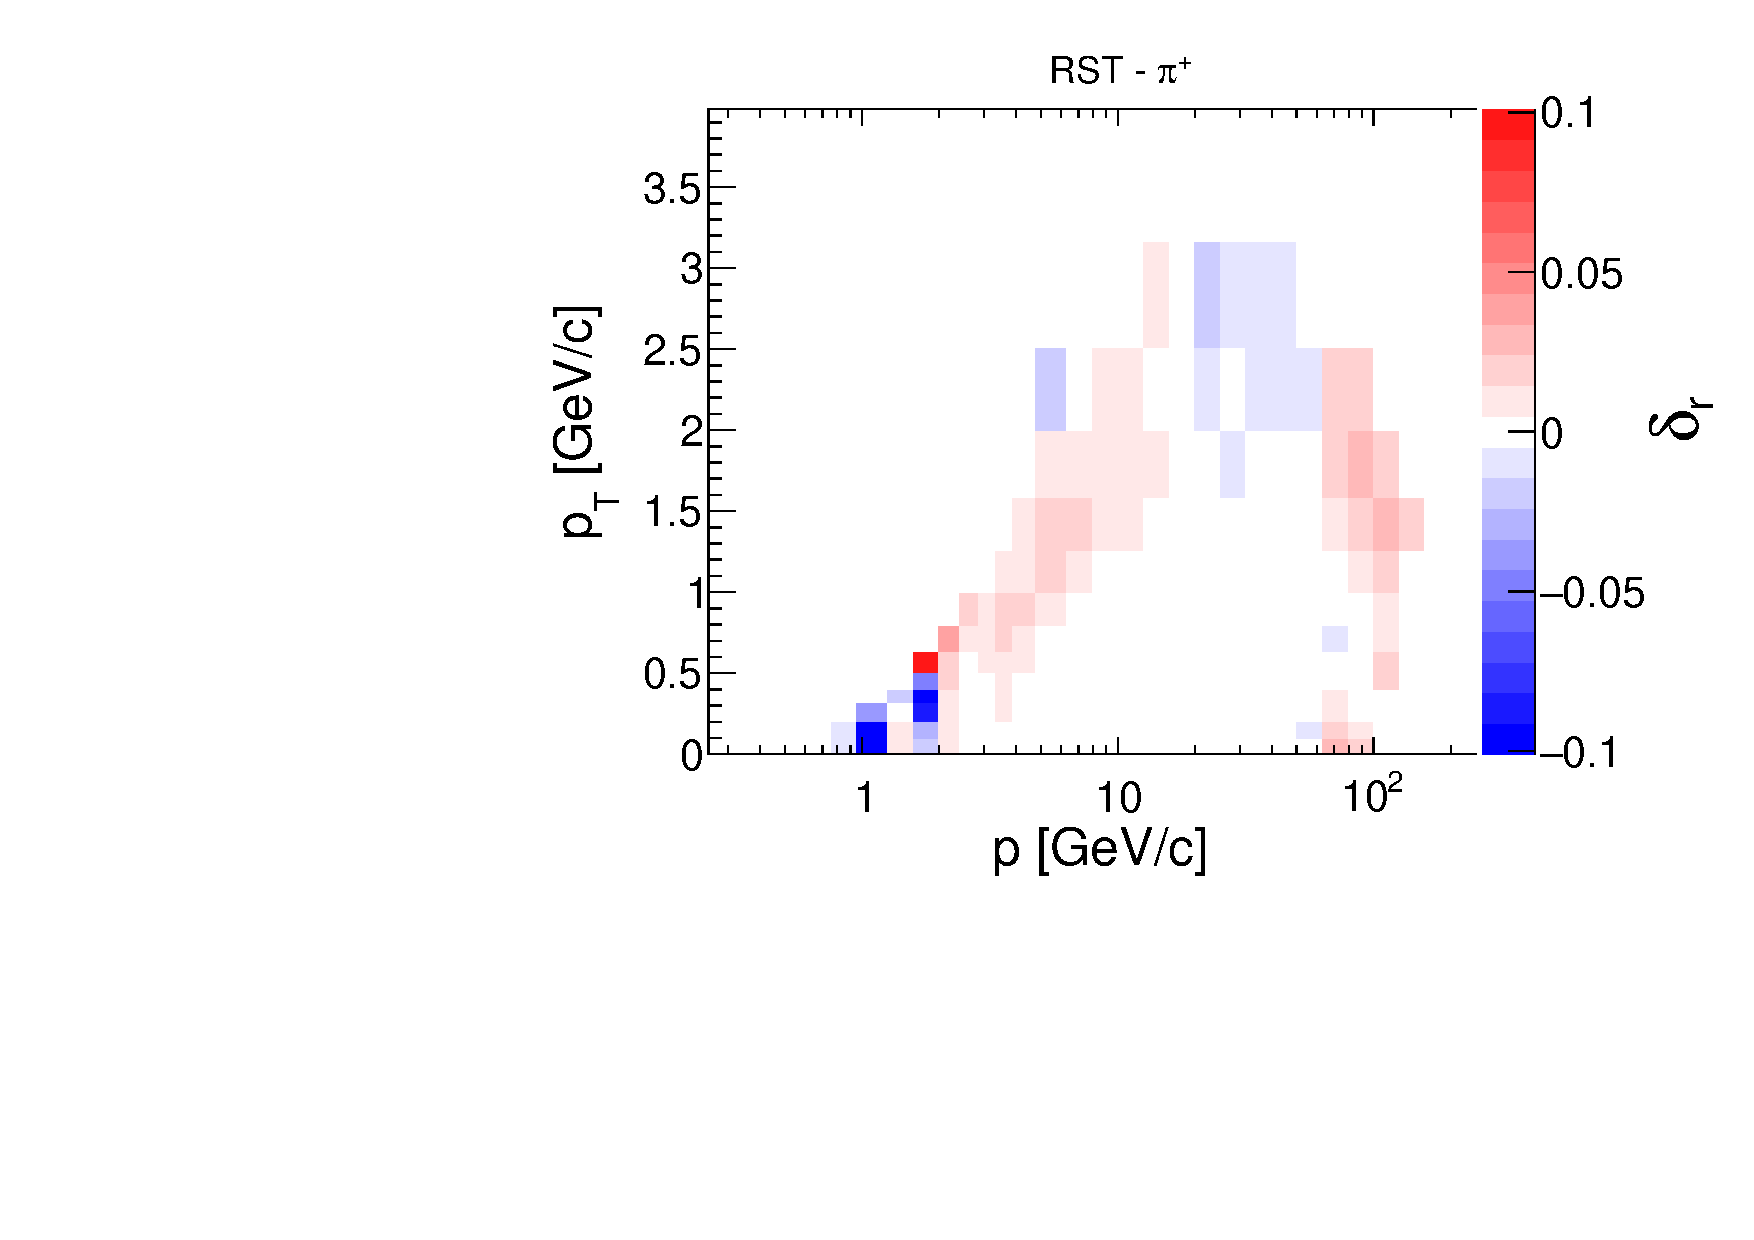
\includegraphics[clip, rviewport=0 0.13 1 0.94,width=0.4\textwidth]{dedx/fake_rel_dev_158_fl0_v0_c1_p1}

  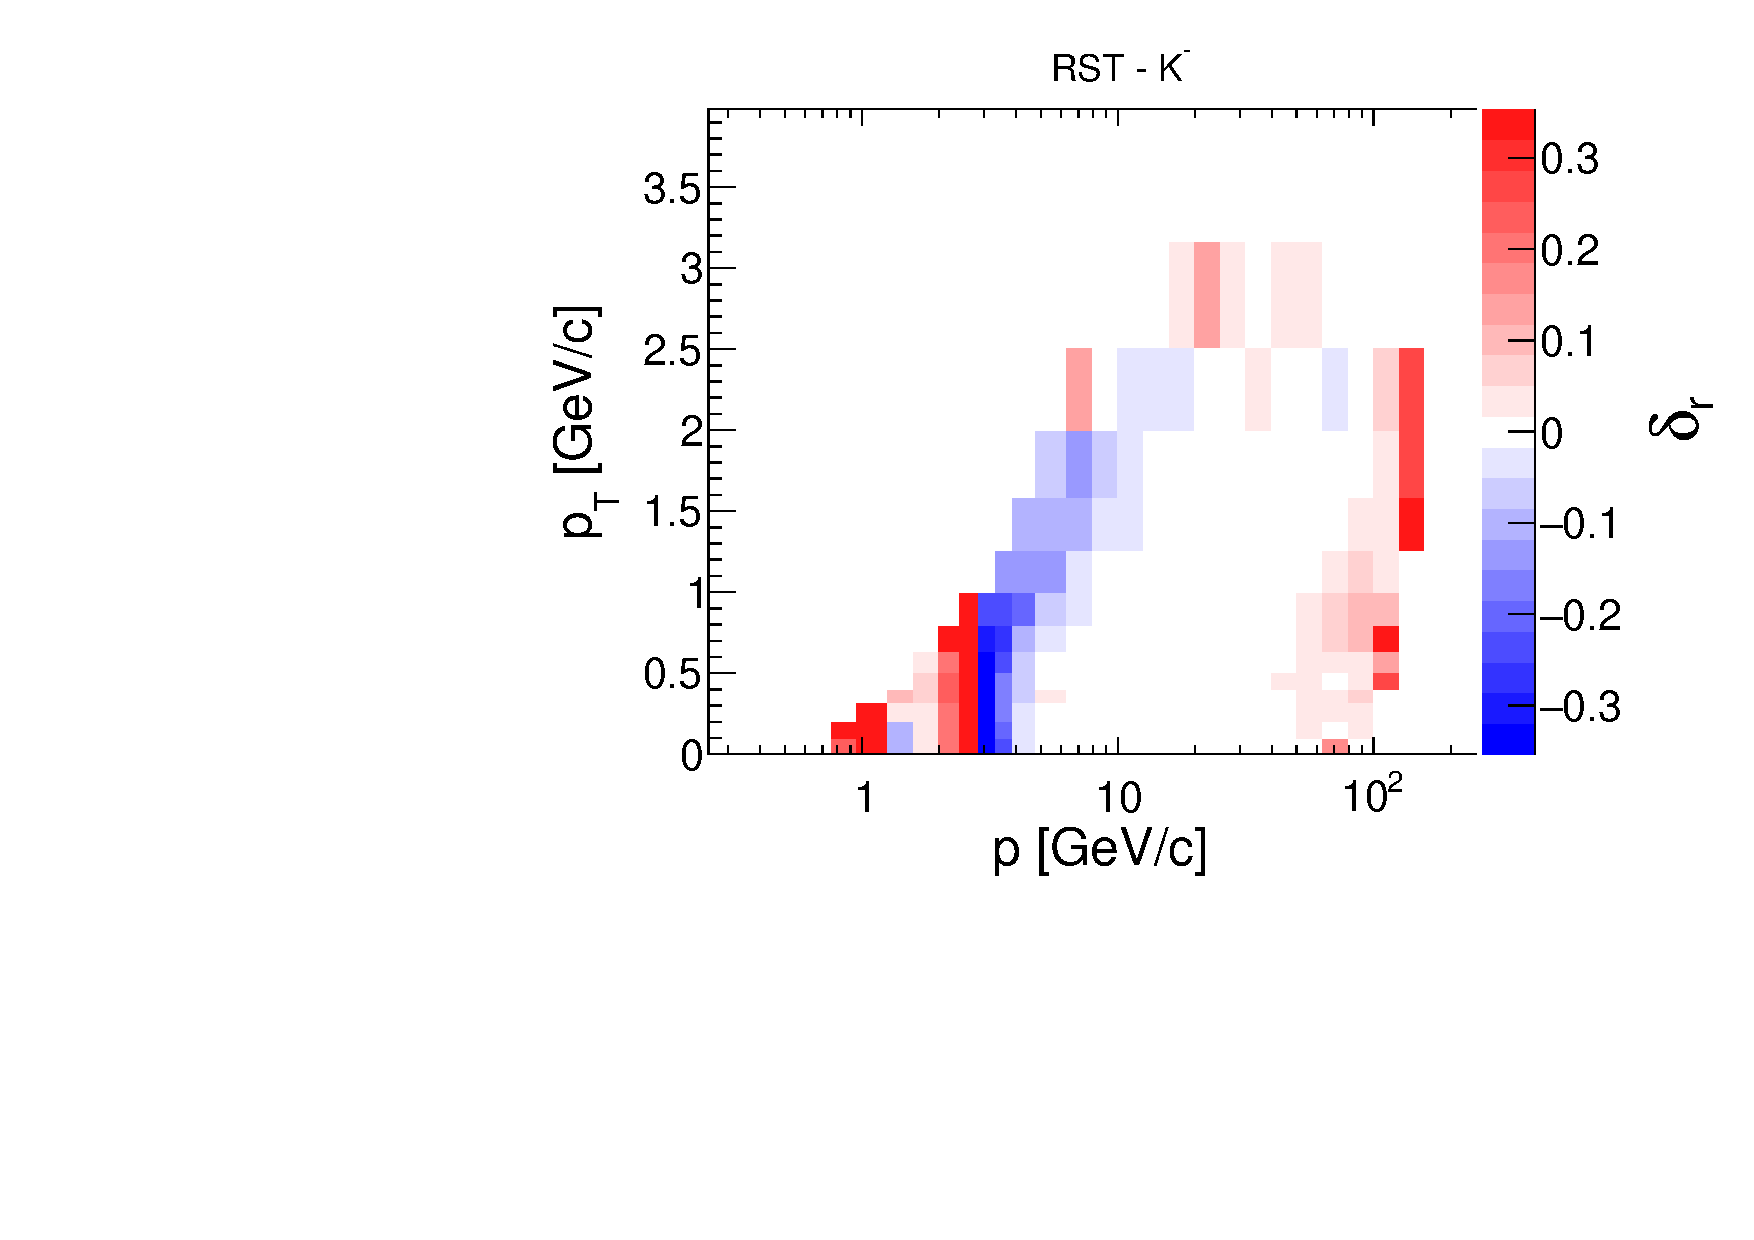
\includegraphics[clip, rviewport=0 0.13 1 0.94,width=0.4\textwidth]{dedx/fake_rel_dev_158_fl0_v0_c0_p2}
  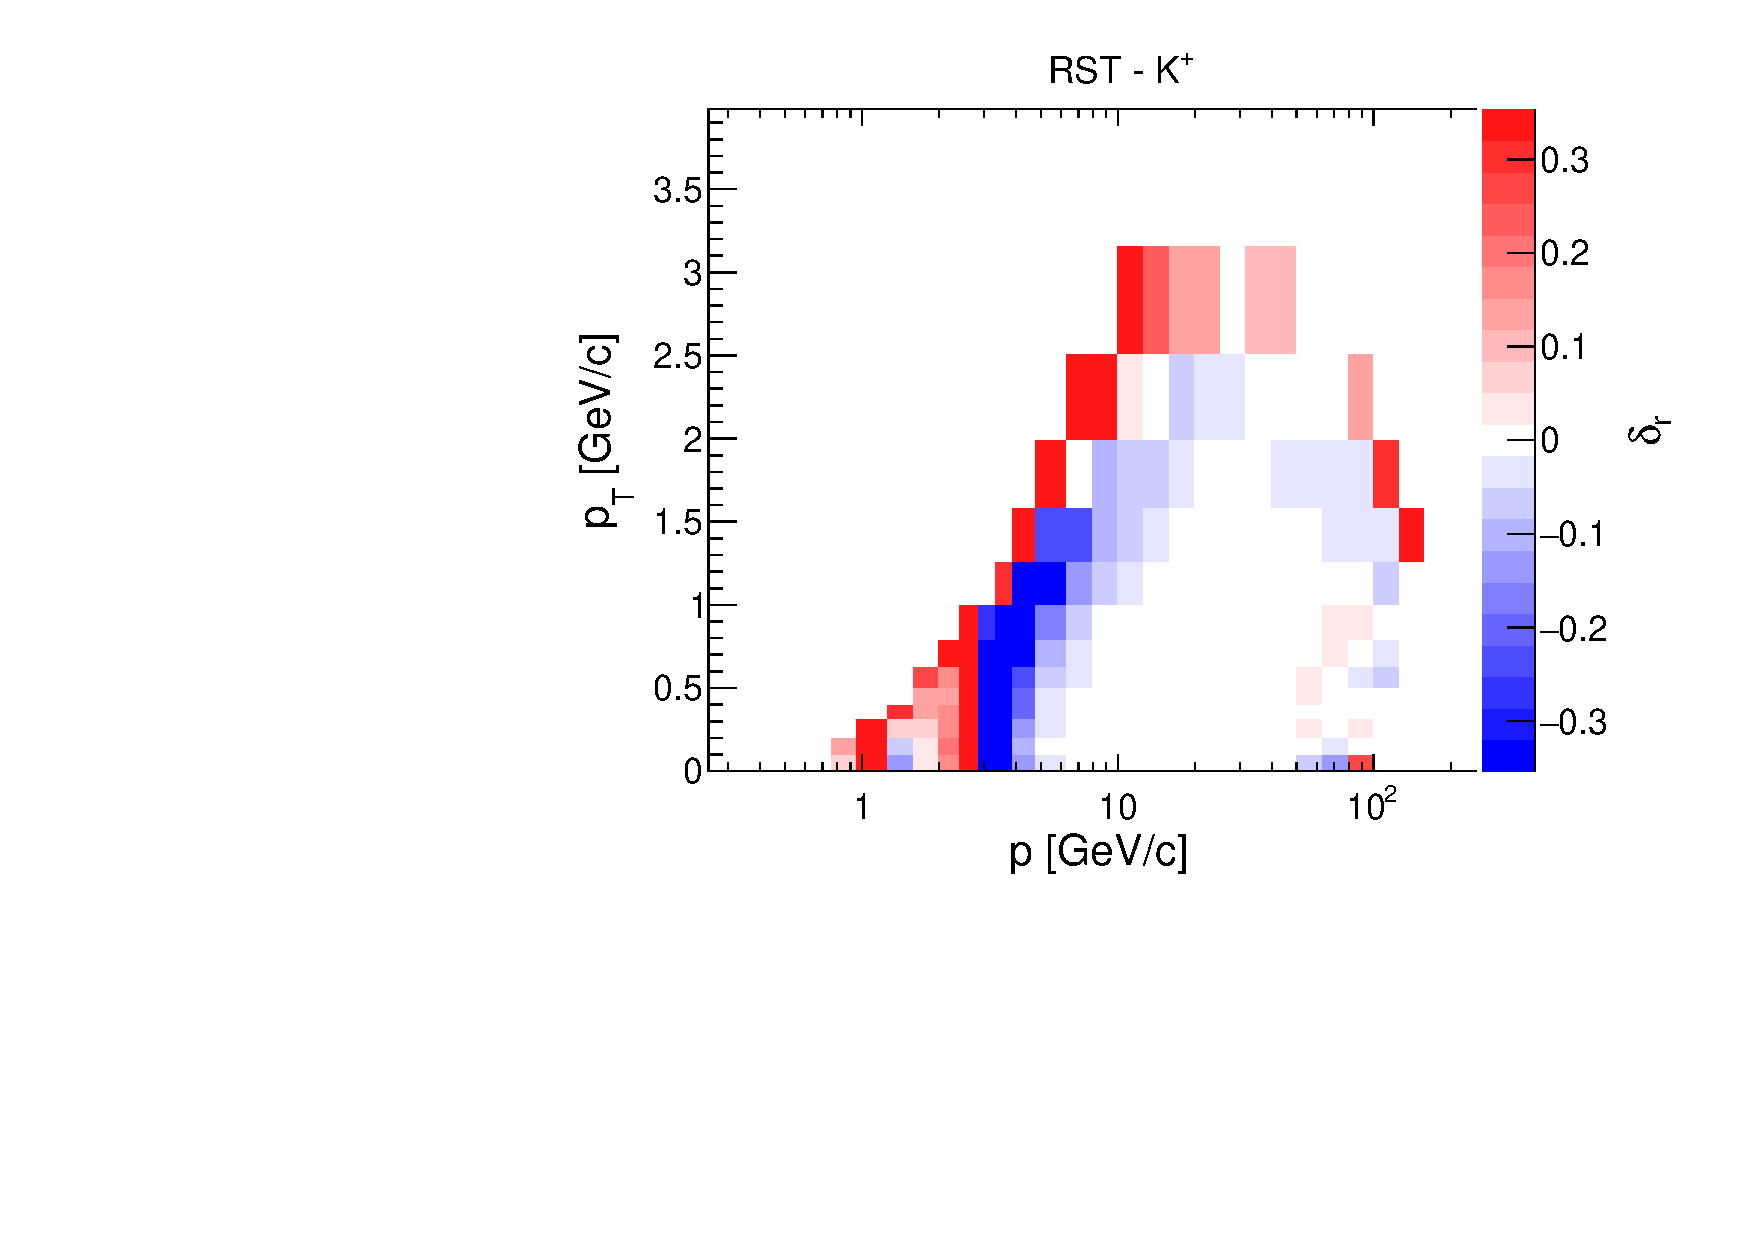
\includegraphics[clip, rviewport=0 0.13 1 0.94,width=0.4\textwidth]{dedx/fake_rel_dev_158_fl0_v0_c1_p2}

  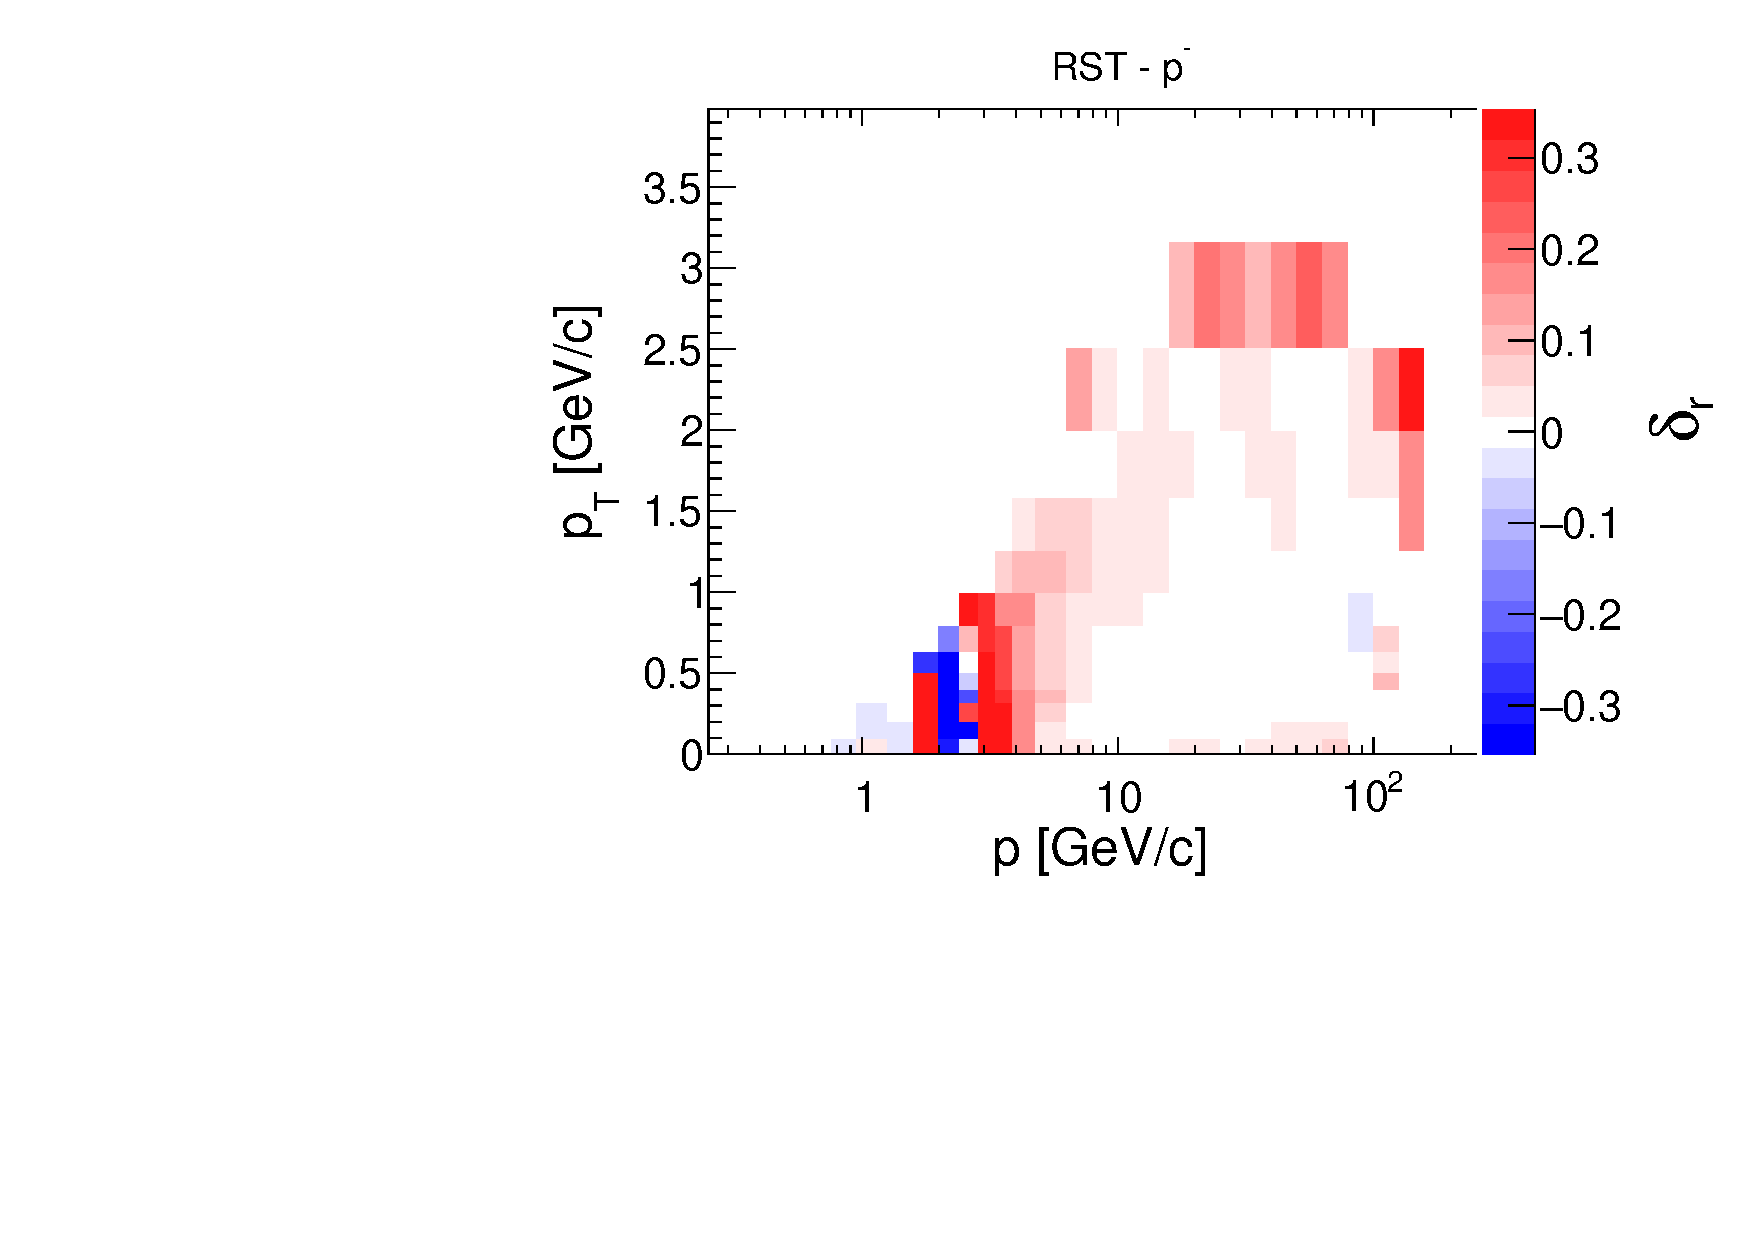
\includegraphics[clip, rviewport=0 0 1 0.94,width=0.4\textwidth]{dedx/fake_rel_dev_158_fl0_v0_c0_p3}
  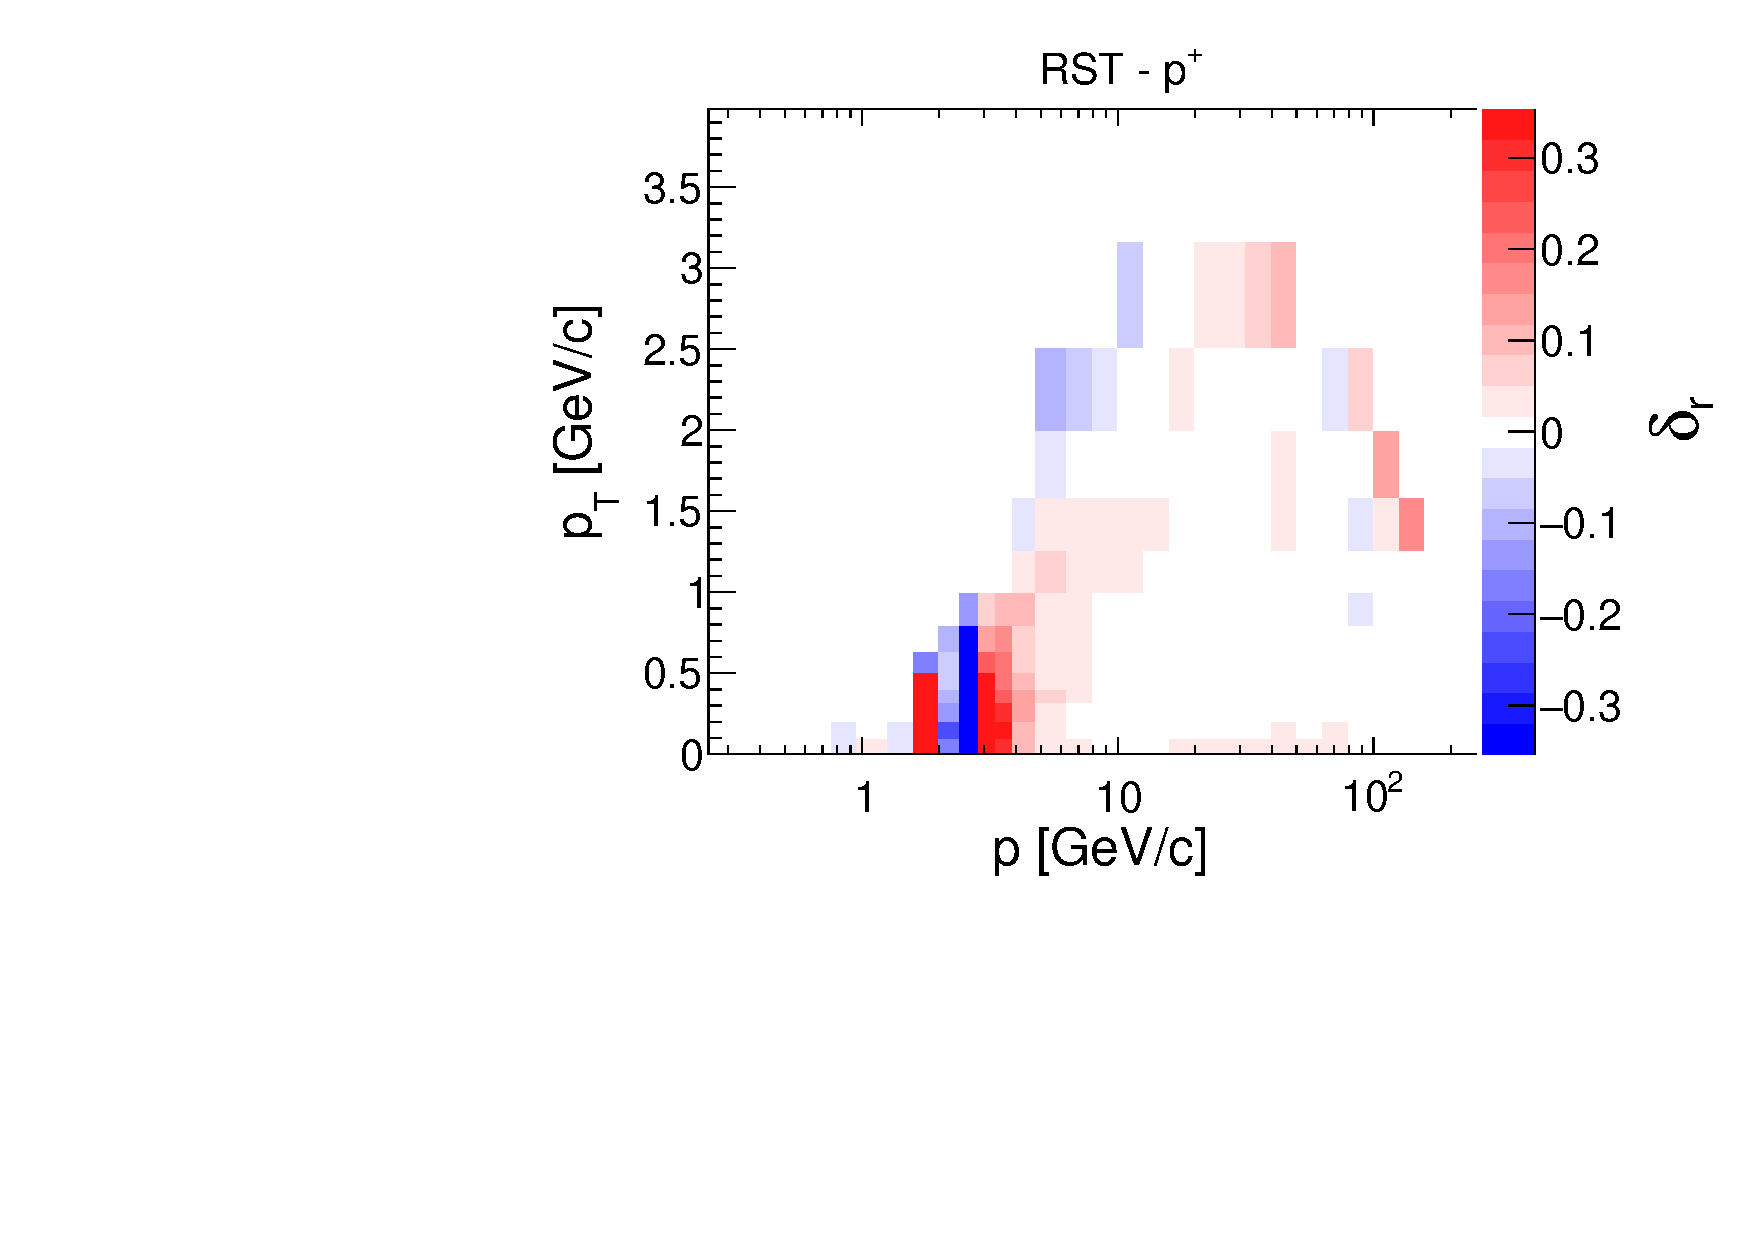
\includegraphics[clip, rviewport=0 0 1 0.94,width=0.4\textwidth]{dedx/fake_rel_dev_158_fl0_v0_c1_p3}


  \caption{Average relative bias of the particle fractions obtained with SDEs for RST and 158 \GeVc dataset.}
  \label{fig:hadron:dedx:fit:fake:reldev158r}
\end{figure}

From the $\sigma_r$ one can clearly see
that for few \pp bins, mainly between 1 and 10 \GeVc,
the fitted fractions present a very large relative
standard deviation in comparison to the remaning phase space regions.
This is because of the proximity between the mean of the
\dedx distribution of two particle types that cause
a partial degeneracy between their fractions. The result
of the \dedx fit at these phase space bins are evidently not
suitable and because of that they will be removed from our analysis.
To this aim, the bins with $\sigma_r$ larger than 0.15 for \pions,
and 0.25 for \kaons and \protons were removed. 

From the $\delta_r$ we can observe that there are regions
of the phase space which presents a significant relative
bias on the fractions.
These regions are mainly the low statistic and the high \pp
bins. In the latter case, the fraction are biased because
the \dedx distributions of all particle types
approach to each other following the relativistic rise
behavior of the deposit energy function.
Attempts were made to eliminate this bias
by changing the fit strategy, however, we found no effective solution.
Therefore, we have decided for a correction procedure based on
the $\delta_r$ obtained from the SDEs.
The multiplicative correction factors is called $c$ and is shown
in~\cref{fig:hadron:dedx:fit:fake:cor158r} for the RST and 158 \GeVc case,
while the remaning cases are shown
in~\cref{fig:hadron:dedx:fit:fake:cor158w,fig:hadron:dedx:fit:fake:cor350r,fig:hadron:dedx:fit:fake:cor350w}.
The phase space bins removed the criteria described above are shown
as white bins.

Besides the cuts and corrections, the SDEs can also
be used to compute the statistical uncertainties of the particle fractions.
This was one by computing the standard deviation of
fractions obtained from the SDEs.


%The fit performance can be studied by means of the
%pull distributions of the particle fractions.
%In~\cref{}

\note{pull distributions?}

\note{discussions here}

%%%%%%%%%% COR %%%%%%%%%%%%%%
\begin{figure}[!ht]
  \centering
  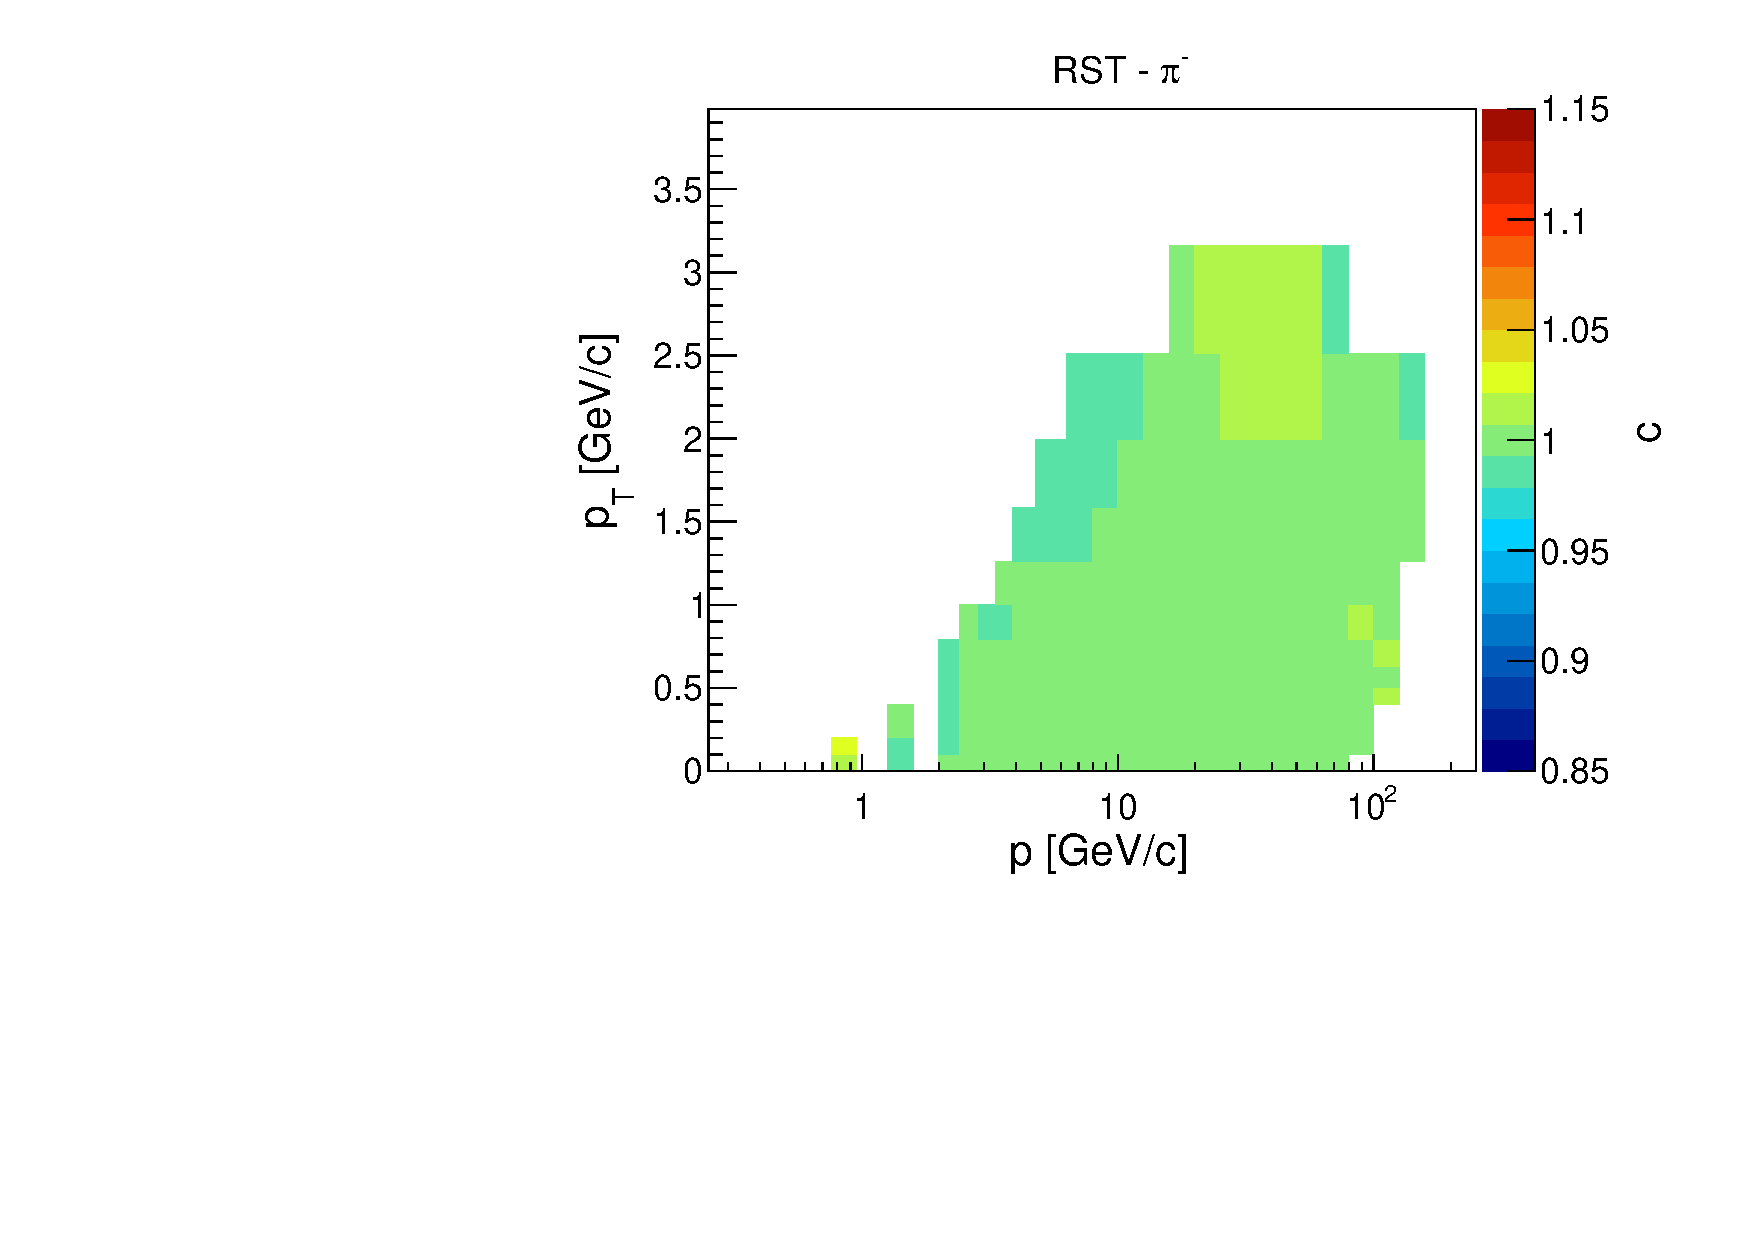
\includegraphics[clip, rviewport=0 0.13 1 0.94,width=0.4\textwidth]{dedx/cor_158_v0_c0_p1}
  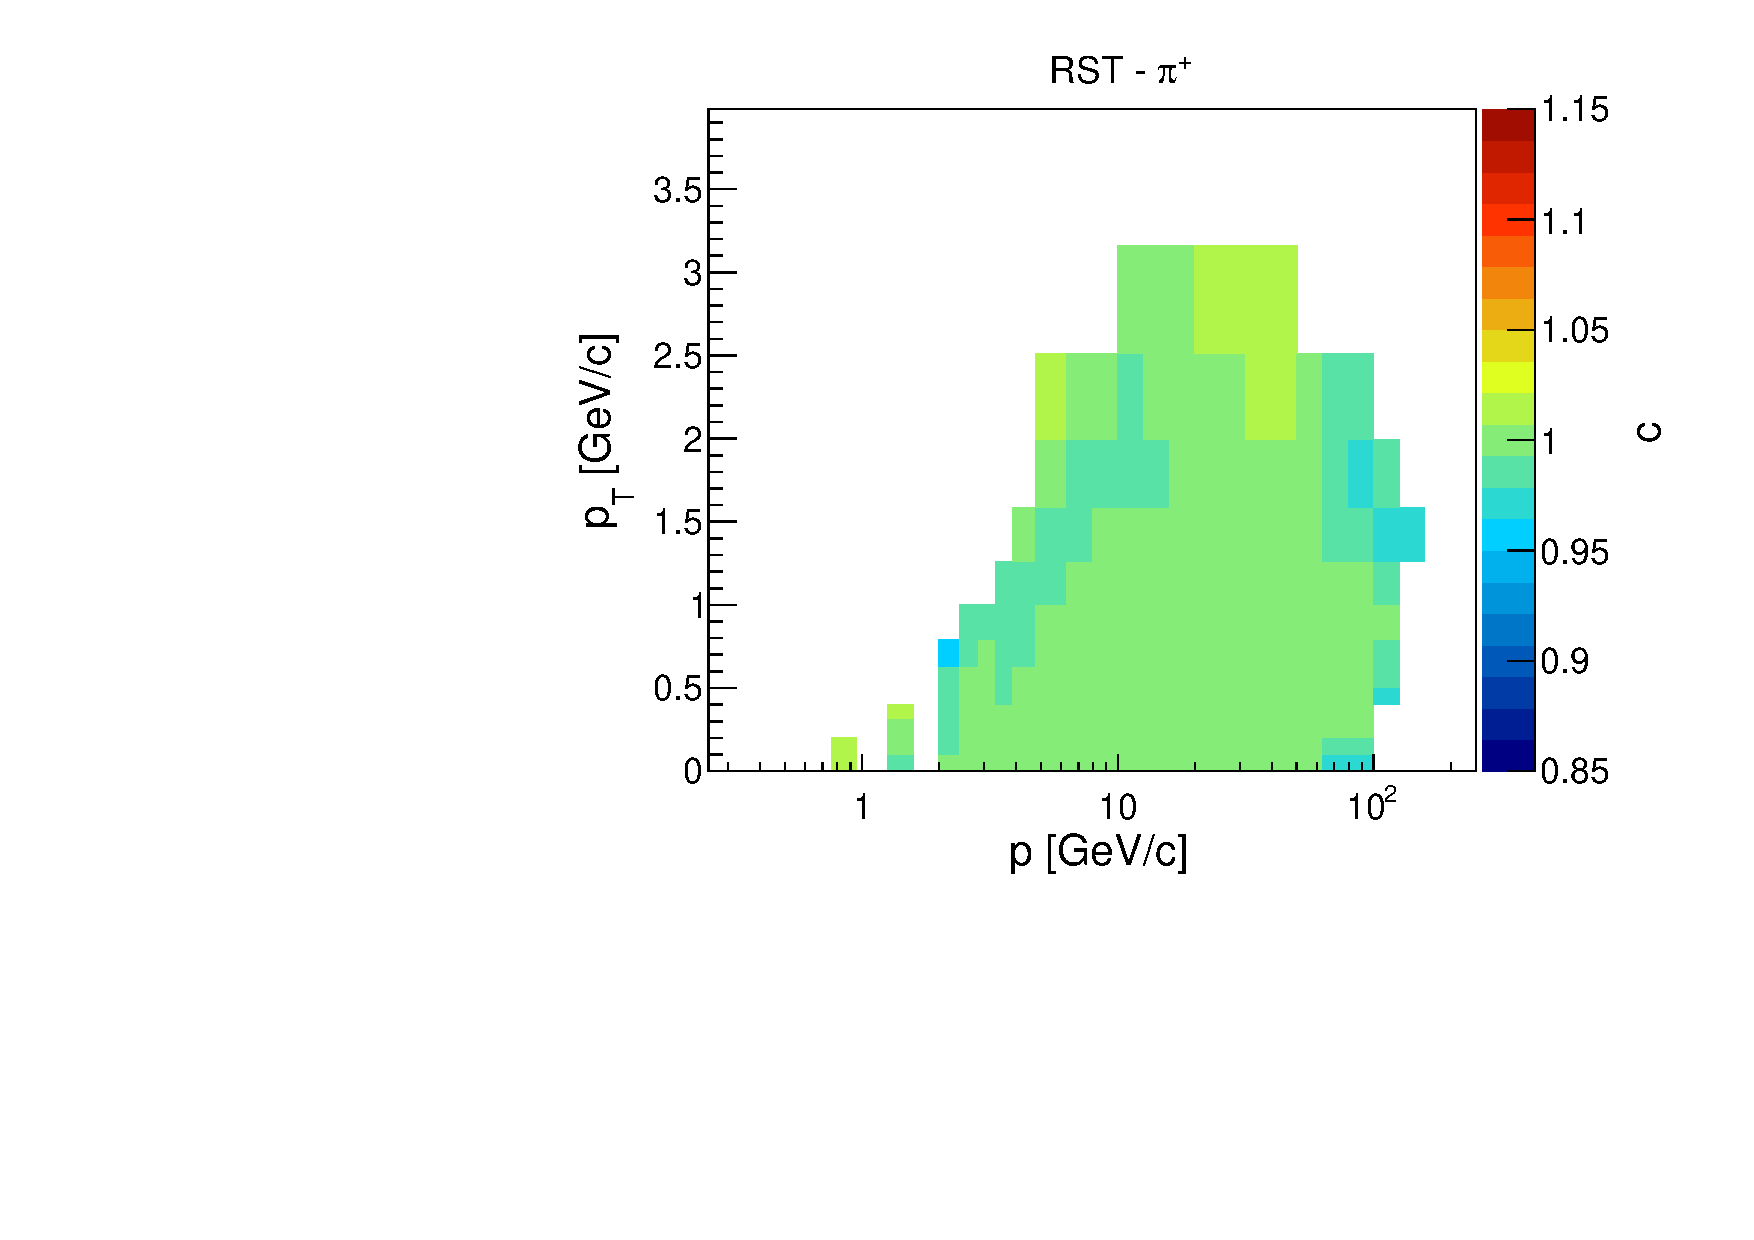
\includegraphics[clip, rviewport=0 0.13 1 0.94,width=0.4\textwidth]{dedx/cor_158_v0_c1_p1}

  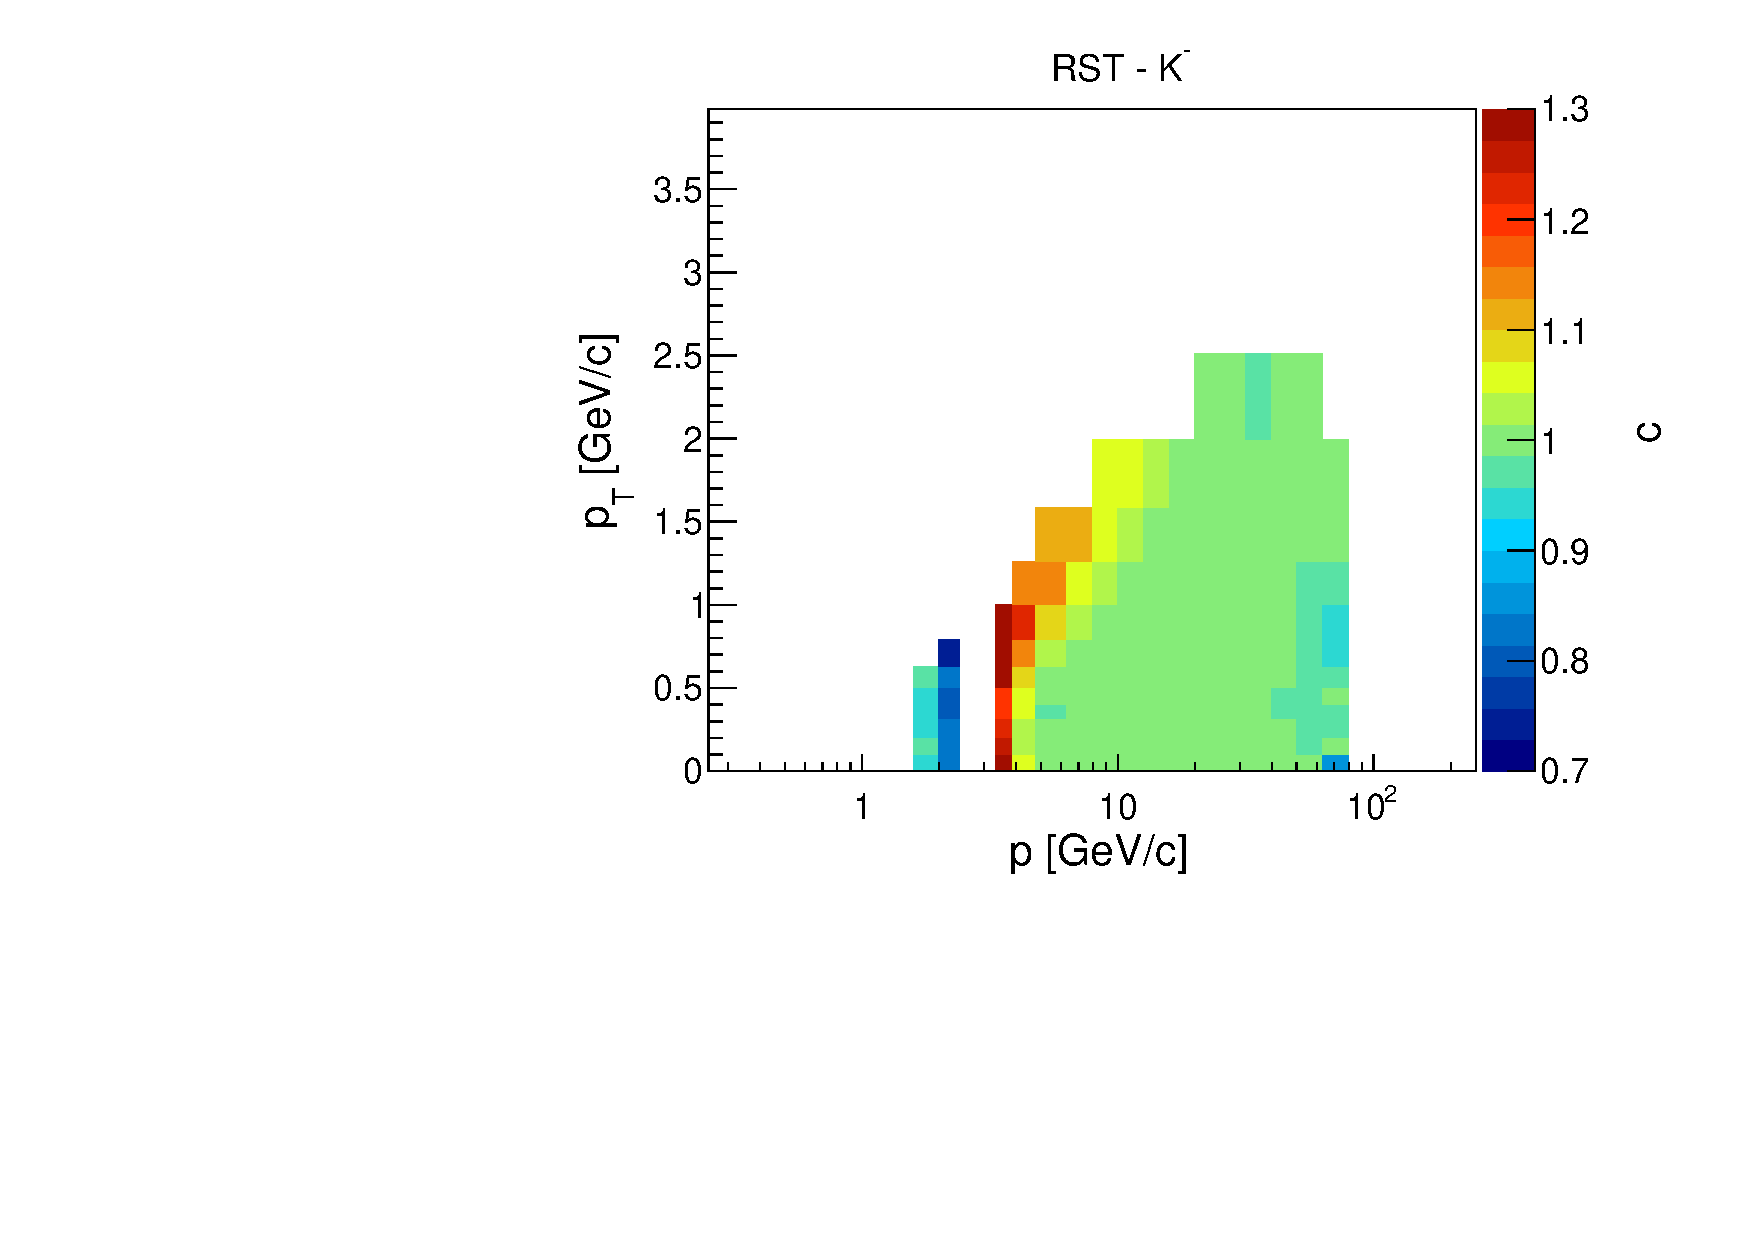
\includegraphics[clip, rviewport=0 0.13 1 0.94,width=0.4\textwidth]{dedx/cor_158_v0_c0_p2}
  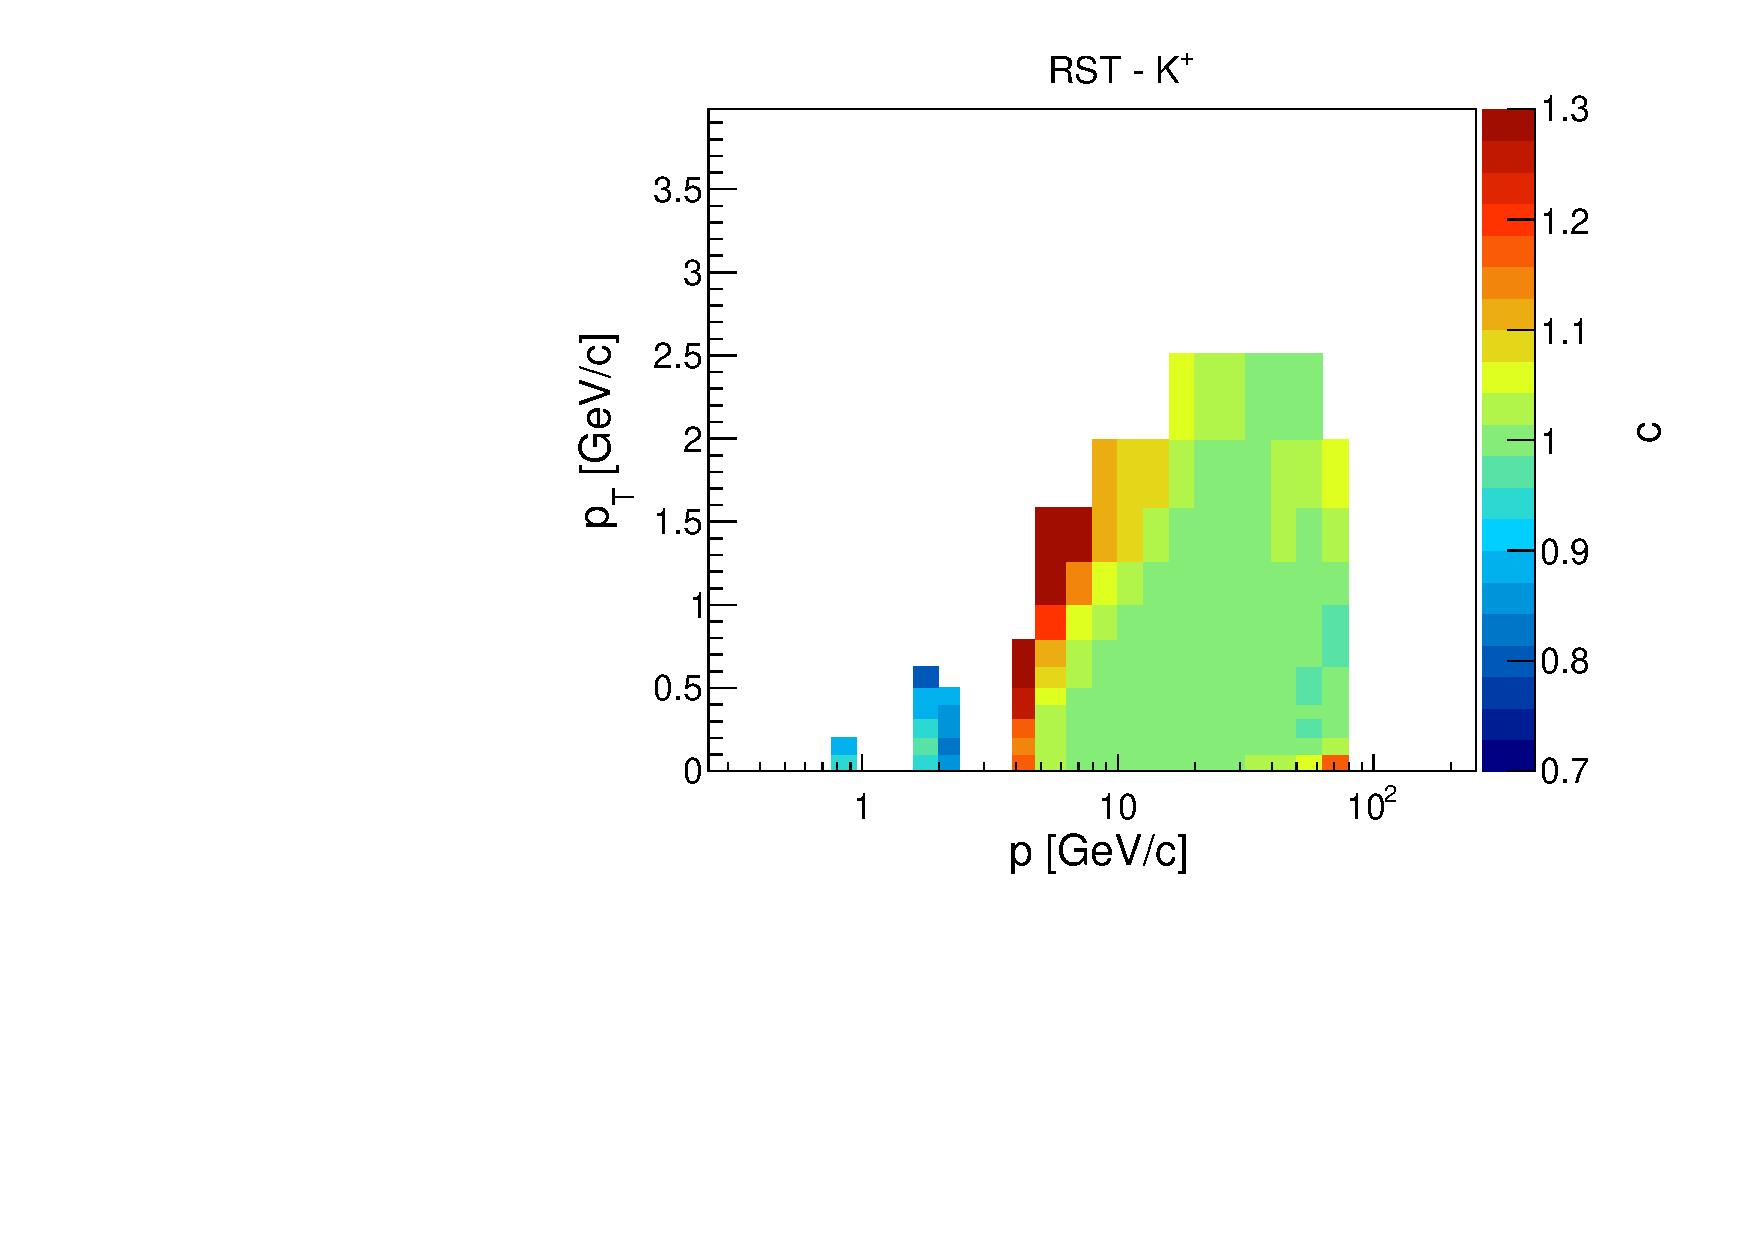
\includegraphics[clip, rviewport=0 0.13 1 0.94,width=0.4\textwidth]{dedx/cor_158_v0_c1_p2}

  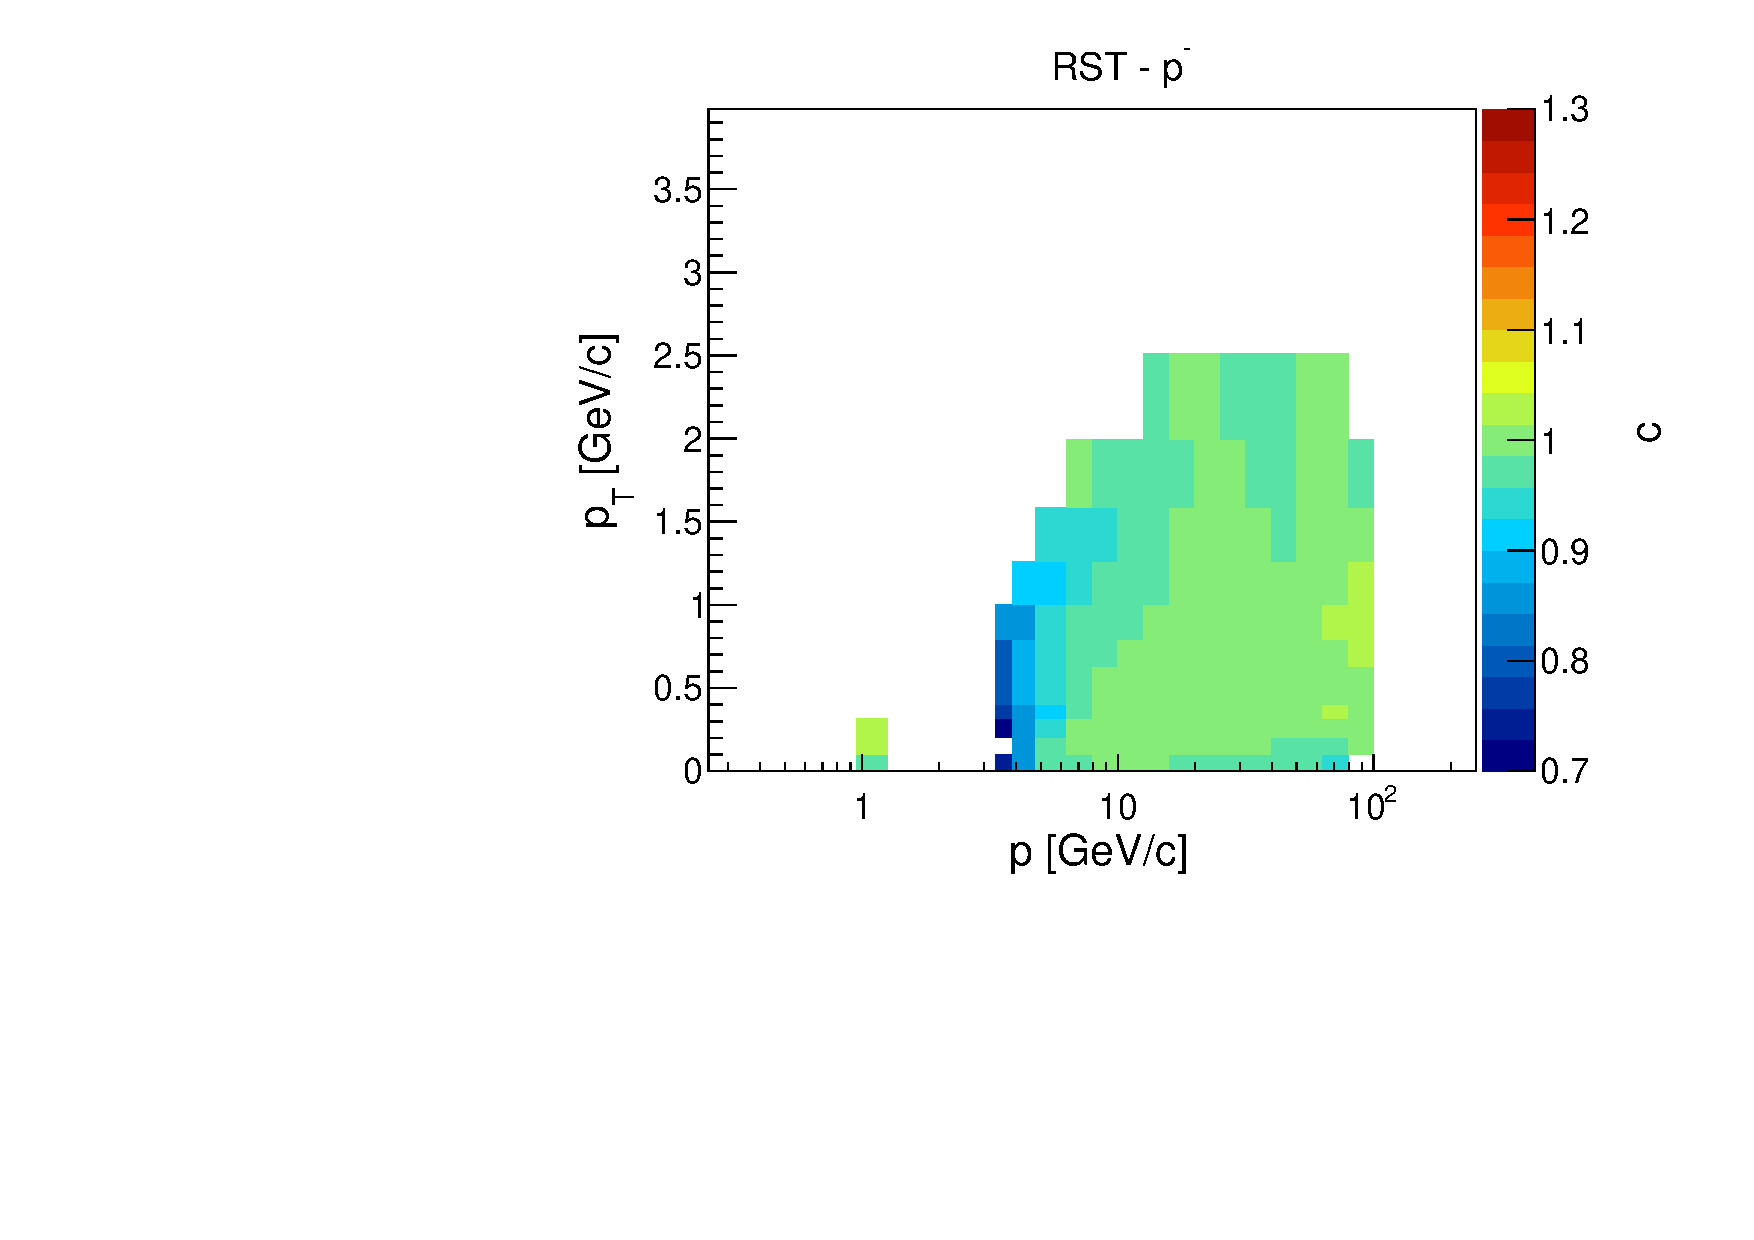
\includegraphics[clip, rviewport=0 0 1 0.94,width=0.4\textwidth]{dedx/cor_158_v0_c0_p3}
  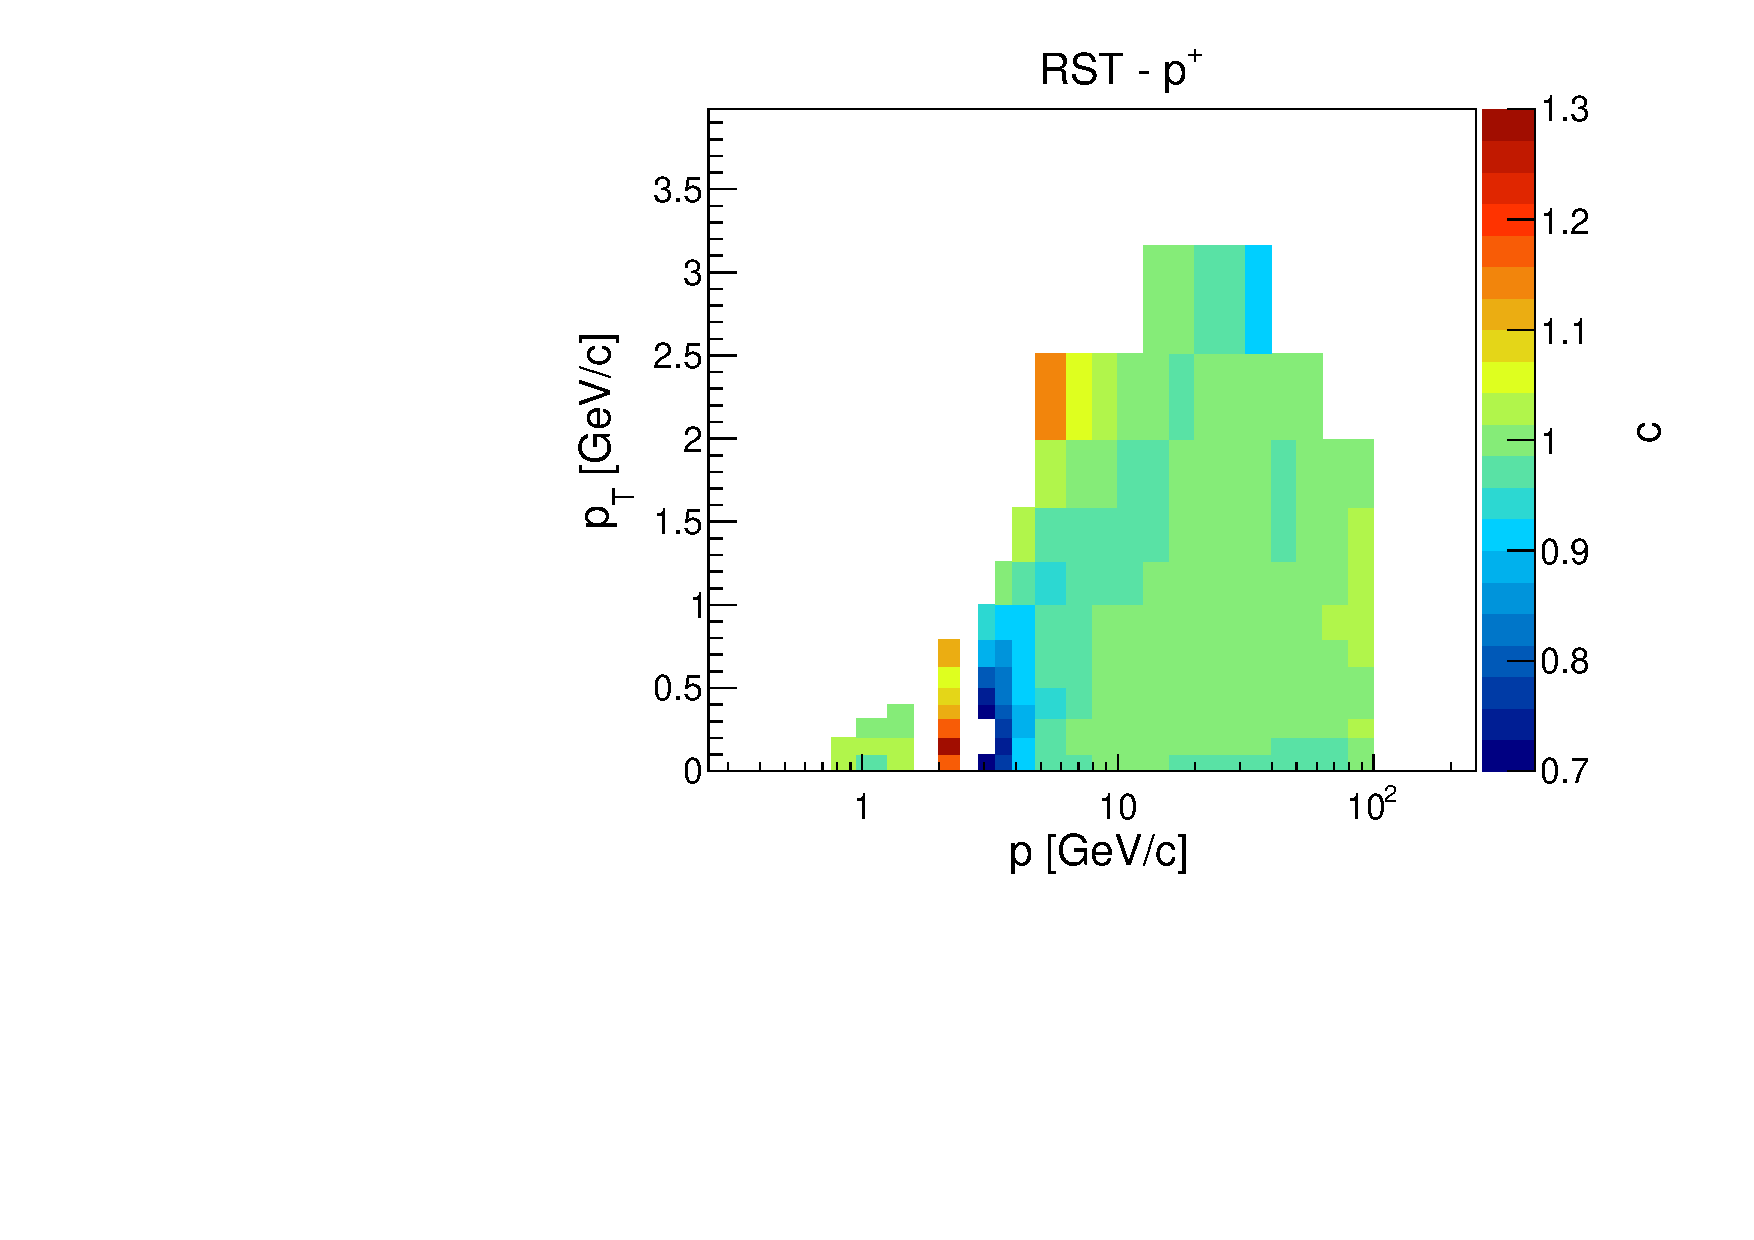
\includegraphics[clip, rviewport=0 0 1 0.94,width=0.4\textwidth]{dedx/cor_158_v0_c1_p3}

  \caption{Correction factor for RST and 158 \GeVc dataset.}
  \label{fig:hadron:dedx:fit:fake:cor158r}
\end{figure}


%%%---------------------------------%%%%
\subsection{Particle identification results}
\label{sec:hadron:dedx:results}

After applying the cuts and corrections discussed
in~\cref{sec:hadron:dedx:sde} we obtain the final
particle fractions to be used to compute the spectra.
In~\cref{fig:hadron:dedx:fit:final158r} we show examples
of the final fractions for RST and 158 \GeVc dataset,
while the remaning cases are shown 
in~\cref{fig:hadron:dedx:fit:final158w,fig:hadron:dedx:fit:final350r,fig:hadron:dedx:fit:final350w}.
Only the three particle types of interested are shown: $\pi$, $K$ and $p$.
Each plot shows the fractions as a function of \pp for one \pT bin.
The equivalent plots for the target removed dataset are shown
in~\cref{fig:hadron:dedx:fit:out158r,fig:hadron:dedx:fit:out158w,fig:hadron:dedx:fit:out350r,fig:hadron:dedx:fit:out350w}.

%%%%%%%%%% FRACTION %%%%%%%%%%%%%%
\begin{figure}
  \centering
  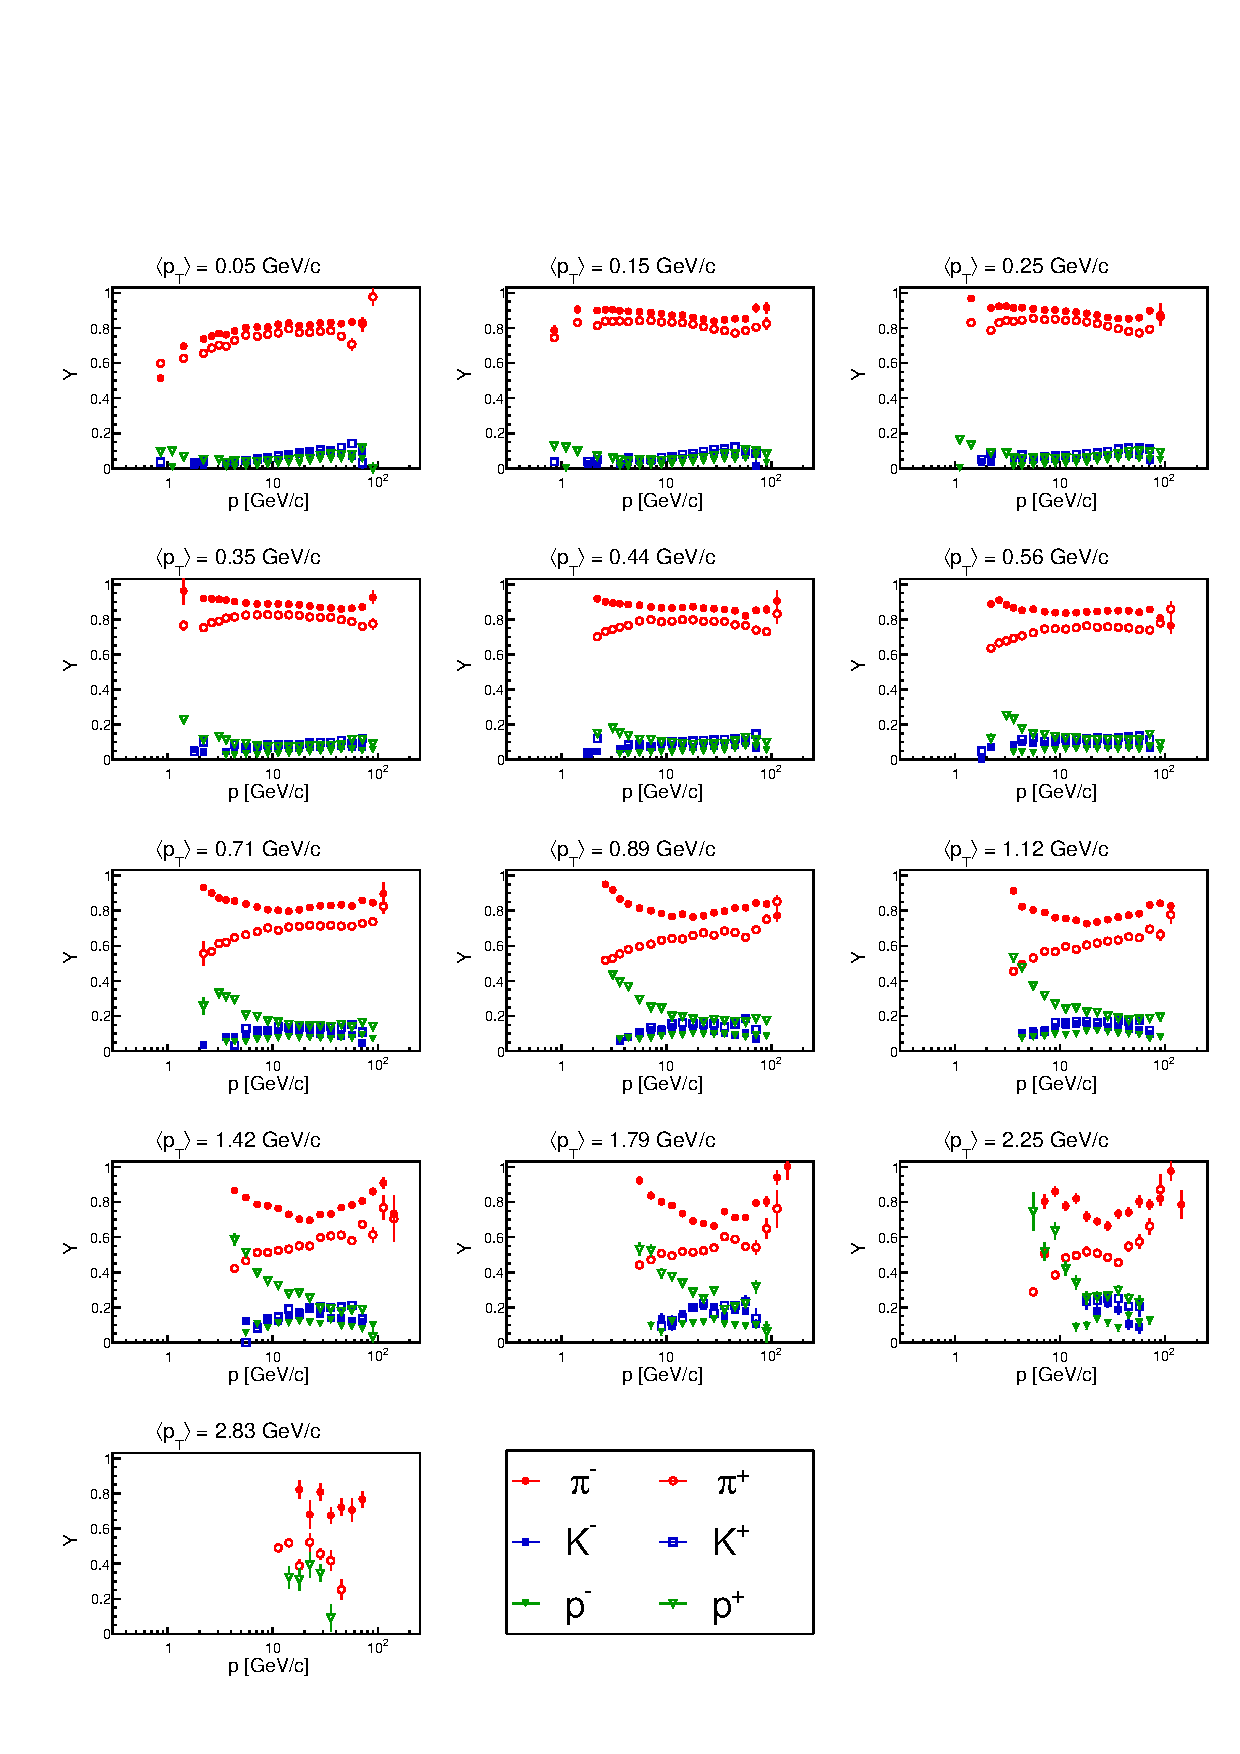
\includegraphics[clip, rviewport=0 0 1 1,width=1.00\textwidth]{dedx/fraction_pt_158_fl2_v0}
  \caption{Particle fractions obtained from the \dedx fit of the RST and 158 \GeVc dataset, with target inserted.}
  \label{fig:hadron:dedx:fit:final158r}
\end{figure}


%%%%%%%%%%%%%%%%%%%%%%%%%%%%%%%%%%%%%%%%
\section{\vzero analysis}
\label{sec:hadron:vzero}

In this section we describe the part of our analysis
focused on the \lambs and \kzeros particles.
Neutral weakly decaying particles with average decay length ($c\tau$)
of order of few or tens of centimeters can be detected by \NASixtyOne
experiment through their charged decay products. This kind of
particles are called \vzero particles because of the shape of
the decay ($V$) and its neutral charge ($^0$). Although the \vzero
particle itself does not create a track in the TPCs, the products
of its decay do, allowing us to reconstruct the position of the
decay vertex and, by using the properties of the daughter tracks,
identify the original \vzero. Therefore, the detector acceptance
depends strongly on geometrical factors because both daughter particles
must create tracks on the TPCs and they must be well reconstructed. 
In~\cref{tab:hadron:vzero:part} we list the three \vzero particles of interested
of the present work together with the properties of their decay channel
which is used here (daughter particles and branching ratio). 


\begin{table}
  \begin{center}
    \begin{tabular}{|c|c|c|} \hline
      \vzero particle  & decay products       & BR     \\ \hline
      \lamb            & \proton+$\pi^-$      & 63.9$\%$ \\ 
      \antilamb        & $\pi^+$+\antiproton  & 63.9$\%$  \\
      \kzeros          & $\pi^+$+$\pi^-$      & 69.2$\%$  \\ \hline
    \end{tabular}
    \caption{}
    \label{tab:hadron:vzero:part}
  \end{center}
\end{table}


The description of the standard algorithms applied by \NASixtyOne experiment
to find and reconstruct the \vzeros can be found in
Refs.~\cite{BarnaThesis,TobiaszThesis},
while the particular \vzero selection applied to our
analysis was described in~\cref{sec:hadron:vzeroselection}.
The identification of the \vzero particles is done by means of
its invariant mass, which is given by
\begin{equation}
  m_\text{inv} = \sqrt{m_+^2 + m_-^2 + 2(E_+E_--\vec{p}_+\vec{p}_-)},
\end{equation}
where the indexes $+$ and $-$ refer to the positively
and negatively charged daughter particles.
Because of the large combinatorial background, which means that
many tracks can be randomly combined and reconstructed as \vzero
particles, a signal extraction step is needed. This is usually done
by fitting the measured invariant mass distribution with a signal
and a background model. The signal extraction procedure is presented
in~\cref{sec:hadron:vzero:signal} and its results are shown
in~\cref{sec:hadron:vzero:results}.

%%%%%%%%%%%%%%%%%%%%%%%%%%%%%%%%%%%%%%%%
\subsection{\vzero selection}
\label{sec:hadron:vzero:selection}

\note{TO REVIEW}

The \vzero selection criteria used for the \vzero analysis
is the following:
\begin{enumerate}[label=(\roman*)]
\item The selected vertex must be identified as a \vzero type vertex.
\item The number of daughter tracks of the vertex must be equal to 2.
\item Both daughter tracks must be of opposite charges.
\item The total number of cluster has to be greater than 30 for both tracks
\item At least one track has to have more than 15 clusters in the VTPCs
\end{enumerate}
These selection criteria are standard ones in \NASixtyOne analysis.
Further cuts on the \vzeros will be applied at the signal extraction
step (see~\cref{sec:hadron:vzero:signal:cuts}).

Since it is not possible to define the detector acceptance for
the \vzeros analogously to what is done for the tracks, the possible
discrepancies between data and simulations on the borders of the acceptance
will be accounted on the systematic uncertainties (see~\cref{sec:hadron:spec:syst}).
Because these tracks on the borders have small number of clusters,
the systematic uncertainty will be estimated by changing the minimum number
of clusters on both tracks from 30 to 20. 

%%%---------------------------------%%%%
\subsection{Signal extraction strategy}
\label{sec:hadron:vzero:signal}


The signal extraction is done by fitting the \minv distribution
with a model that includes the signal and the background contributions.
Traditionally in \NASixtyOne analyzes the signal
is modelled by analytical functions like Breit-Wigner
or Gaussian functions~\cite{Abgrall:2015hmv,Aduszkiewicz:2015dmr}. 
However, because of difficulties in describing
the \kzeros signal, we have decided to use here
Monte Carlo templates instead. More than that, it was found
that for few \kzeros phase space bins,
the signal description is very poor
with only one single template and therefore a double template approach
was preferred.
The simulations used to build the templates were described
in~\cref{sec:hadron:data} and they include most of the expected
detector effects. It was observed that the choice of the
hadronic interaction model has an insignificant impact
on the shape of the templates.
For the background description we have decided
for the standard approach, using generic polynomial functions.



The fit is performed by a likelihood method assuming Poissonian
distributions for the entries of the \minv distribution.
The log-likelihood to be maximized is analogous to the one shown
in~\cref{eq:hadron:dedx:fit:l0}, however the notation is
simpler because the only index is the one
that refers to the \minv bin. This index will be represented by \imass,
the total number of \minv bin by \nmass and the value of \minv in the center
of the bin by $m_\imass$. Also, the expected value of the particle mass
is represented by $m_0$.
Thus, being $n$ and $\nu$ the observed and expected number, respectively,
the log-likelihood function is given by
\begin{equation}
  l_0 = 2\ln L = 2\sum_{\imass=1}^{\nmass} \left(\nu_{\imass} - n_{\imass}\ln\nu_{\imass}\right). 
  \label{eq:hadron:vzero:fit:l0}
\end{equation}
The expected number $\nu_\imass$ is given by the sum of the signal
and background contribution as
\begin{equation}
  \nu_\imass = T_\imass + f^\text{BG}_\imass, 
  \label{eq:hadron:vzero:fit:nu}
\end{equation}
where $T_\imass$ comes from the templates and
\begin{equation}
  f^\text{BG}_\imass = p_0 + p_1(m_\imass-m_0)+p_2(m_\imass-m_0)^2.
  \label{eq:hadron:vzero:fit:bg}
\end{equation}


The contribution of one template evaluated at a given
mass $m$ is represented by $t[m]$. The templates contain
the same number of bins \nmass and $t[m]$ is computed
by a linear interpolation of the two bins
in which their centers are the closest to $m$.
To allow the templates to shift, we added the
shift parameters $\delta m$'s. In the end,
the template term $T_\imass$ computed by
\begin{equation}
  T_\imass = S_\text{fit}\left(\alpha t^0[m_\imass+\Delta m^0]+ (1-\alpha)t^1[m_\imass+\Delta m^1]\right),
  \label{eq:hadron:vzero:fit:t}
\end{equation}
where $S_\text{fit}$, $\alpha$, $\Delta m^0$ and $\Delta m^1$ are
free parameters to be fitted.
Since the templates are normalized, $S_\text{fit}$ gives
directly the amount of signal in the distribution.

By combining the~\cref{eq:hadron:vzero:fit:nu,eq:hadron:vzero:fit:bg,eq:hadron:vzero:fit:t}
with~\cref{eq:hadron:vzero:fit:l0} we have the log-likelihood function $l_0$
with 7 free parameters, being $p_0$, $p_1$ and $p_2$
for the background and $S_\text{fit}$, $\alpha$, $\Delta m^0$ and $\Delta m^1$
for the signal.

Similarly to what was done for the \dedx fit,
here we also include Gaussian contraints to make the
fit more stable. The parameters to be contrained are
the mass shifts, $\Delta m^0$ and $\Delta m^1$, and the fraction
$\alpha$. In the former case the intentional is to avoid
solutions of the fit in which the template shifts are too large.
It is expected shifts of order of few \MeVc only and it was observed
that without the contraints there could be solutions with
larger shift than this, which is physically meaningless.
The contraint on the $\alpha$ parameter is important
for cases in which the signal is well described by one
template only and consequently $\alpha$ becomes
degenerated. The contraint term is given by
\begin{equation}
  c = \left(\frac{\Delta m^0}{0.001}\right)^2+\left(\frac{\Delta m^1}{0.003}\right)^2
  +\left(\frac{\alpha}{0.2}\right)^2,
  \label{eq:hadron:vzero:fit:c}
\end{equation}
where the $\Delta m^0$ and $\Delta m^1$ is given in \GeVc units.
Finally, the final log-likelihood to be maximized is given by
\begin{equation}
  l = l_0 +c,
  \label{eq:hadron:vzero:fit:l}
\end{equation}
where $l_0$ and $c$ are given by~\cref{eq:hadron:vzero:fit:l}
and~\cref{eq:hadron:vzero:fit:c}, respectively.

The maximization of $l$ was done by means of the
MINUIT package~\cite{James:1975dr}. The width
of the \minv bins was 1.5 and 3.0 \MeVcc for
\lambs and \kzeros, respectively, and the mass range
was $[1.095 \GeVcc, 1.160 \GeVcc]$ and $[0.42 \GeVcc, 0.580 \GeVcc]$  
again for \lambs and \kzeros, respectively.
For each beam energy dataset, the templates were filled
with the three simulation sets, generated by different
hadronic interaction models.

As results of the fit, we obtain the estimated signal
$S_\text{fit}$, and the average background $B_\text{fit}$, which is the integral
of the background function over all the mass range of the fit.
To avoid possible bias due to misdescription of the signal
by the templates, the final signal is not taken as $S_\text{fit}$.
Instead, we compute it as $S = N - B_\text{fit}$,
where $N$ is the total number of entries in the measured \minv distribution.
We assume by doing this that the background estimation is more precise
than the signal one.
The statistical uncertainty on $S$ is given by $\sigma_S = \sqrt{N+\sigma_{B_\text{fit}}^2}$,
where Poissonian fluctuations are assumed for $N$ and $\sigma_{B_\text{fit}}$
is obtained as a result of the fit.

To determine suitable starting parameters for the fit,
a preliminary phase is performed by means of a $\chi^2$
fit. In this case, the signal model is simplified and
only one template is used without allowing it to shift.
In this way the whole model turns to be linear on the fitting
parameters and the $\chi^2$ minimization can be done annalytically.
The results of the $\chi^2$ fit
is then used to compute the respective parameters
to start the final fit.

Because the number of selected \vzeros is substantially smaller
at the target removed dataset, a special strategy for the signal
extraction is required. First, the phase space binning was
changed so all the original \pT bins are merged
in one unique bin for each \pp bin. Second, the \minv fit is performed
by means of an analytic minimization of the $\chi^2$
in which only one template is considered, without allowing
its position to shift. Although it is known that this fitting
procedure can produce biased results, it is acceptable in this
context because the statistical uncertainties due to the low
statistics is surely much larger than the bias.
After obtaining $S$ from the \minv fit, the target removed
signal for each original \pp and \pT bin is obtained by assuming
the same \pT dependence observed in the target inserted dataset.


%%%---------------------------------%%%%
\subsection{\vzero cuts}
\label{sec:hadron:vzero:signal:cuts}


The \vzero cuts are applied to the \minv data to reduce
the relative amount of background events, which
increases the precision of the signal extraction. 
Two quantities are used here for the \vzero cuts,
the radial impact parameter of the \vzero particle (\impact)
and its decay distance (\decaydist). The \impact is defined
as $\impact = \sqrt{(0.5b_x)^2+b_y^2}$, where $b_x$ and
$b_y$ are the coordinates $x$ and $y$ of the projection of \vzero particle
trajectory at the target plane. The factor 0.5 on $b_x$ is included
because the spread of $b_x$ is approximately 2 times larger than $b_y$.
In~\cref{fig:hadron:vzero:cuts:impact}
we show the \impact distribution for signal and background
obtained from simulations for all the phase space bins.
We can observe that the \impact parameter of signal \vzeros
are more concentrated at small values while the background ones
show a longer tale. Because of that, only \vzeros with \impact
small than a certain value were used for the signal extraction.
This value was chosen to be 2 cm. The efficiency of this cut
was observed to be larger than 90\% for all the phase space bins.

%%%%%%%%%%% IMPACT CUT %%%%%%%%%%%%
\begin{figure}
  \centering
  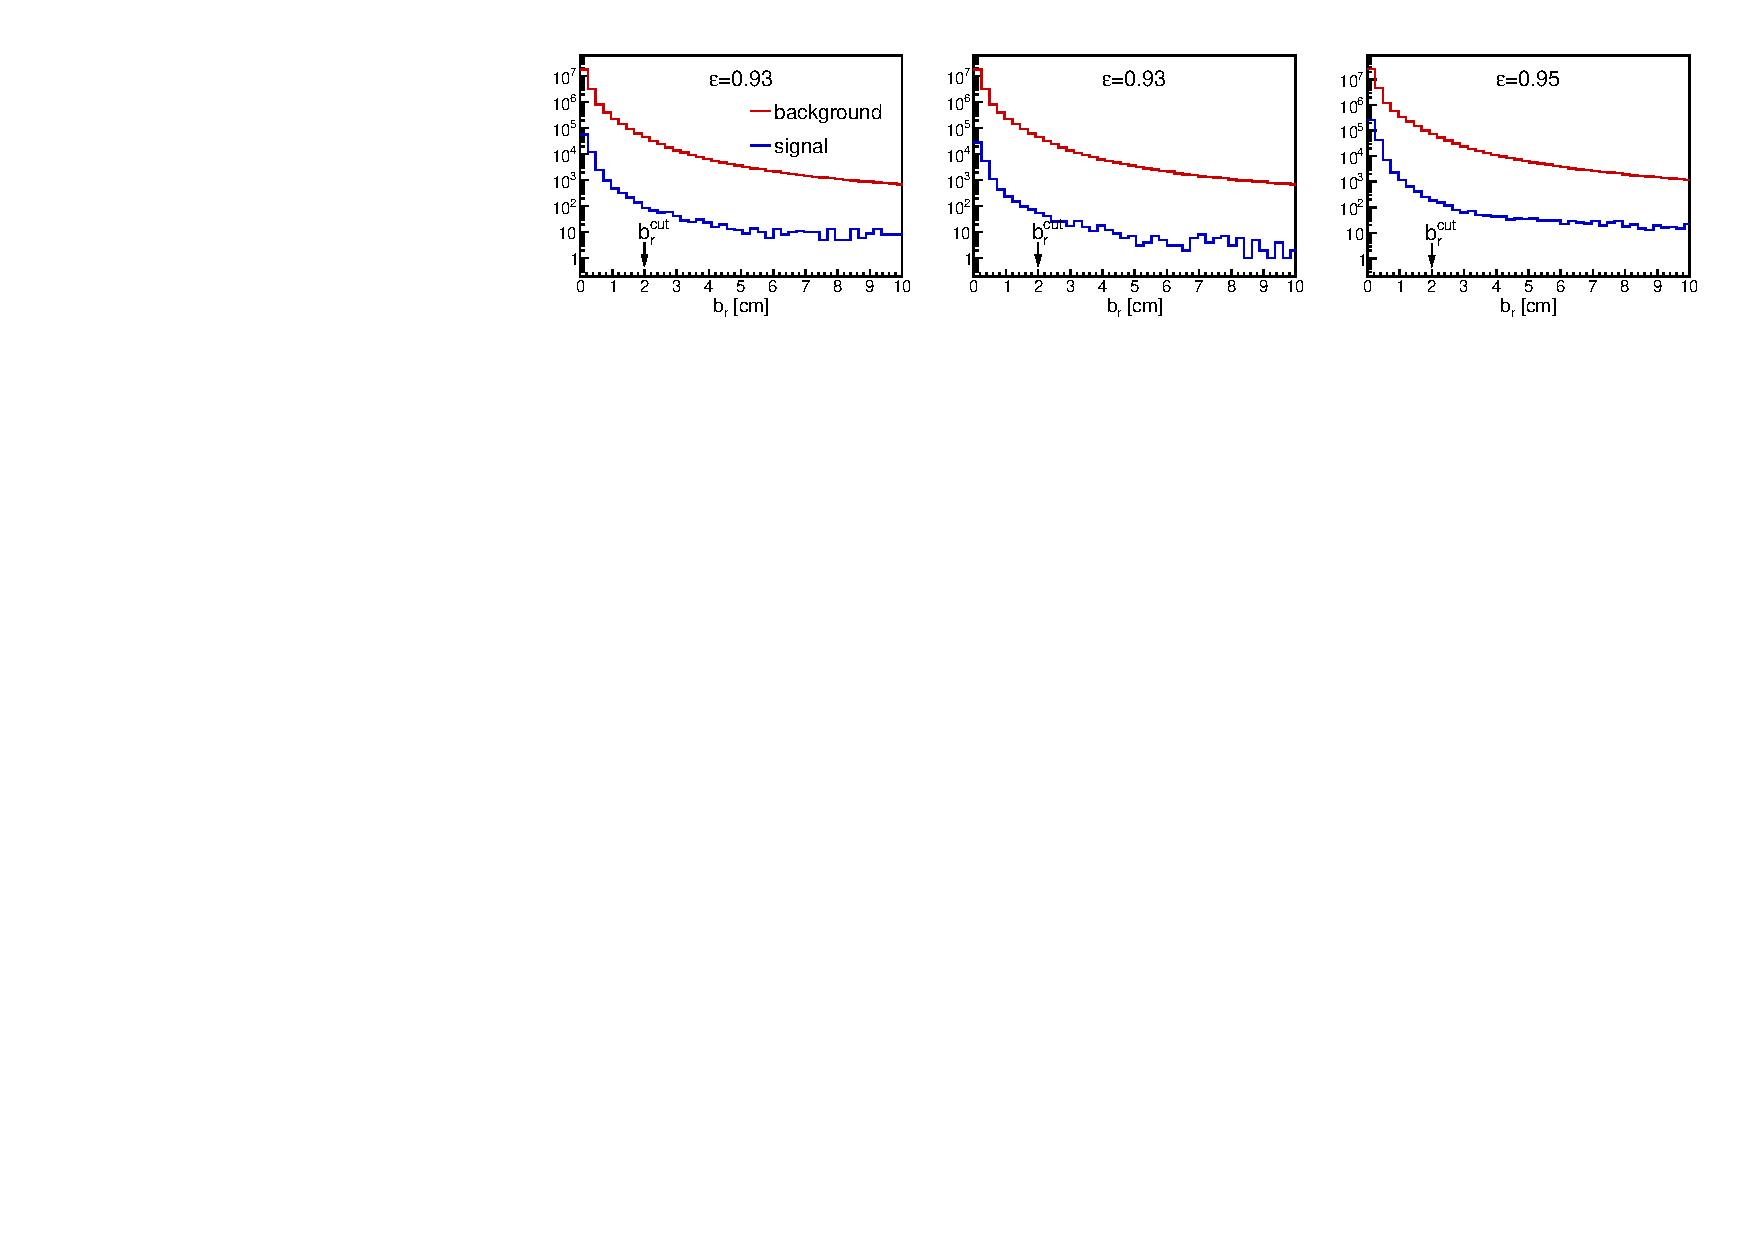
\includegraphics[clip, rviewport=0 0 1 1,width=0.99\textwidth]{vzero/cut_impact_all_SimEPOS158}
  
  \caption{}
  \label{fig:hadron:vzero:cuts:impact}
\end{figure}

The \decaydist is defined as the distance between the position
of the \vzero and the position of the main vertex.
The background \vzeros tend to have smaller \decaydist than
the signal ones, so \vzero with \decaydist
smaller than a given cut value \decaydistmin are removed.
Because of the physical dependence of the \decaydist with
the momentum of the particle, \decaydistmin was assumed to
depend on the \vzero momentum and it was optimized to minimize
the statistical uncertainty of the extracted signal.
The optimization was done by first performing the \minv fit
with many values of \decaydistmin and then evaluating
$S* = S/\varepsilon$ and its uncertainty $\sigma_{S*}$,
where $\varepsilon$ is the efficiency due to the \vzero cuts.
Next we found value of \decaydistmin that minimizes the
relative uncertainty $\sigma_{S*}/S*$, which is denoted by \decaydistopt.
One example of $\sigma_{S*}/S*$ as a function of \decaydistmin is
shown in~\cref{fig:hadron:vzero:cuts:decaydist:example}, where \decaydistopt is indicated.
The \decaydistopt found for all the phase space bins
are shown in~\cref{fig:hadron:vzero:cuts:decaydist:158,fig:hadron:vzero:cuts:decaydist:350}
as a function of the \vzero momemtum
where the average over the \pT bins are shown as red markers.
A fit of a linear function of $\log \pp$ to the average \decaydistopt
is shown as a red curve. Since this function shows to describe
in first order the momentum dependence of \decaydistopt,
we have decided to use it to define the \decaydistmin.

%%%%%%%%%%% DECAY DIST CUT EXAMPLE %%%%%%%%%%%%
\begin{figure}
  \centering
  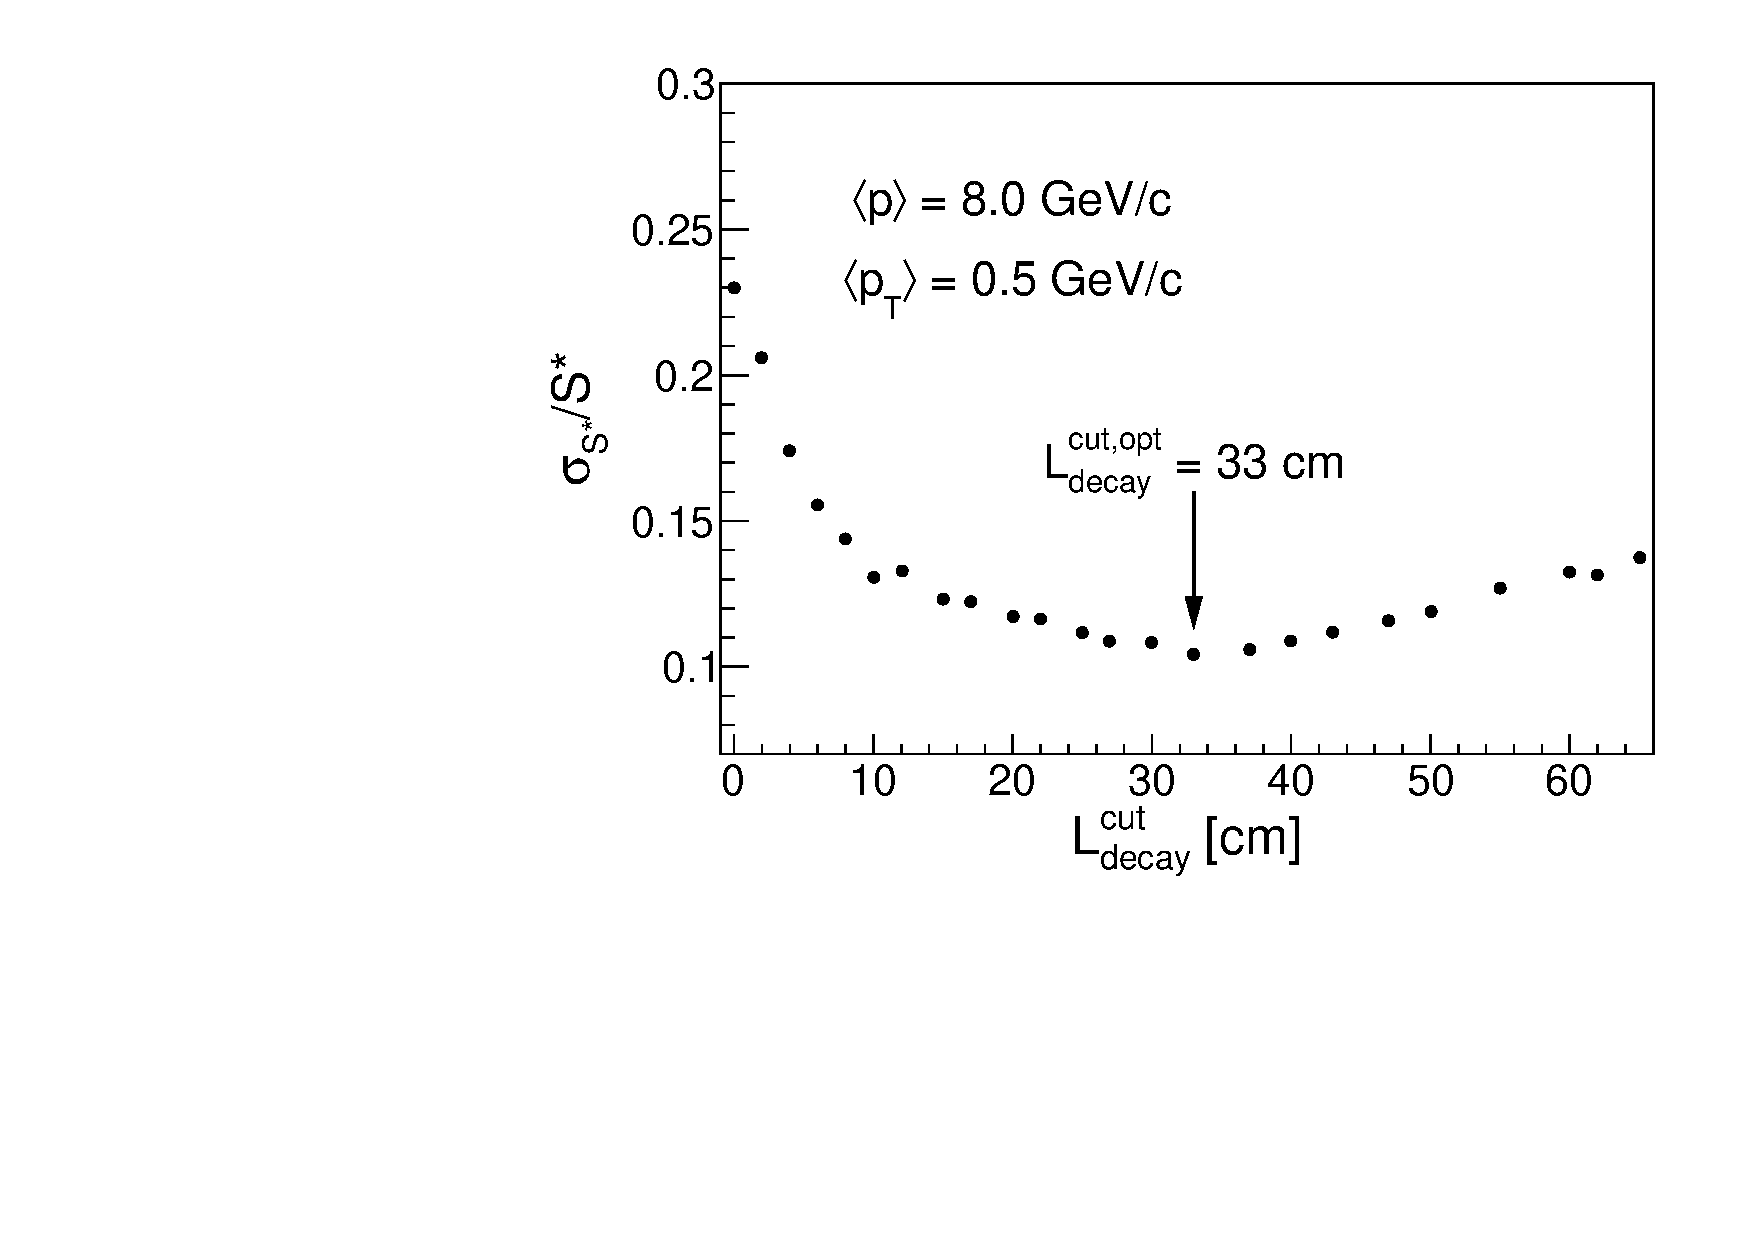
\includegraphics[clip, rviewport=0 0 1 1,width=0.65\textwidth]{vzero/cut_opt_350}
  
  \caption{}
  \label{fig:hadron:vzero:cuts:decaydist:example}
\end{figure}

%%%%%%%%%%% DECAY DIST CUT %%%%%%%%%%%%%%%%%%
\begin{figure}
  \centering
  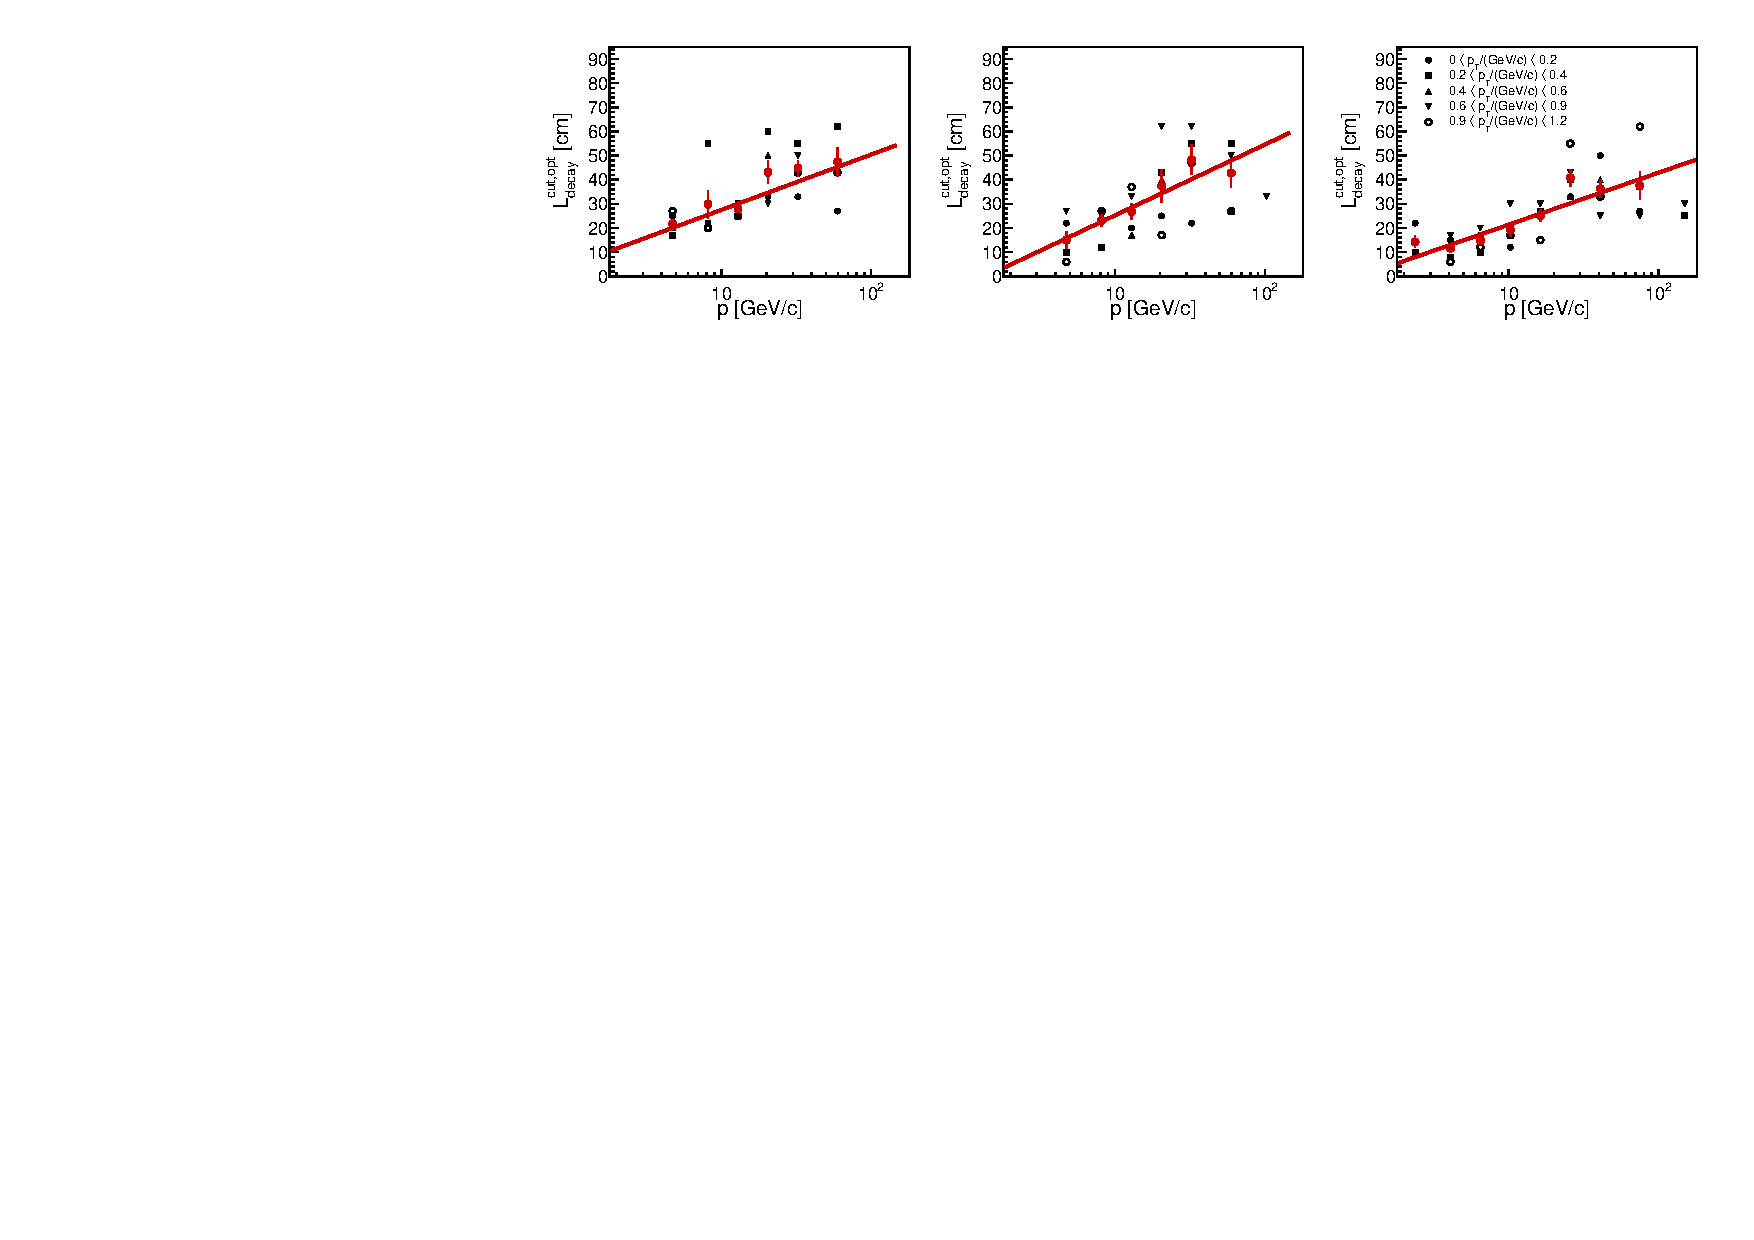
\includegraphics[clip, rviewport=0 0 1 1,width=0.99\textwidth]{vzero/cut_dist_Data158}
  
  \caption{Optimization of the \decaydistmin for the 158 \GeVc dataset. The plot on left, middle and right shows \lamb, \antilamb and \kzeros, respectively.}
  \label{fig:hadron:vzero:cuts:decaydist:158}
\end{figure}

The signal extraction described in~\cref{sec:hadron:vzero:signal}
was performed using the \minv distributions obtained
after appling both \vzero cuts described above.
The lost of signal \vzeros due to these cuts were corrected
at the Monte Carlo correction step, described in~\cref{sec:hadron:correction}.

%%%---------------------------------%%%%
\subsection{Signal extraction results}
\label{sec:hadron:vzero:results}

\note{TO REVIEW}

In~\cref{fig:hadron:vzero:signal:dist:158:in,fig:hadron:vzero:signal:dist:350:in}
we show examples of the fitted \minv distributions
for the target inserted dataset and
in~\cref{fig:hadron:vzero:signal:dist:158:out,fig:hadron:vzero:signal:dist:350:out}
for the target removed one.


%%%%%%%%%%% DIST %%%%%%%%%%%%%%%%%%
\begin{figure}[!ht]
  \centering
  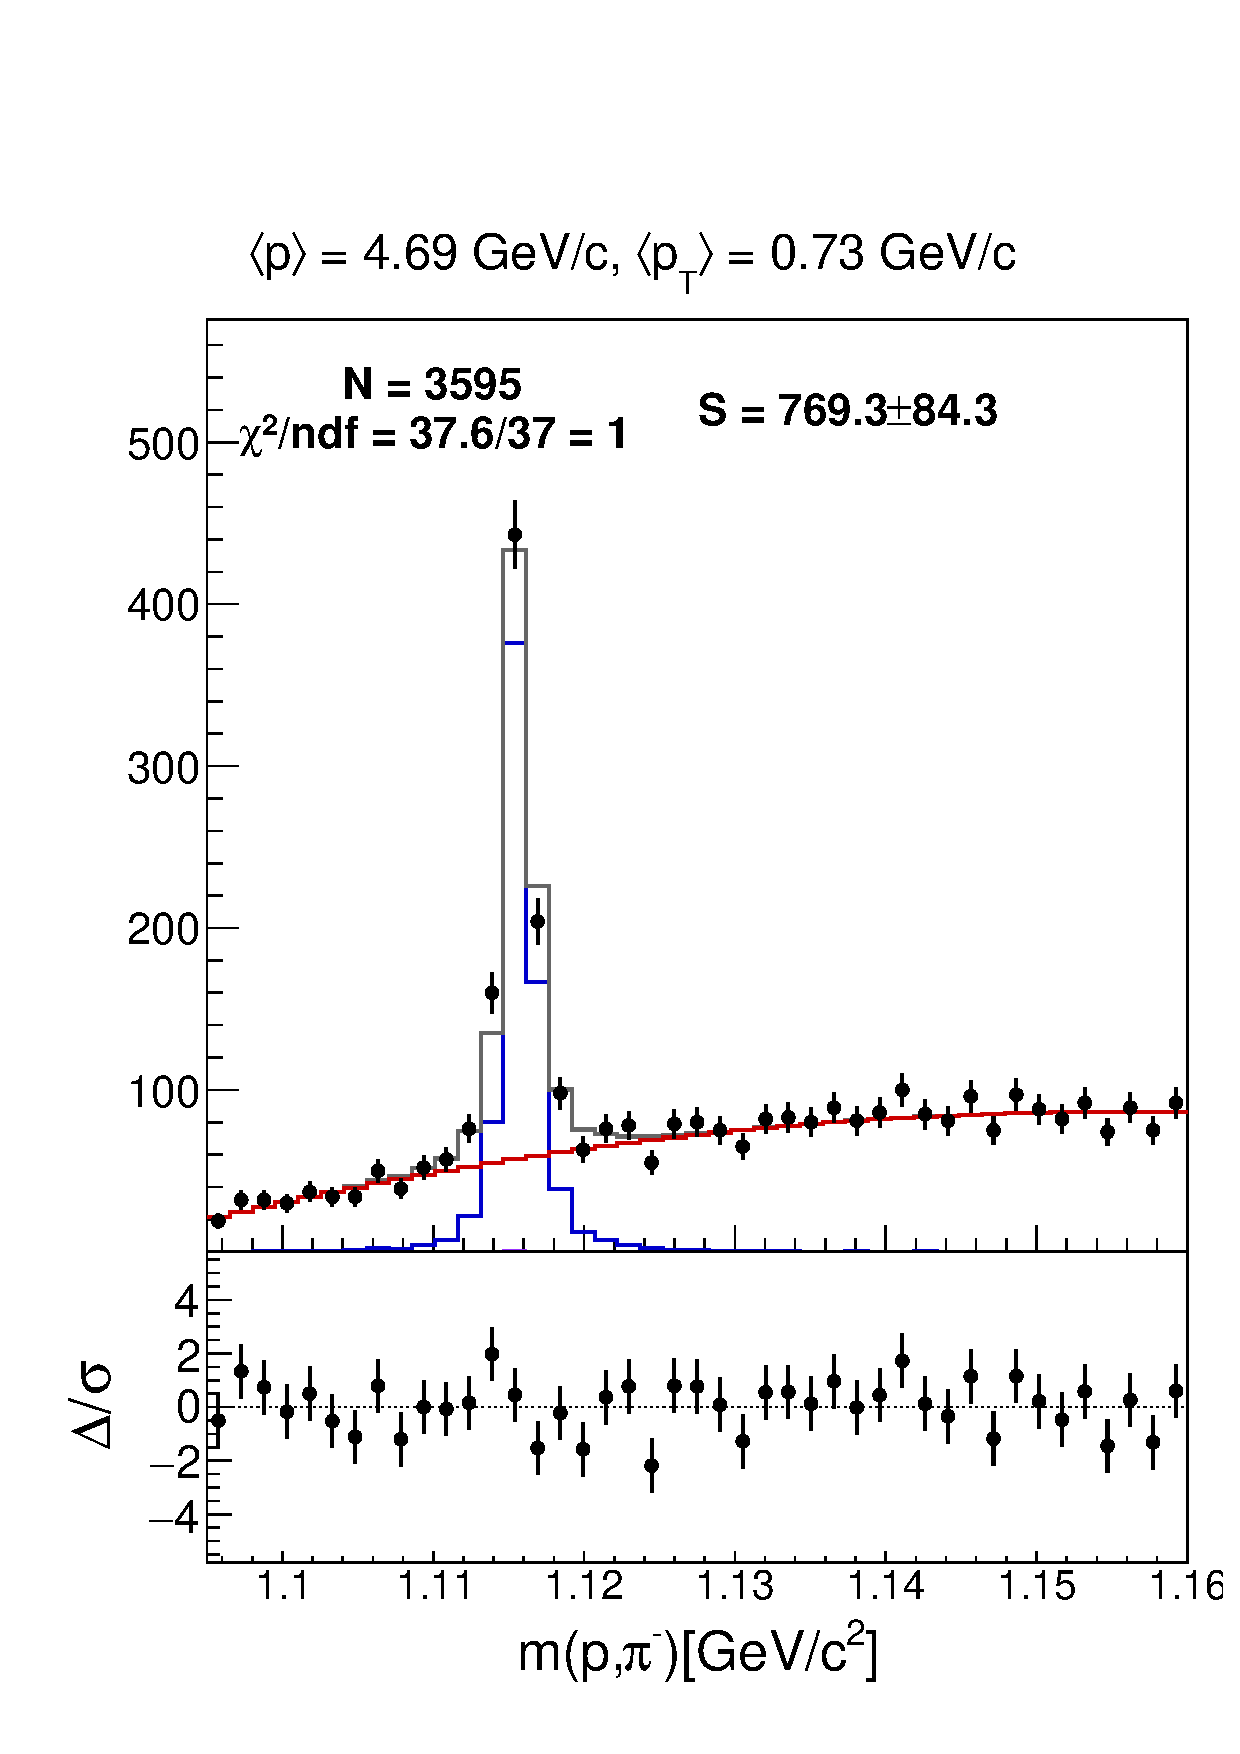
\includegraphics[clip, rviewport=0 0 1 1,width=0.32\textwidth]{vzero/mass_Data158_t0_ph1_h0_x1_y3}
  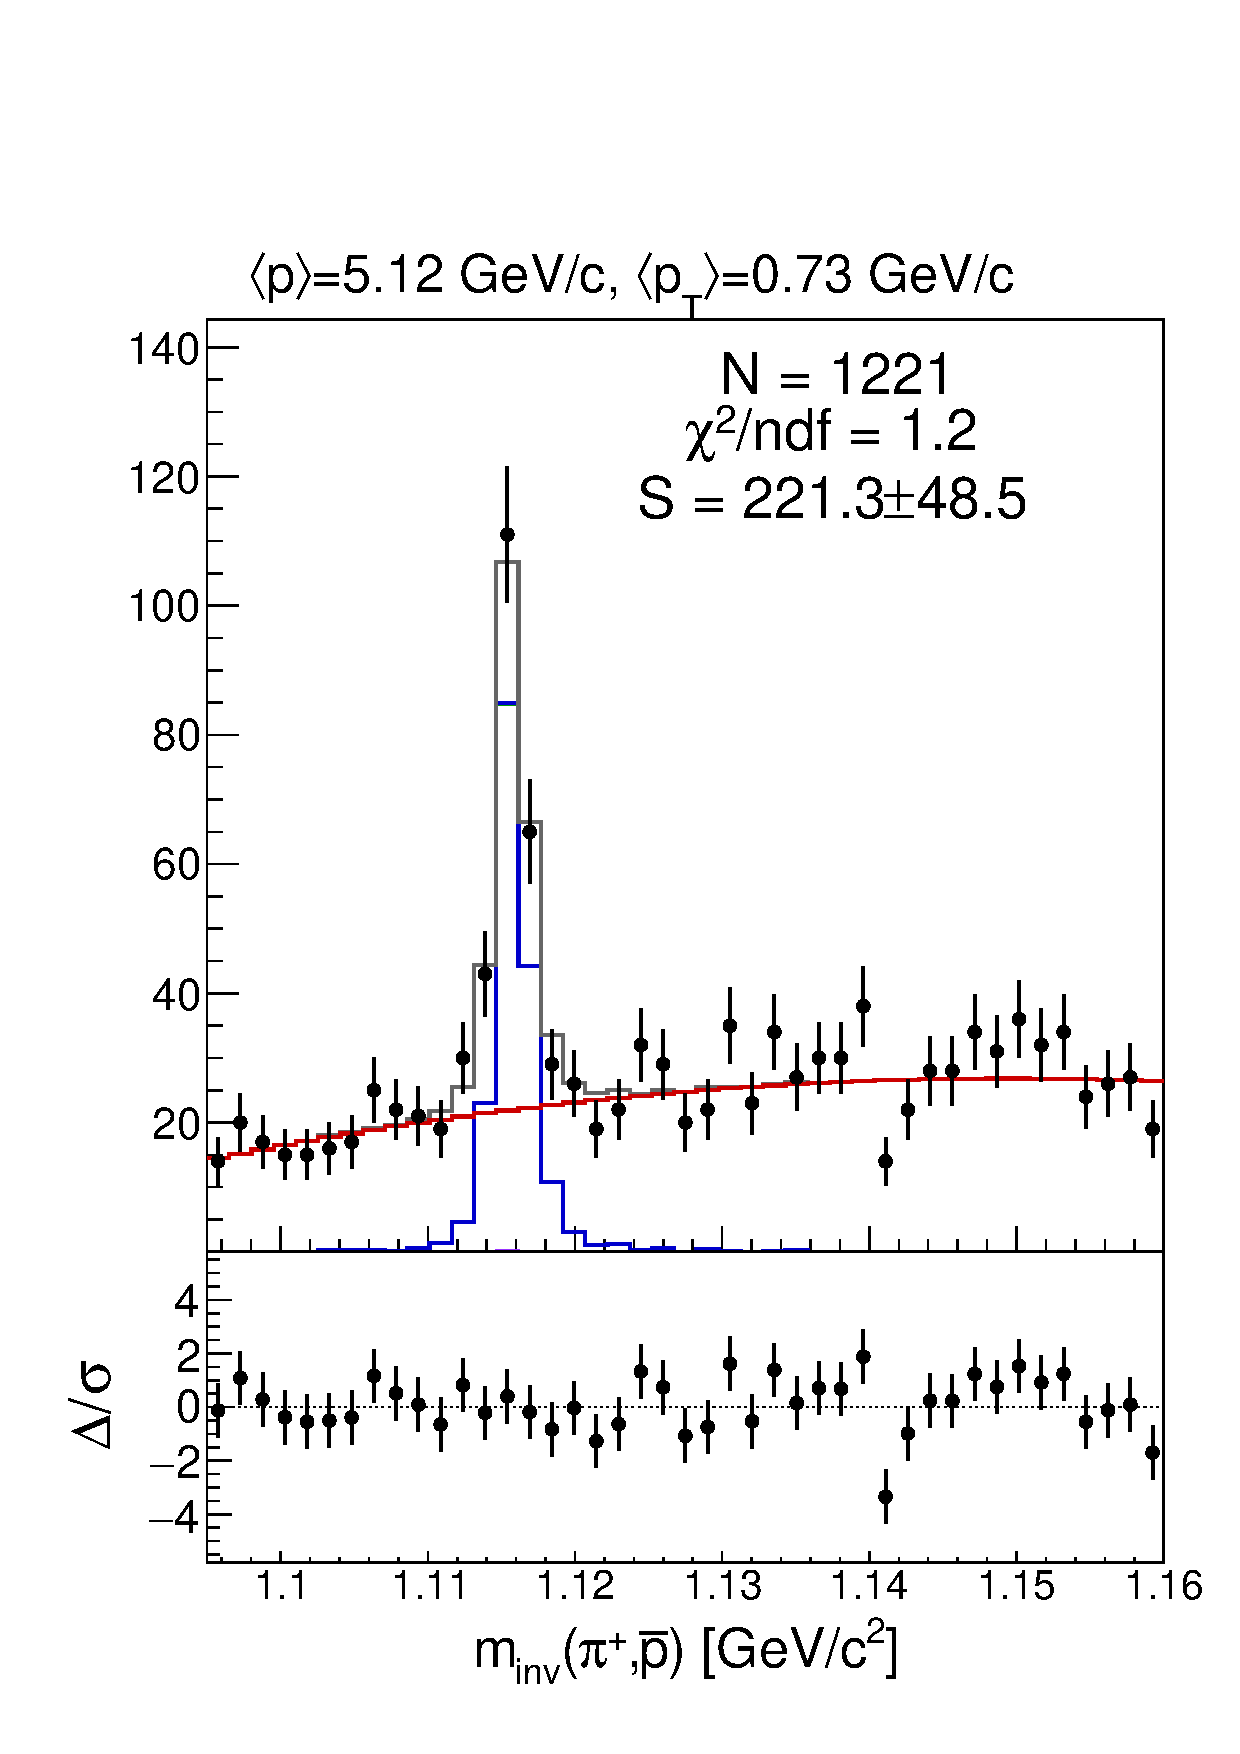
\includegraphics[clip, rviewport=0 0 1 1,width=0.32\textwidth]{vzero/mass_Data158_t0_ph1_h1_x1_y3}
  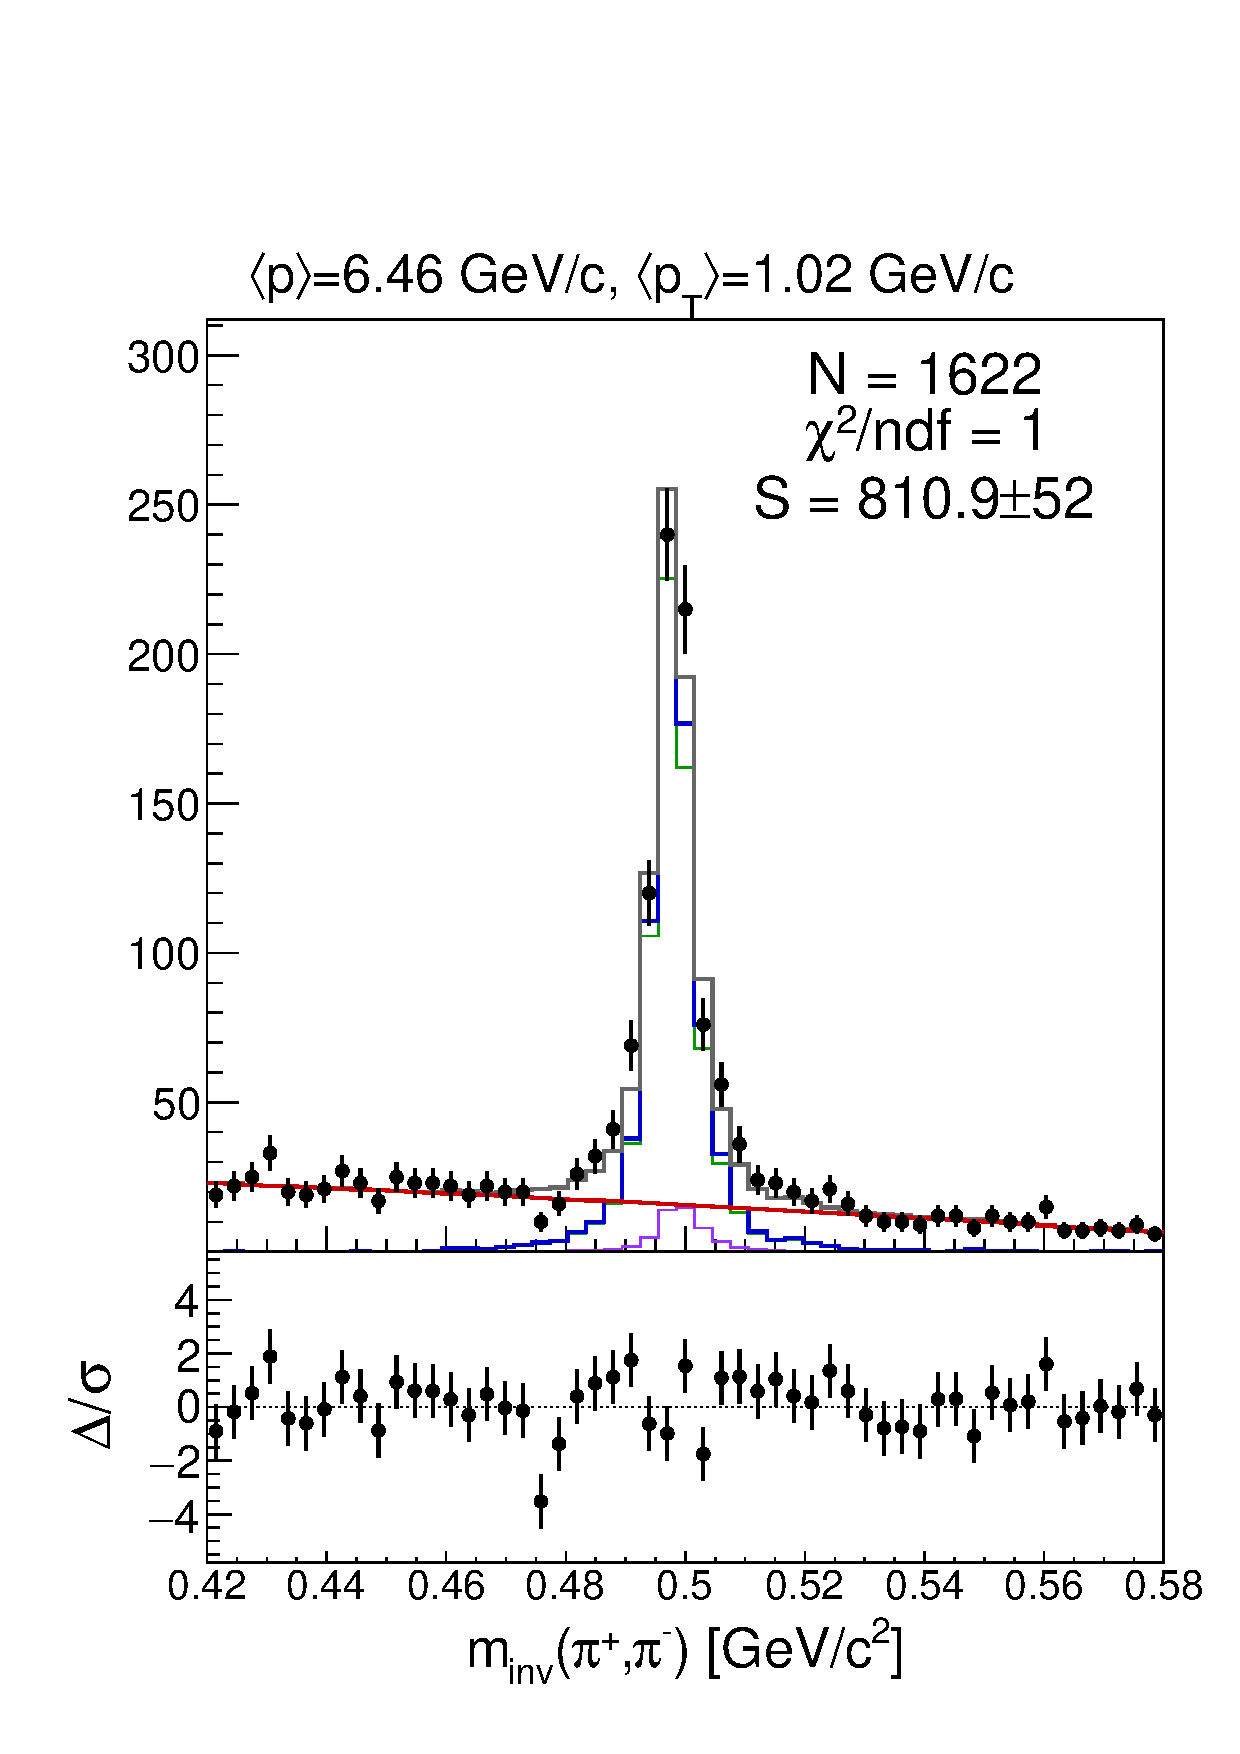
\includegraphics[clip, rviewport=0 0 1 1,width=0.32\textwidth]{vzero/mass_Data158_t0_ph1_h2_x2_y4}

  \vspace{0.5cm}
    
  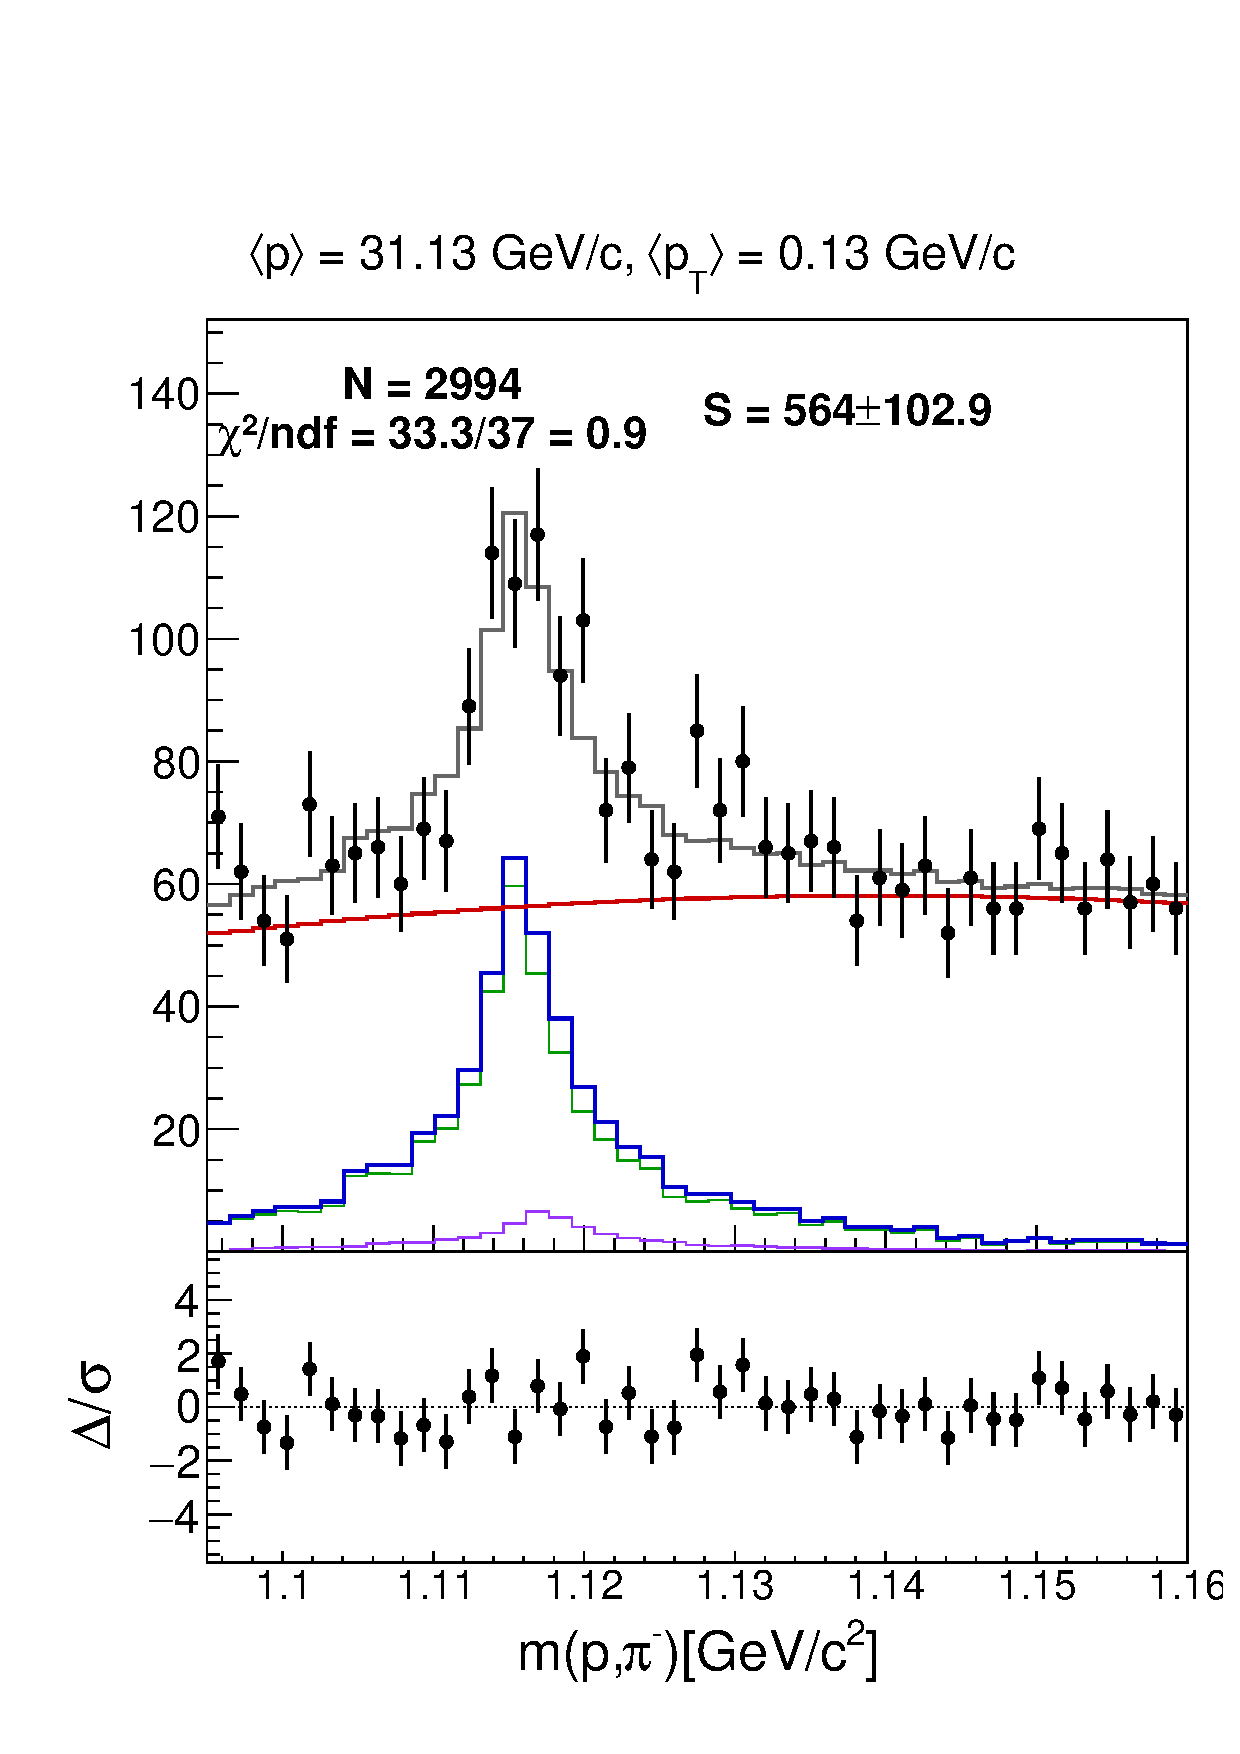
\includegraphics[clip, rviewport=0 0 1 1,width=0.32\textwidth]{vzero/mass_Data158_t0_ph1_h0_x5_y0}
  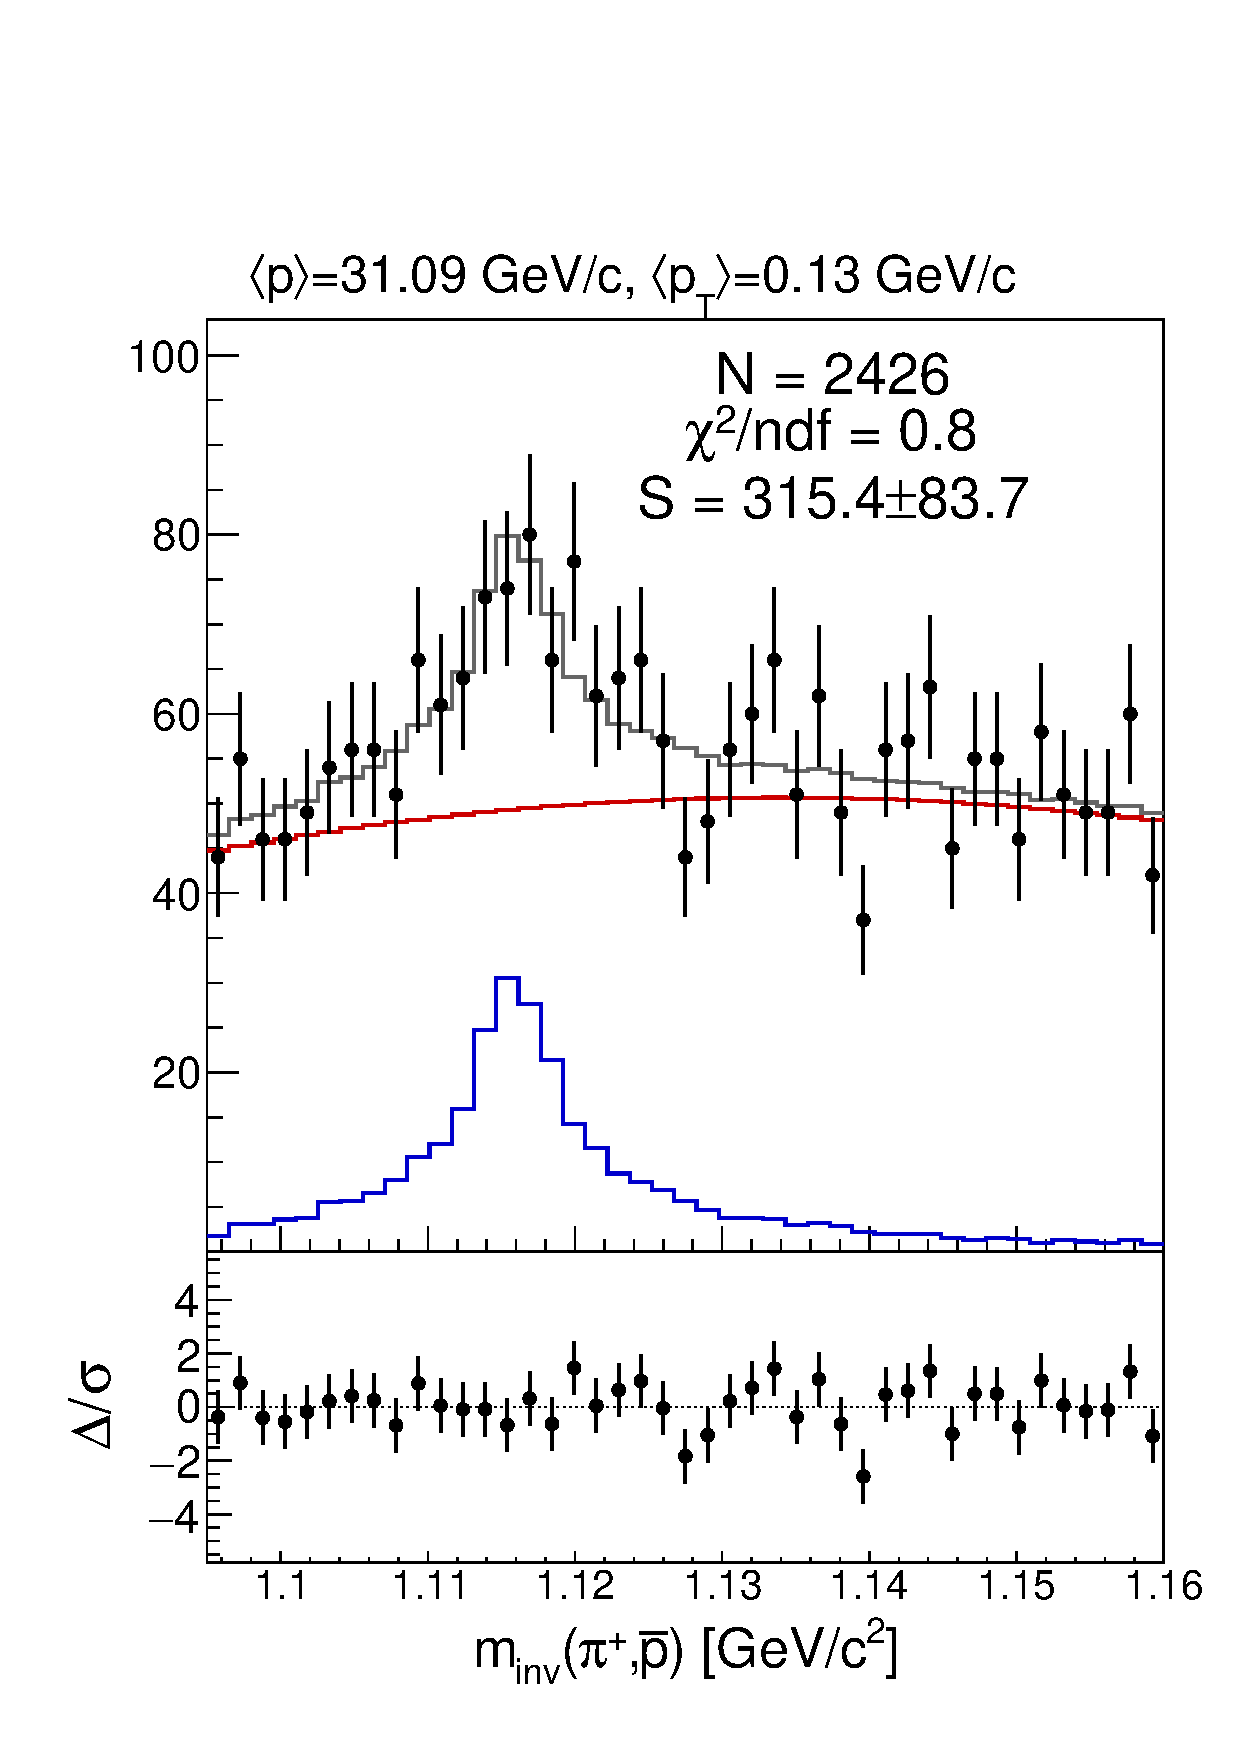
\includegraphics[clip, rviewport=0 0 1 1,width=0.32\textwidth]{vzero/mass_Data158_t0_ph1_h1_x5_y0}
  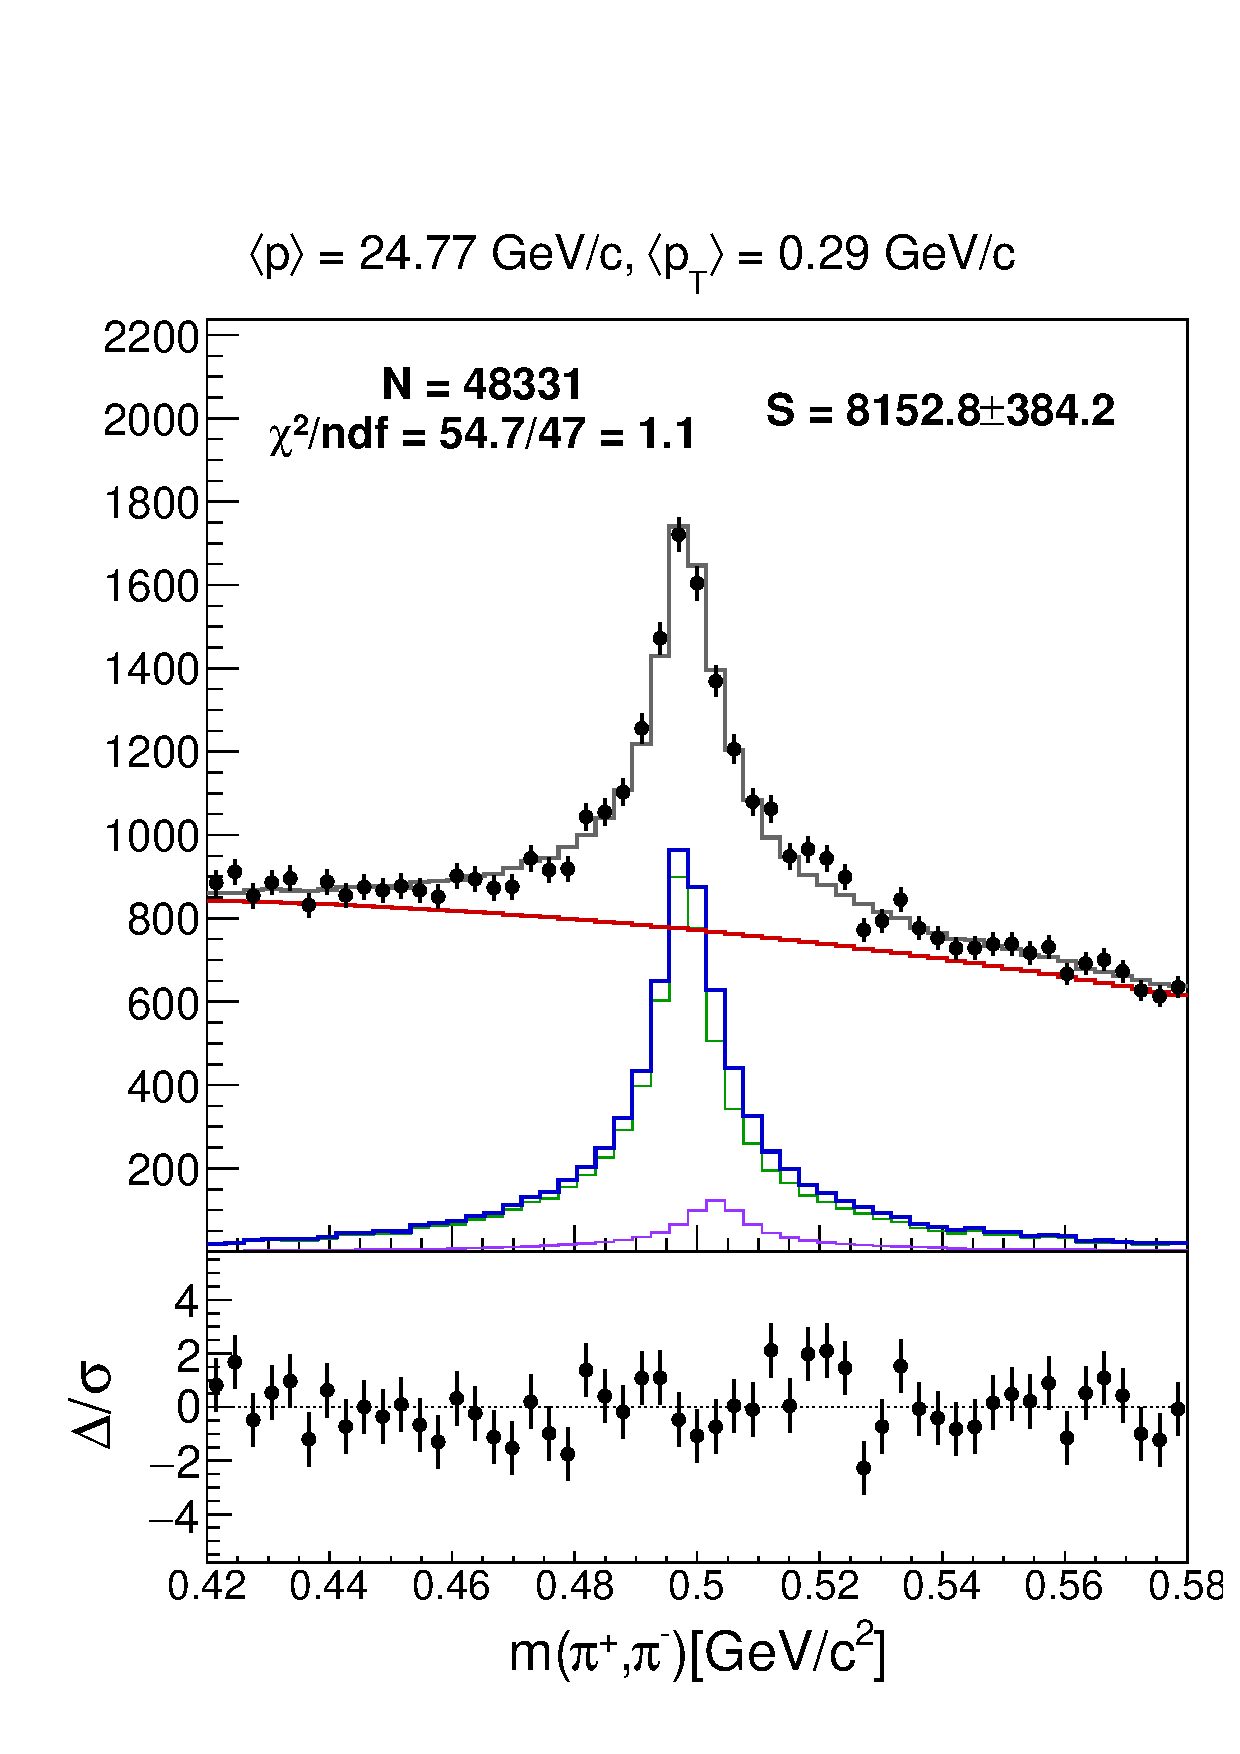
\includegraphics[clip, rviewport=0 0 1 1,width=0.32\textwidth]{vzero/mass_Data158_t0_ph1_h2_x5_y1}
  
  \caption{Examples of the fitted \minv distributions for the 158 \GeVc dataset. The plot on left, middle and right shows \lamb, \antilamb and \kzeros, respectively.}
  \label{fig:hadron:vzero:signal:dist:158:in}
\end{figure}


%%%%%%%%%%% DIST %%%%%%%%%%%%%%%%%%
\begin{figure}[!ht]
  \centering
  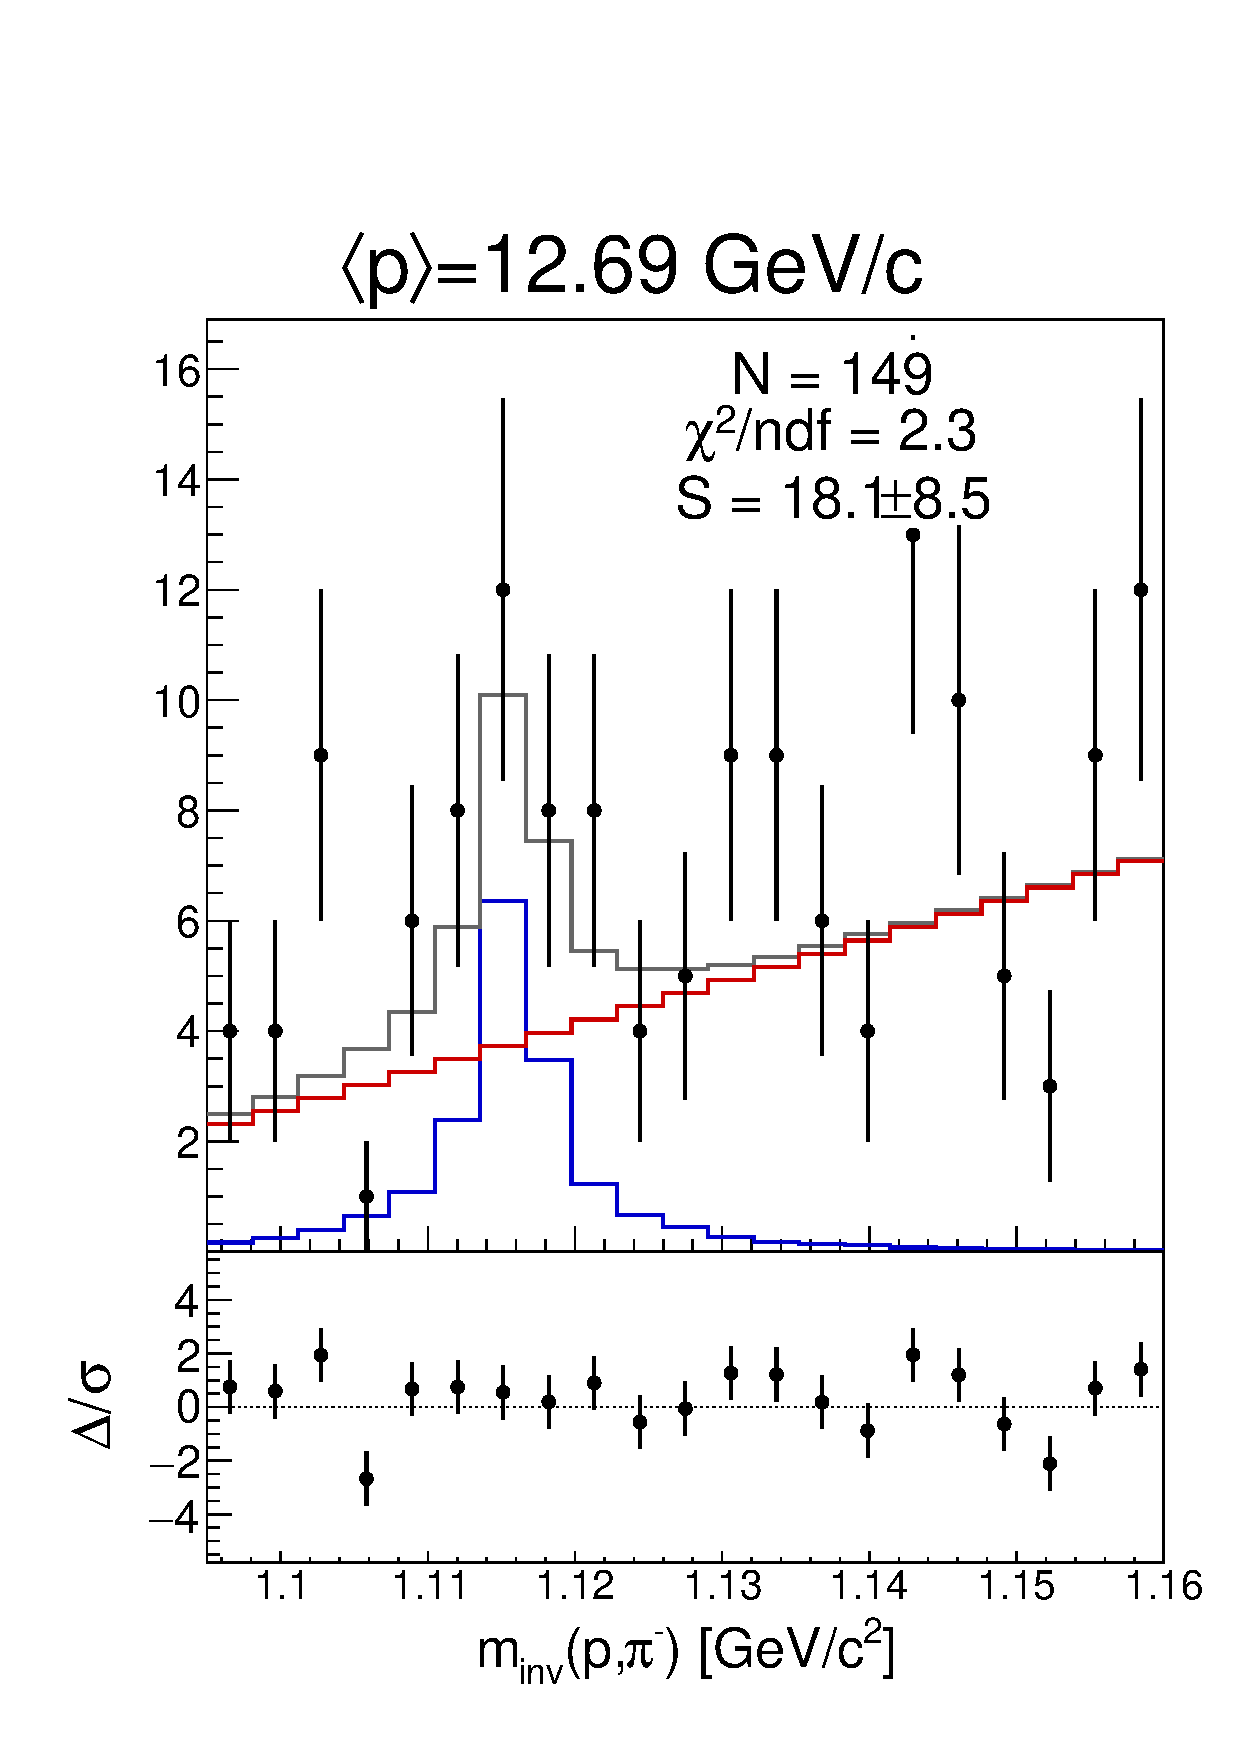
\includegraphics[clip, rviewport=0 0 1 1,width=0.32\textwidth]{vzero/mass_Data158_t1_ph0_h0_x3_y0}
  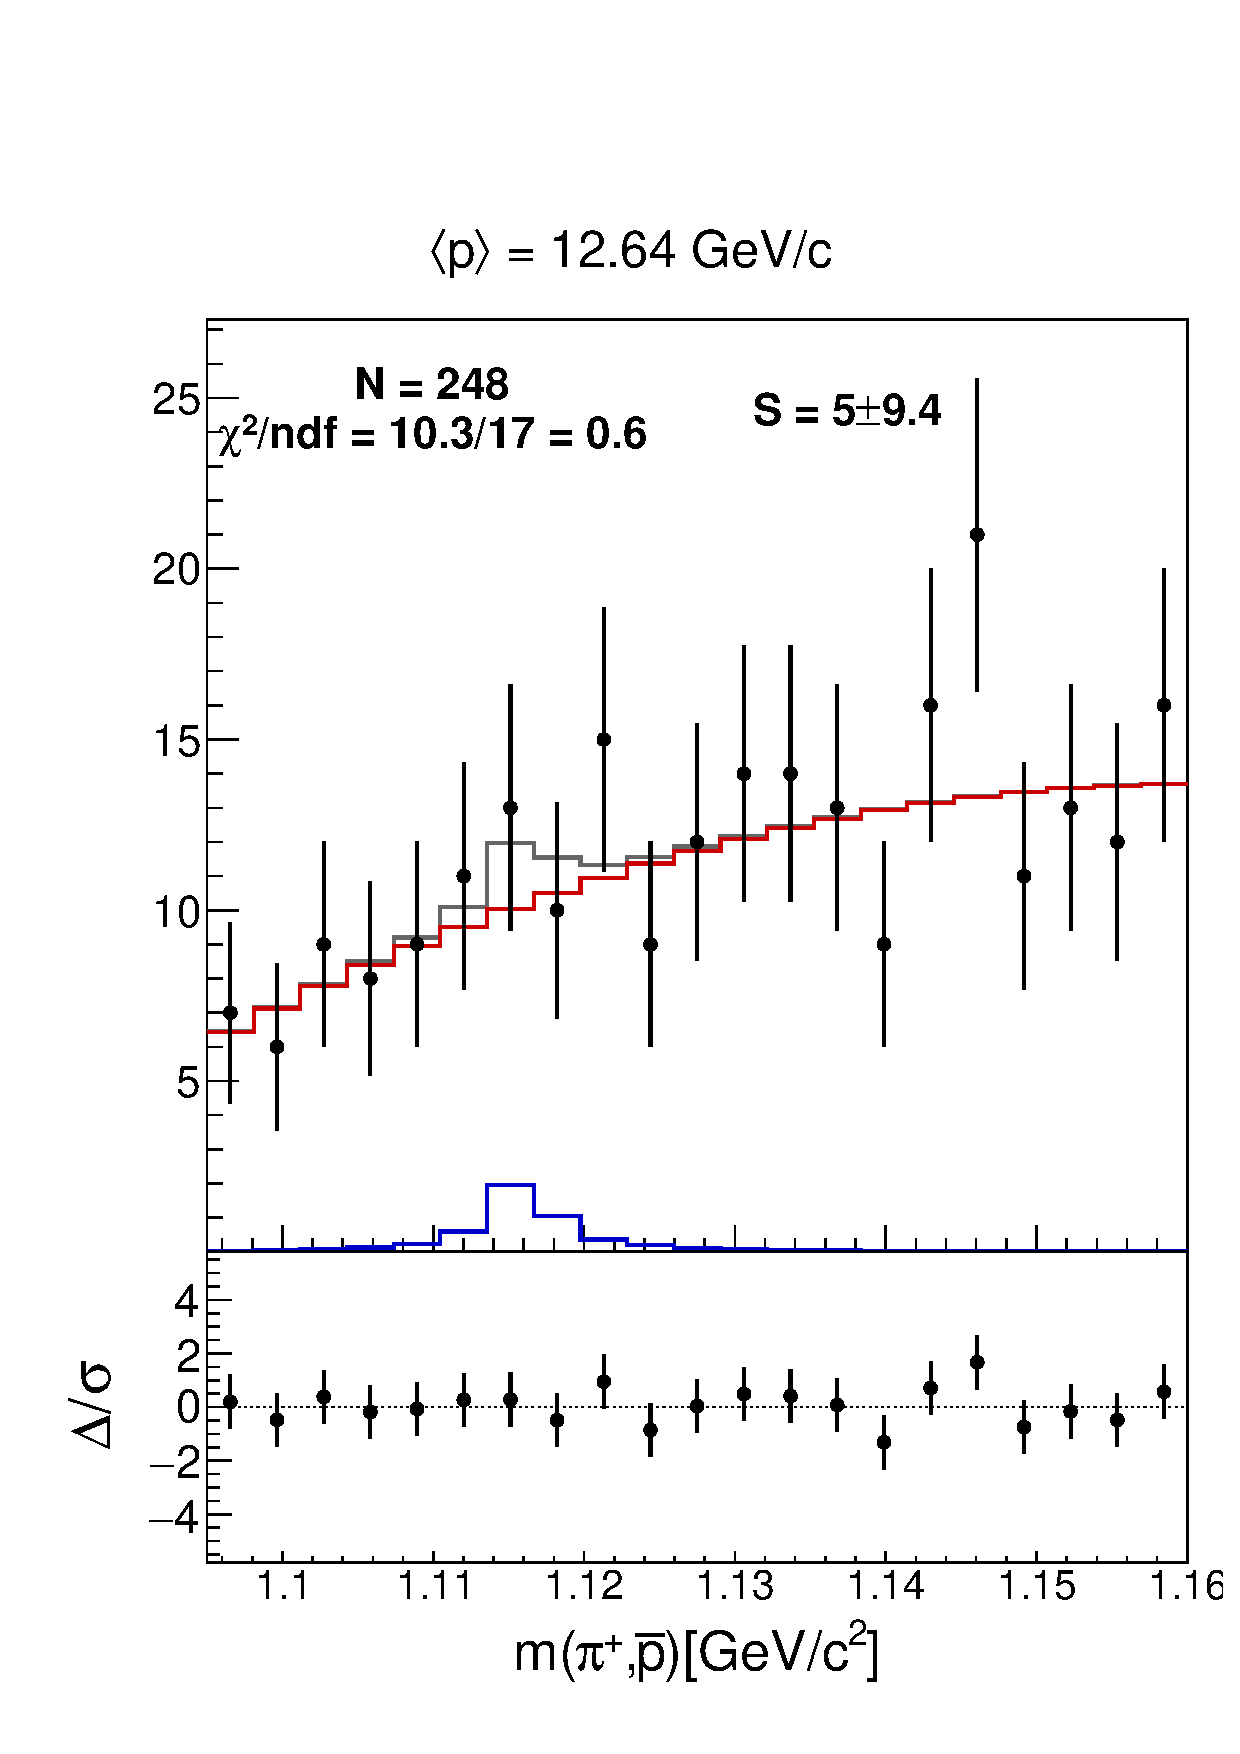
\includegraphics[clip, rviewport=0 0 1 1,width=0.32\textwidth]{vzero/mass_Data158_t1_ph0_h1_x3_y0}
  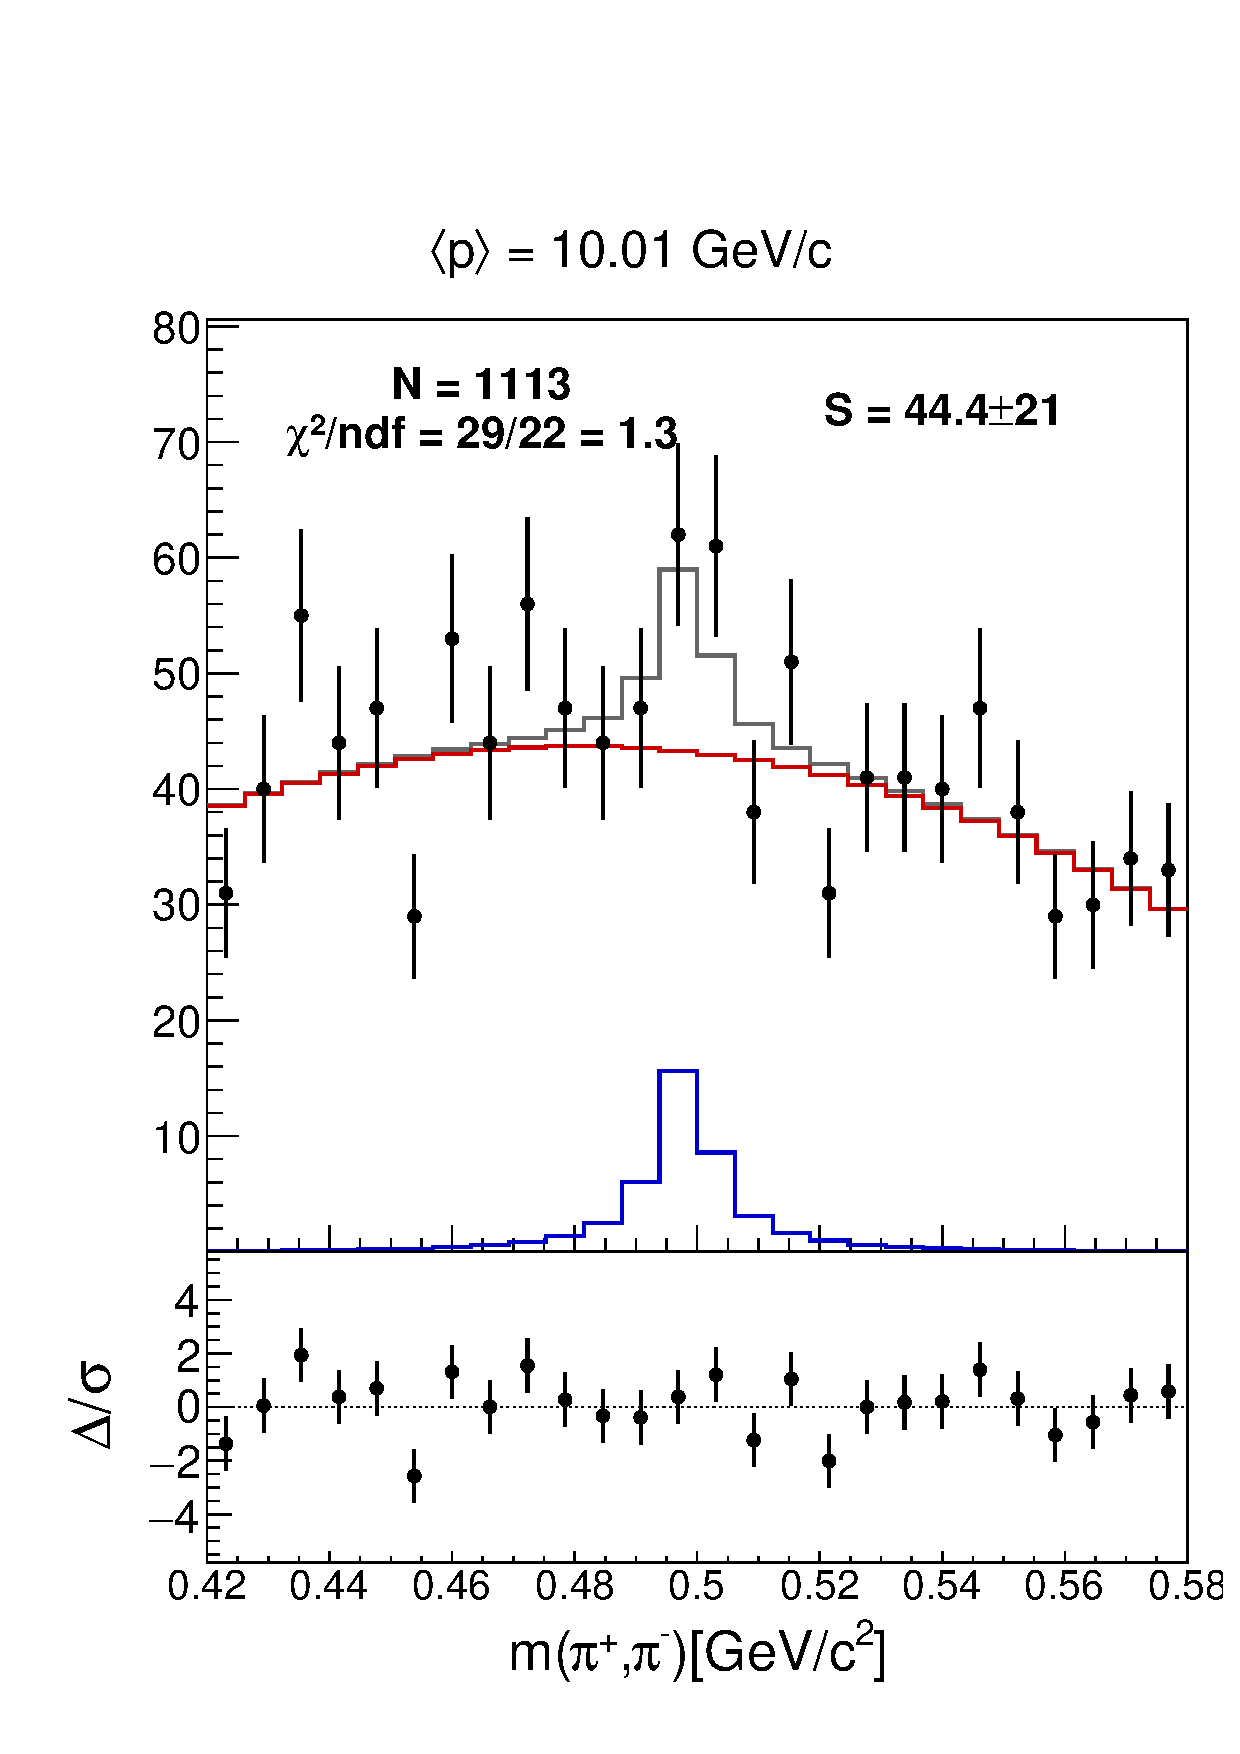
\includegraphics[clip, rviewport=0 0 1 1,width=0.32\textwidth]{vzero/mass_Data158_t1_ph0_h2_x3_y0}
  
  \caption{Examples of the fitted \minv distributions for the 158 \GeVc dataset, with target removed. The plot on left, middle and right shows \lamb, \antilamb and \kzeros, respectively.}
  \label{fig:hadron:vzero:signal:dist:158:out}
\end{figure}

%%%%%%%%%%% CHI SQ %%%%%%%%%%%%%%%%%%
\begin{figure}
  \centering
  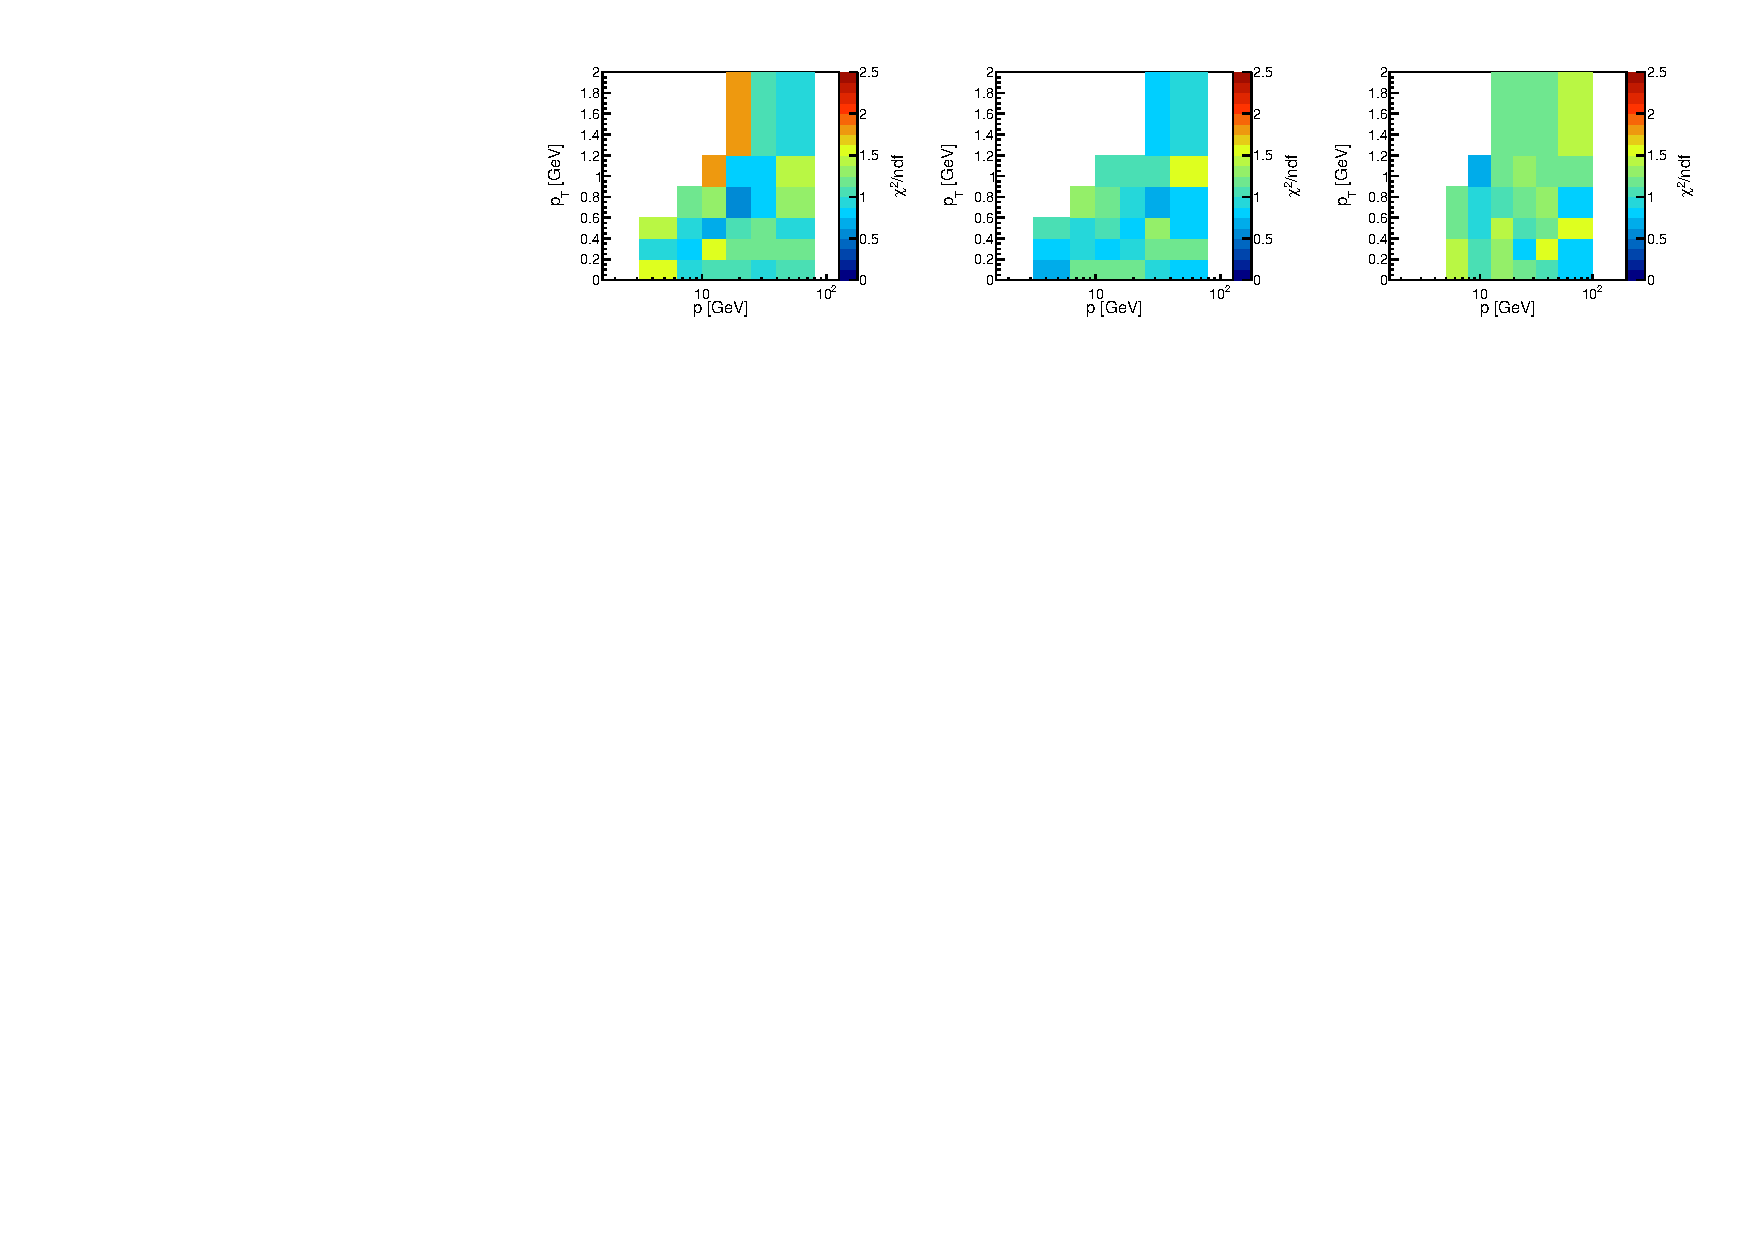
\includegraphics[clip, rviewport=0 0 1 1,width=0.99\textwidth]{vzero/chisq_Data158_t0_ph1}
  
  \caption{}
  \label{fig:hadron:vzero:signal:chi:158}
\end{figure}


The reduced $\chi^2$ of the \minv fit of the target inserted datasets are shown
in~\cref{fig:hadron:vzero:signal:chi:158,fig:hadron:vzero:signal:chi:350}.
Since the values of $\chi^2/ndf$ are in all phase space bins around 1
and very few bins show $\chi^2/ndf \sim 1.5$, we can conclude that the
measured \minv fit is well described by our \minv model.   
The extracted signal $S$ for the target inserted and removed datasets are shown
in~\cref{fig:hadron:vzero:signal:extracted:158in,fig:hadron:vzero:signal:extracted:350in,fig:hadron:vzero:signal:extracted:158out,fig:hadron:vzero:signal:extracted:350out}.


%%%%%%%%%%% EXTRACTED SIGNAL %%%%%%%%%%%%%%%%%%
\begin{figure}
  \centering
  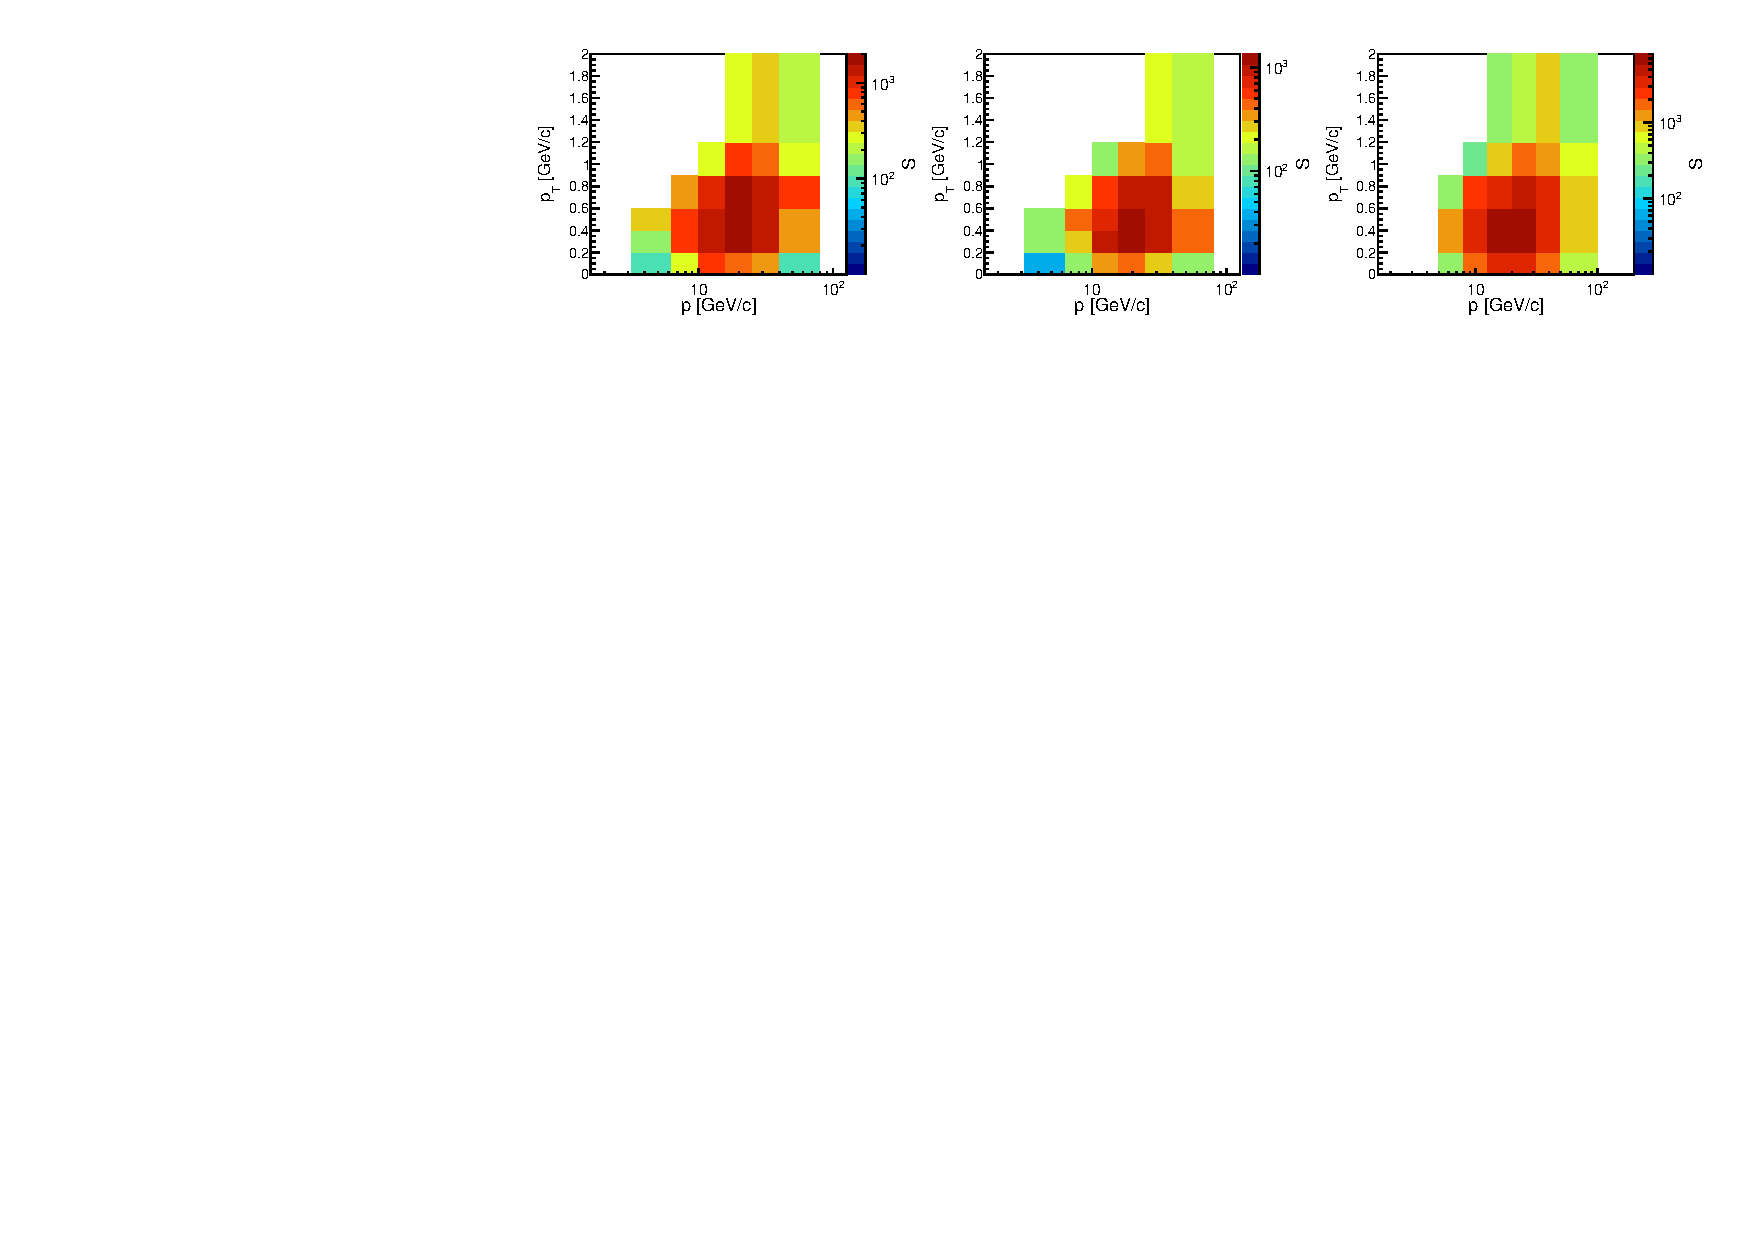
\includegraphics[clip, rviewport=0 0 1 1,width=0.99\textwidth]{vzero/signal_Data158_t0}
  
  \caption{}
  \label{fig:hadron:vzero:signal:extracted:158in}
\end{figure}

%%%%%%%%%%% EXTRACTED SIGNAL %%%%%%%%%%%%%%%%%%
\begin{figure}
  \centering
  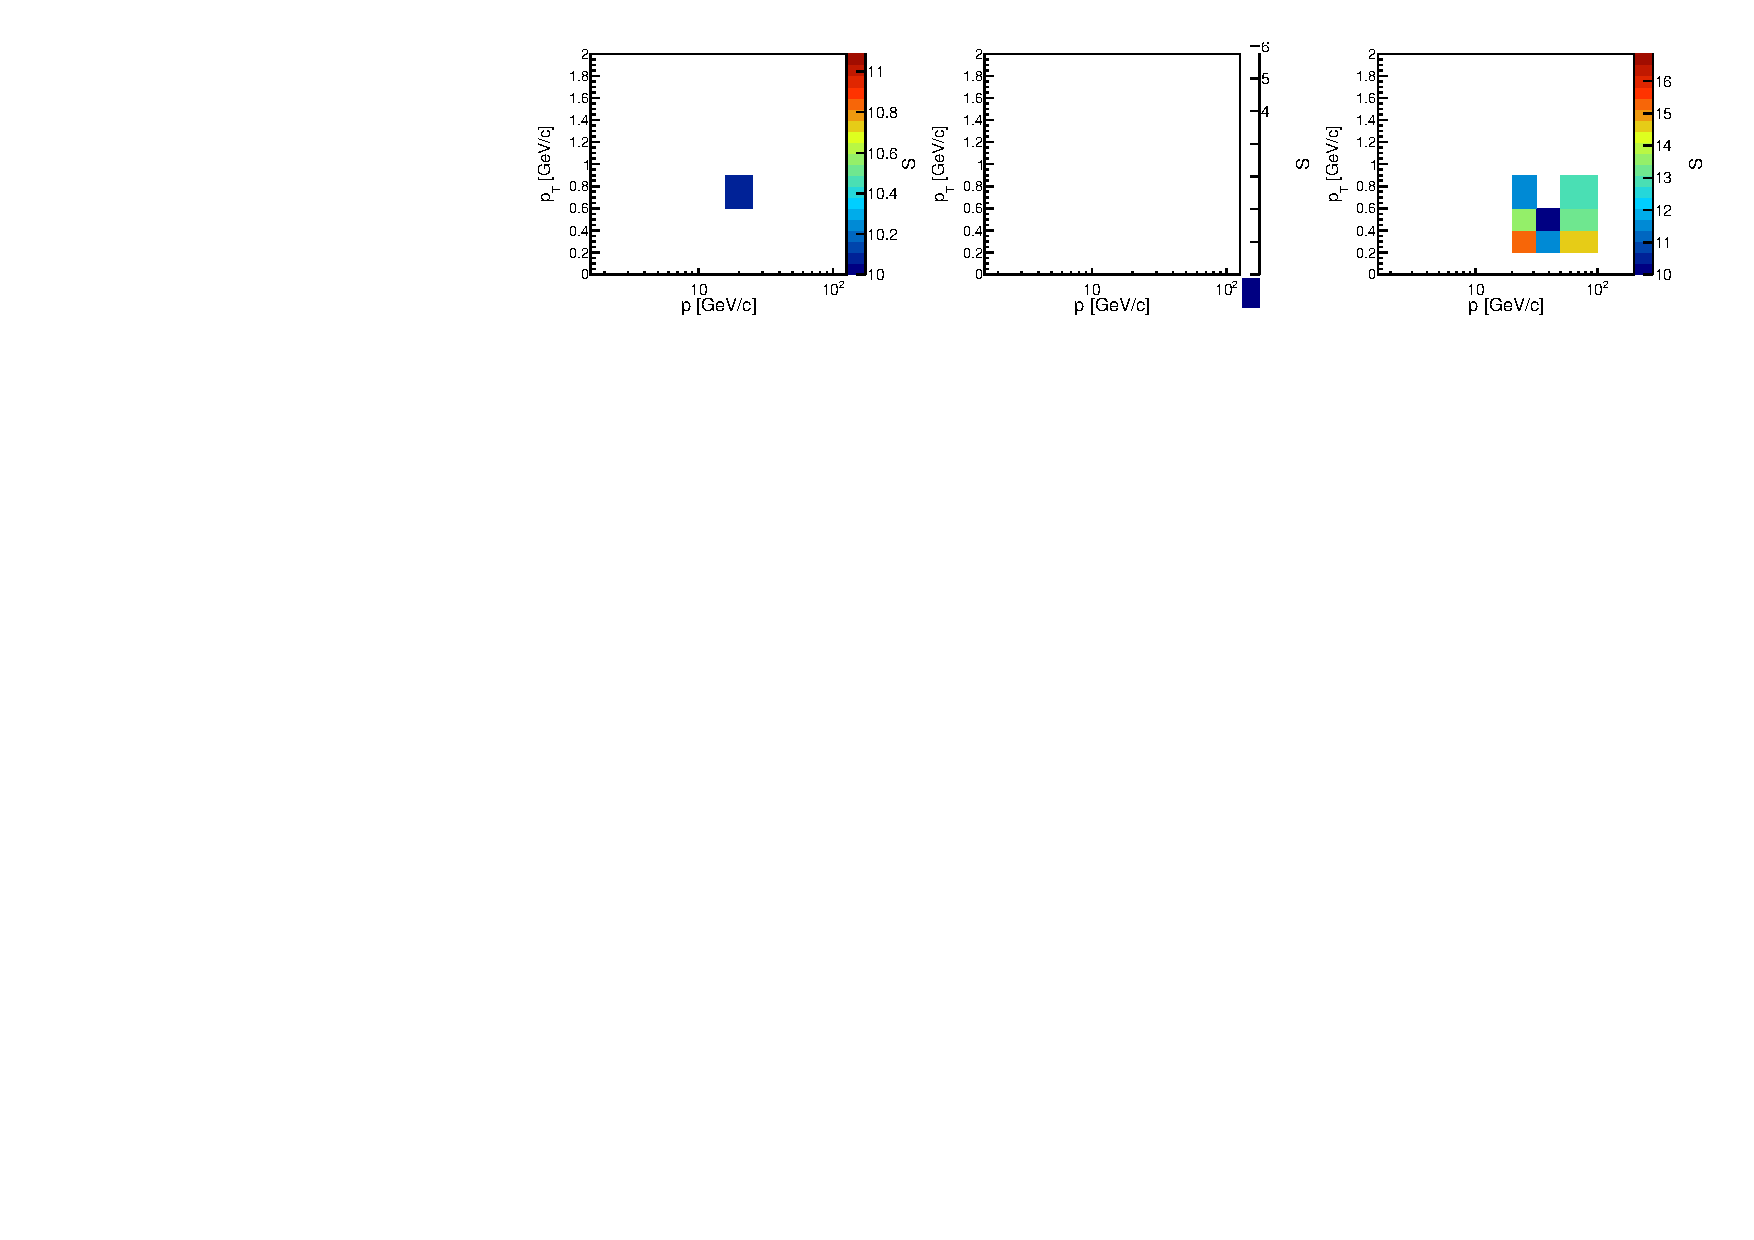
\includegraphics[clip, rviewport=0 0 1 1,width=0.99\textwidth]{vzero/signal_Data158_t1}
  
  \caption{}
  \label{fig:hadron:vzero:signal:extracted:158out}
\end{figure}



%%%%%%%%%%%%%%%%%%%%%%%%%%%%%%%%%%%%%%%%
\section{Monte Carlo corrections}
\label{sec:hadron:correction}

\note{TO REVIEW}

The measured number of events, tracks and \vzeros
particles in a given phase space bin are naturally biased by
detector effects. To determine the final spectra,
these effects must be corrected, and that
is done by applying a correction factor obtained
from Monte Carlo simulations. This factor is called here \cmc.
For a given phase space bin, \cmc is basically the ratio
between the generated and measured spectra and it
is written as
\begin{equation}
  \cmc = \left( \frac{n^\gen}{N^\gen} \right) / \left( \frac{n^\sel}{N^\sel} \right).
  \label{eq:hadron:correction:cmc}
\end{equation}
where $N$ refers to number of events and $n$ can be either the number of
tracks, for the identified spectra analysis, or the number
of \vzeros, for the \vzero analysis.
The indexes \gen and \sel refer to generated and selected quantities and,
while the first is obtained directly from the Monte Carlo generators,
the second is obtained by the detector simulations, in which the
reconstruction algorithm and selection are exactly the same
as the one applied to data.
For the sake of clearness, the \cmc can be split in the
event and track or \vzero contributions, which will be refereed as
$\alpha$ and $\beta$. In this way, \cmc becomes
\begin{equation}
  \cmc = \left( \frac{N^\sel}{N^\gen} \right) / \left( \frac{n^\sel}{n^\gen} \right) = \alpha / \beta.
  \label{eq:hadron:correction:cmc:2}
\end{equation}
The $\alpha$ factor is common to all the datasets,
while the $\beta$ is different for each phase space bin. 

The \cmc was determined here by 
the three simulation sets, generated with different hadronic
interaction models (see~\cref{sec:hadron:data}).
The $\alpha$ factor obtained is summarized
in~\cref{tab:hadron:alpha}, where we show the values for each simulation
set and their average value, which will be used in this work. 
The observed differences in the $\alpha$ factor due
to the hadronic interaction models are expected mainly
because of the large discrepancy between the particle
multiplicities. As an illustration, we can take the \DPMJetLong
case, in which the average multiplicity is
fairly larger than the others and consequently the
$\alpha$ is also significantly larger. 
This relation is caused mainly by two effects. First,
the interaction trigger probability is larger on average
because the larger number of particles crossing the detector.
Second, the cut on the Z position of the main vertex
tends to remove less events since, with more detected particles,
the fit of main vertex tends to be more precise.
The model dependence of the $\alpha$ will be accounted
on the systematic uncertainties in~\cref{sec:hadron:spec:syst}.

\begin{table}
  \begin{center}
    \begin{tabular}{|r|c|c|} \hline
      & 158 GeV/c & 350 GeV/c \\ \hline
      \EposLong   & 0.875     & 0.744 \\
      \DPMJetLong & 0.949     & 0.848 \\
      \QGSJetLong & 0.868     & 0.721 \\ \hline
      Average     & 0.897     & 0.771 \\ \hline
    \end{tabular}
    \caption{}
    \label{tab:hadron:alpha}
  \end{center}
\end{table}

The $\beta$ factor for \pions, \kaons and \protons
is computed by the ratio of the generated and
measured number of tracks. 
In~\cref{fig:hadron:correction:beta:dedx158,fig:hadron:correction:beta:dedx350}
we show the $\beta$ for these particles.
For the \vzero particles, \lambs and \kzeros, the $\beta$
is computed as the ratio between the \vzero particles generated and
measured in a given phase space bin.
In~\cref{fig:hadron:correction:beta:vzero158,fig:hadron:correction:beta:vzero350}
we show the $\beta$ for these particles.
It is important to note that the $\beta$ factor
for the \vzero particle includes the effect
of the \vzero cuts, presented in~\cref{sec:hadron:signal:cuts}.


%%%%%%%%%% BETA %%%%%%%%%%%%%%%%
\begin{figure}
  \centering
  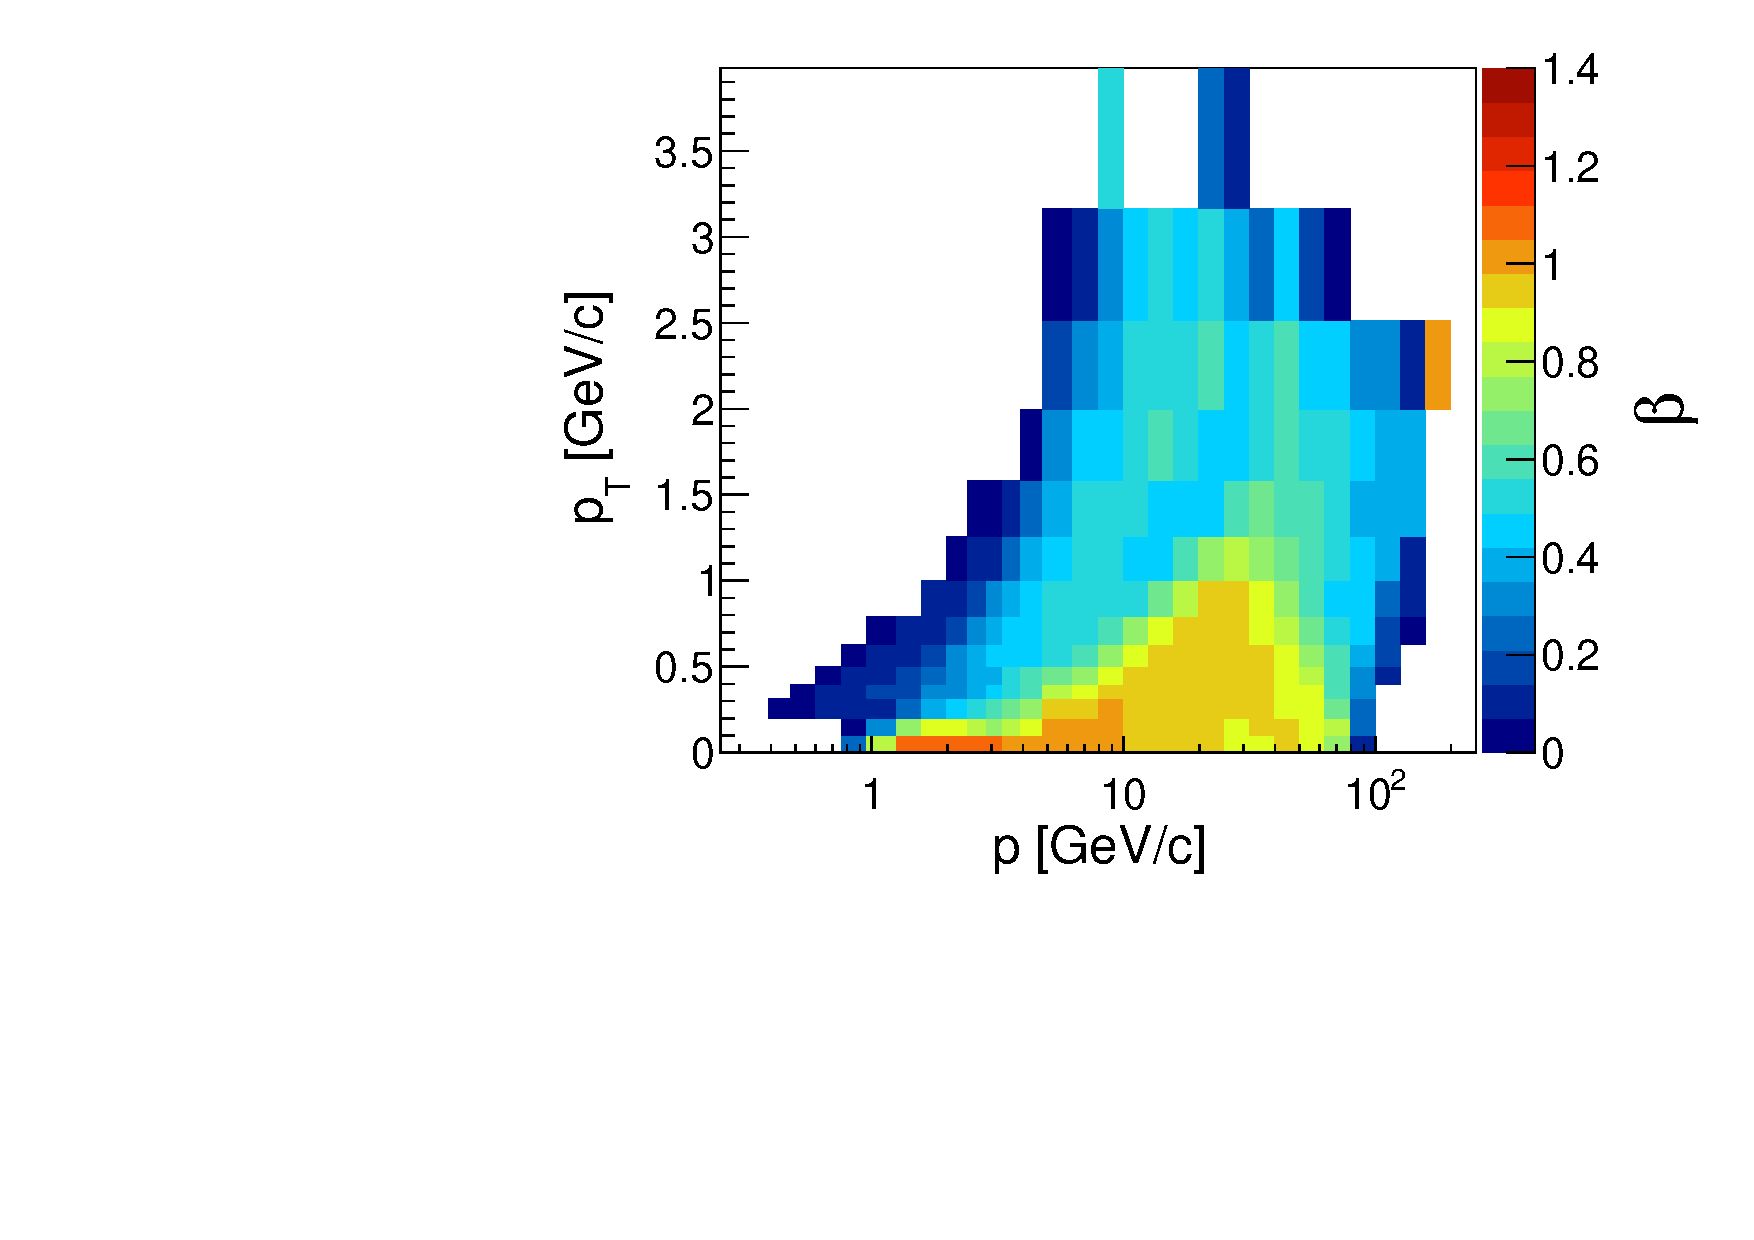
\includegraphics[clip, rviewport=0 0.13 1 0.94,width=0.4\textwidth]{dedx/fac_158_All_beta_c0_p1}
  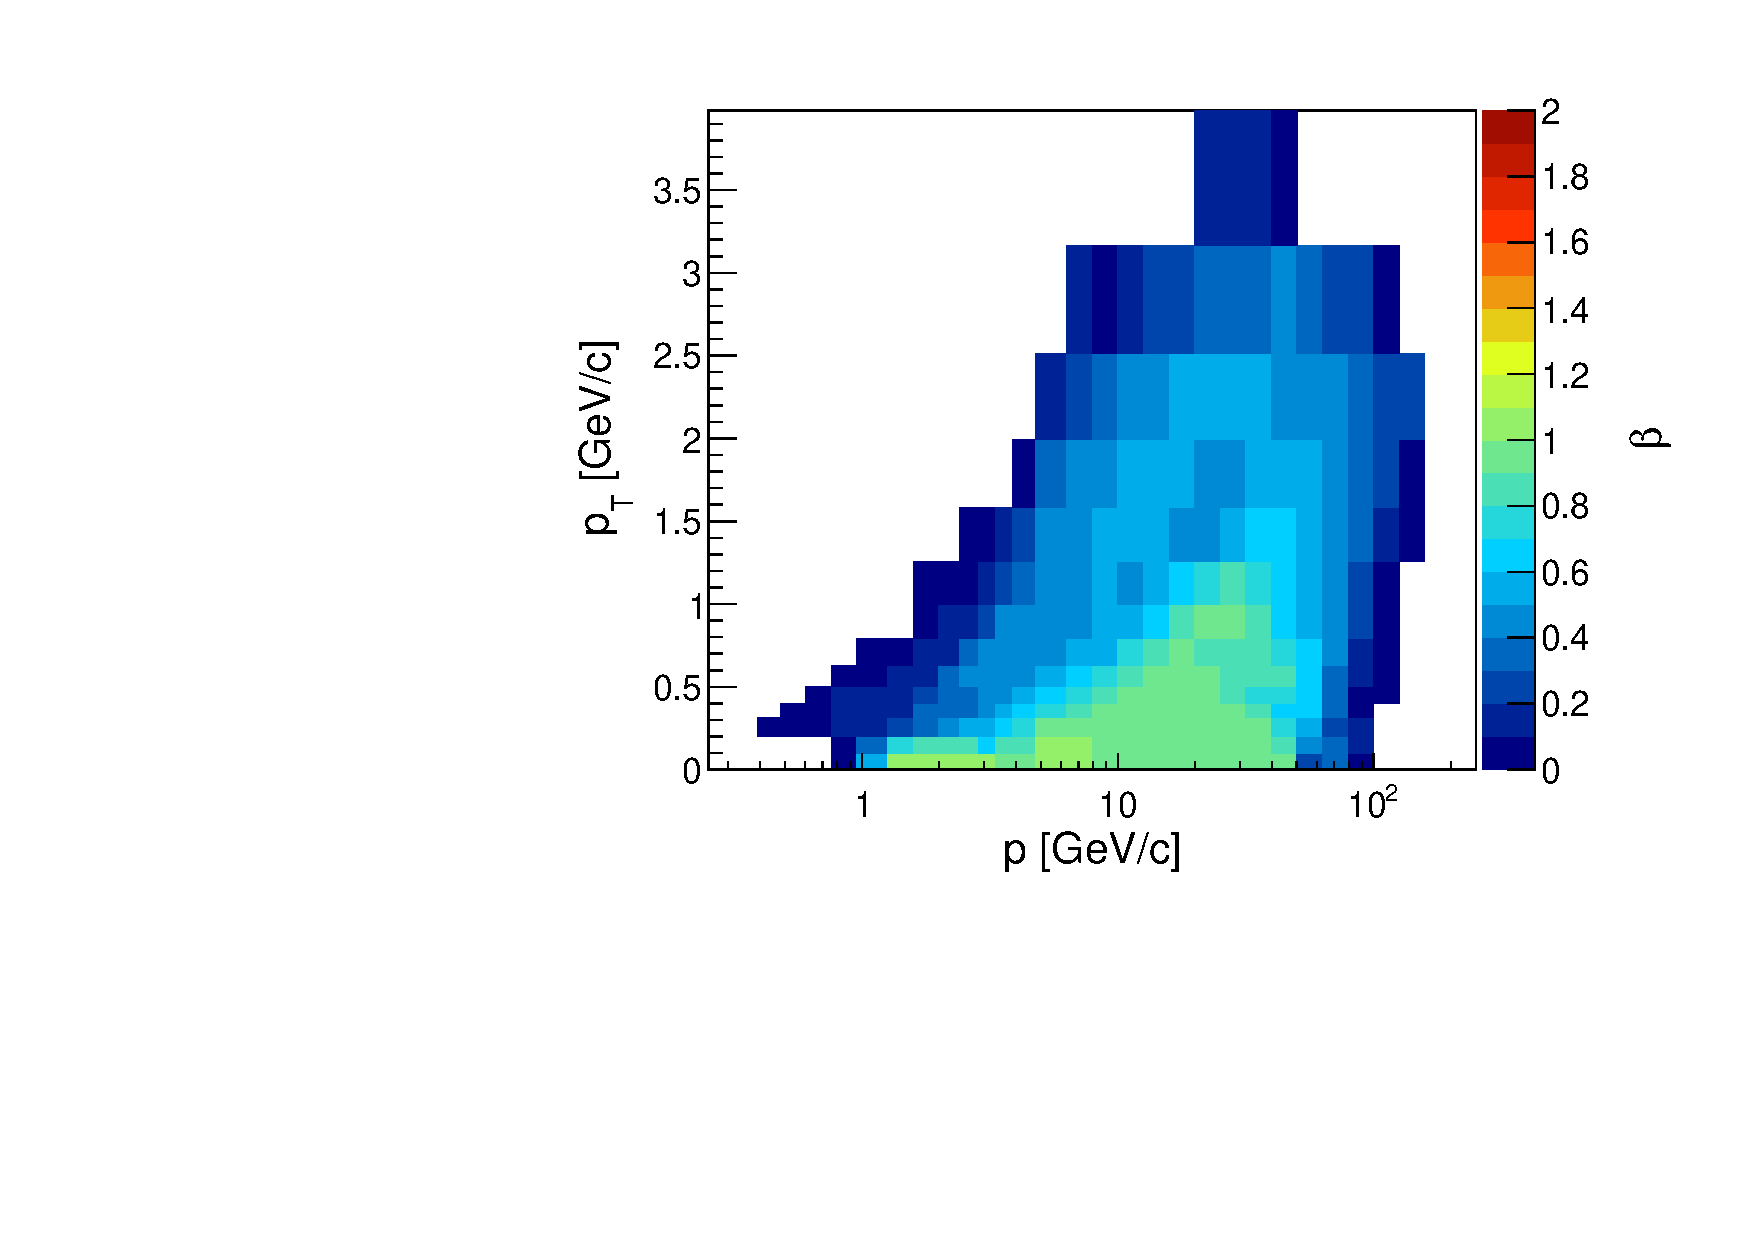
\includegraphics[clip, rviewport=0 0.13 1 0.94,width=0.4\textwidth]{dedx/fac_158_All_beta_c1_p1}

  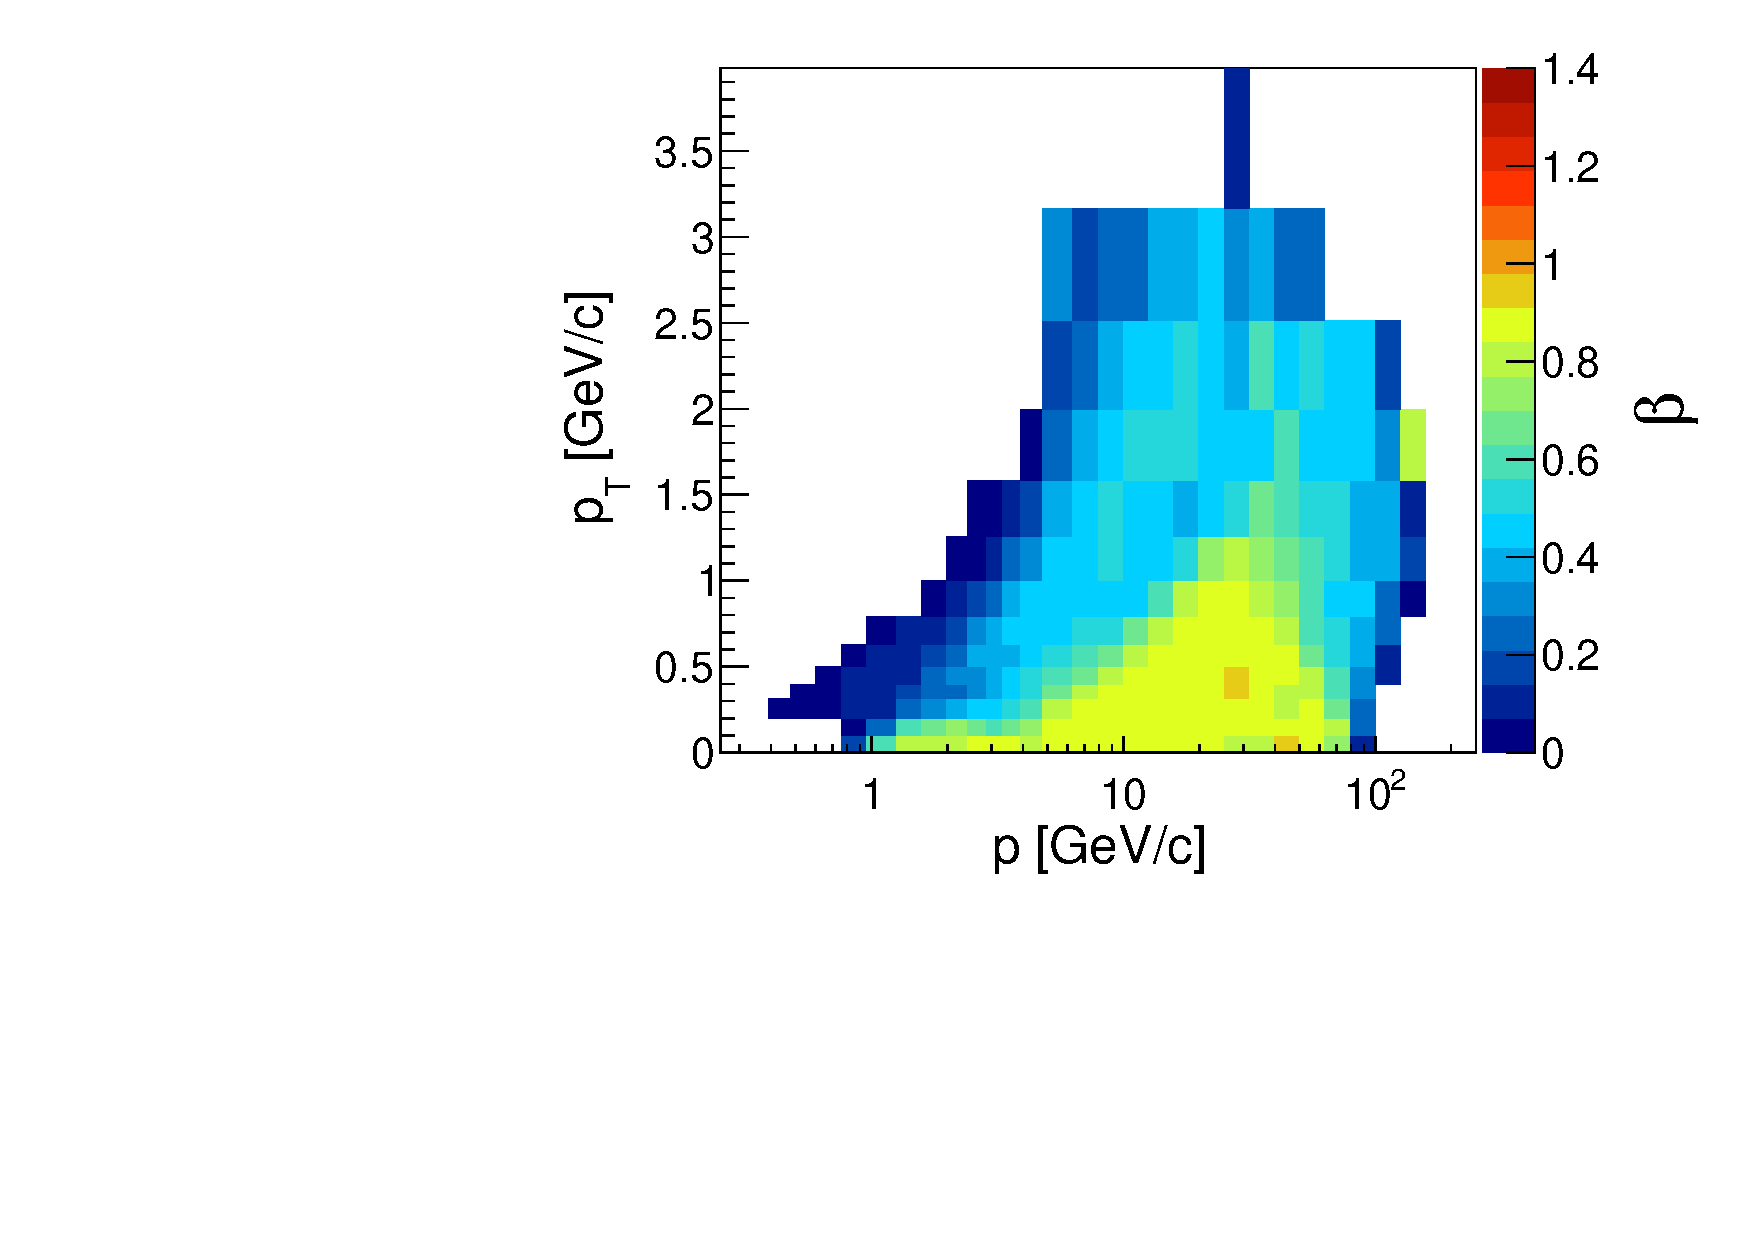
\includegraphics[clip, rviewport=0 0.13 1 0.94,width=0.4\textwidth]{dedx/fac_158_All_beta_c0_p2}
  \includegraphics[clip, rviewport=0 0.13 1 0.94,width=0.4\textwidth]{dedx/fac_158_All_beta_c1_p2}

  \includegraphics[clip, rviewport=0 0.13 1 0.94,width=0.4\textwidth]{dedx/fac_158_All_beta_c0_p3}
  \includegraphics[clip, rviewport=0 0.13 1 0.94,width=0.4\textwidth]{dedx/fac_158_All_beta_c1_p3}

  \caption{$\beta$ correction factor for the 158 \GeVc dataset.}
  \label{fig:hadron:correction:beta:dedx158}
\end{figure}

%%%%%%%%%%% BETA %%%%%%%%%%%%%%%%%%
\begin{figure}
  \centering
  \includegraphics[clip, rviewport=0 0 1 1,width=0.95\textwidth]{vzero/beta158}
  
  \caption{$\beta$ correction factor for the 158 \GeVc dataset.}
  \label{fig:hadron:correction:beta:vzero158}
\end{figure}

The geometrical acceptance of the detector
is the dominant contribution to the $\beta$ factor
for both charged hadrons and \vzero particles.
Smaller effects, but still significant, are related
to the event selection, track and \vzero reconstruction efficiency, 
bin migration and feed-down from re-interactions and weak decays.
The model dependence of the $\beta$ factor is only significant (> 1\%) for the
contributions of the event selection and feed-down from weak decays.
The latter case will be approached in~\cref{sec:hadron:correction:fd}.
For the event selection, the differences between the three models
can reach up 10\% for some phase space bins, in which the contribution
of both the T2 selection and the cut on the main vertex Z position are accounted for.
The differences will be taken into account on the systematic uncertainties
of the spectra (see~\cref{sec:hadron:spec:syst}).


%%%---------------------------------%%%%
\subsection{Feed-down from weak decays}
\label{sec:hadron:correction:fd}

\note{TO REVIEW}


For the charged hadrons, the contribution of weak decays
is null for the \kaons and can reach up to 20\% for \pions and
\protons. Dependending on the hadronic interaction model,
the decay of \kzeros can represent from 70 to 90\% of the
feed-down contribuition of \pions, while the decay of \lambs account
for 5-10\%. In the case of \protons, from 75 to 100\% is due to the decay
of \lambs.
Since the \lambs and \kzeros production is very different
among the hadronic interaction models, the model dependence
on the $\beta$ correction for \pions and \protons would
naturally be very large, implying also in large
systematic uncertainties. To avoid that, in this work the
measured spectra of \lambs and \kzeros will be used
to correct the feed-down contribution from these particles.

The procedure adopted for that is based on a re-weighting
of the simulated particles which are produced from
the decay of \lambs and \kzeros. The weight given for
each model is determined by the ratio between the
measured and the generated spectra of these particles
by this model. To also account for \lambs and \kzeros
which were produced by the decay of other weakly decaying
particles, the ratio is computed by using the uncorrected
spectra, which means basically the number of particles
in a certain bin divided by the number of events. 
In~\cref{} we show one example of the ratio
for the model \EposLong. 
A parametrization of the ratio as a function of \pp and \pT
was performed by using a log-normal function of \pp
in which its parameters are interpolated as a function of \pT
by a second-degree polynomial function. The result of the parametrization
is also shown in~\cref{}.

\warning{figure here - ratio}


The weight given for the simulated particles is then
computed by the parametrization of the ratio between
measured and generated spectra. The small model differences
due to the contribution from particles which
are not \lambs or \kzeros were accounted for on the systematic
uncertainties (see~\cref{sec:hadron:spec:syst}).

Concerning the feed-down from weak decays on the \vzero particle
spectra, the effect is null for \kzeros and can reach up to 25\%
for \lambs, in which the decaying are mostly $\Xi^{\pm}$, $\Xi^0$,
$\Sigma^0$ and their anti-particles. The model dependences are also
significant in this case and it will be account for
on the systematic uncertainties of the spectra (see~\cref{sec:hadron:spec:syst}).


%%%%%%%%%%%%%%%%%%%%%%%%%%%%%%%%%%%%%%%%
\section{Spectra}
\label{sec:hadron:spec}

\warning{finish it}

The final double-differential spectra for each
phase space bin is computed as
\begin{equation}
  \frac{\text{d}^2n}{\text{d}\pp\text{d}\pT} = \frac{1}{\Delta\pp\Delta\pT} \cmc
  \frac{n^\text{I}-Bn^\text{R}}{N^\text{I}-BN^\text{R}},
  \label{eq:hadron:spec}
\end{equation}
where:
\begin{itemize}

\item $\Delta \pp$ and $\Delta \pT$ are the widths of the phase space bin;

\item \cmc is the Monte Carlo correction factor (see~\cref{sec:hadron:correction});

\item The indexes $I$ and $R$ refer to target inserted and removed datasets, respectively;
  
\item $N$ represents number of events;

\item  For the charged hadrons (\pions, \kaons and \protons)
the $n$ is given by the particle fraction obtained at the \dedx fit multiplied
by the total number of tracks in the phase space bin.
For the \vzero particles, $n$ is the signal obtained
from signal extraction procedure;

\item $B$ is the target removed factor and it is meant to normalize both dataset to the same
number of beam particles, and in this work it was computed by the
fraction of interaction trigger events between
the target inserted and removed datasets. The values of $B$ are 5.1 and 5.2
for the 158 and 350 \GeVc datasets, respectively. 
This procedure to subtract
the target removed contribution follow the standard approach
of \NASixtyOne analysis. More details can be found in Ref.~\cite{AntoniMThesis}.
  
\end{itemize}

\warning{combination of RST and WST}

In the next sections we describe the statistical and systematic
uncertainties on the spectra.

%%%---------------------------------%%%%
\subsection{Statistical uncertainties}
\label{sec:hadron:spec:stat}

The dominant contribution to the statistical uncertainties
of the spectra is the uncertainty on the particle identification
step for the charged hadrons and on the signal extraction step
for the \vzero particles.
Since the number of target removed tracks is substantially
smaller than the target inserted ones,  
the statistical uncertainties on $n^\text{R}$ was neglected.
The contribution of the \cmc, due to the limited number of
simulated events, is taken into account, however it
is relatively very small. 


%%%---------------------------------%%%%
\subsection{Systematic uncertainties}
\label{sec:hadron:spec:syst}

\warning{dedx fit systematics}

The sources of systematic uncertainties will be listed
separetely for charged hadrons and \vzero analysis.
First, the list of systematic uncertainties accounted for in
spectra of the charged hadrons are:
\begin{itemize}

\item \dedx fit

\item The model dependence on the Monte Carlo correction factors due to
  the T2 event selection. Since both the number of events and tracks
  are affected by this selection, the model differences were estimated by
  combining both $\alpha$ and $\beta$ factors. To compute the systematic
  uncertainties, we first isolated the contributions of the T2 selection on the
  correction factor, $\alpha_{T2}$ and $\beta_{T2}$, and then we computed
  the factor $\alpha_{T2}/\beta_{T2}$ for all the three models separately.
  The relative differences between the extreme values of $\alpha_{T2}/\beta_{T2}$
  and the average one were used to define the relative systematic uncertainties.

\item The model dependence on the Monte Carlo correction factors due to
  the cut on the main vertex Z position in the event selection.
  The procedure here is totally analogous to the one described for the T2 selection.
  
\item The model dependence on the Monte Carlo correction factor due to
  the feed-down from weak decays. Since the feed-down is corrected
  at the track level, only the $\beta$ factor has to be taken into account.
  Because of the feed-down correction was done by using the measured
  \lambs and \kzeros spectra (see~\cref{sec:hadron:correction:fd}),
  this contribution is very small. Similarly to what is done for the previous
  contributions, the factor beta due to feed-down was isolated, $\beta_{FD}$
  and computed for all the models. Then, the relative differences on the factor
  $1/\beta_{FD}$ were used to define the systematic uncertainties.

\item The differences on the spectra obtained by using only
  RST and WST dataset separately. Since the particle identification
  is already done separately, only the Monte Carlo correction has to be
  repeated. The differences observed between RST and WST spectra are small,
  reaching 3\% at most for few phase space bins, and they come from
  systematic differences between data and simulations. The systematic
  uncertainties here were estimated by taking the relative differences
  between RST/WST spectra and the combined one.
  
\end{itemize}


Second, the sources of systematic uncertainties accounted for in
spectra of the \vzero particles are:
\begin{itemize}
\item The model dependence on the Monte Carlo correction factors due to
  the T2 event selection. The followed procedure is exactly the same described
  for the charged hadron analysis.
  
\item The model dependence on the Monte Carlo correction factors due to
  the cut on the main vertex Z position in the event selection.
  The followed procedure is exactly the same described
  for the charged hadron analysis.
  
\item The model dependence on the Monte Carlo correction factor due to
  the feed-down from weak decays. The followed procedure is exactly the same described
  for the charged hadron analysis.
  
\item The shape of the background used on the \minv fit step
  was changed from a second-degree to a third-degree polynomial
  function. In this case, only the signal extraction step had to be
  repeated and the systematic uncertainty were computed as the relative
  difference between the particle multiplicity obtained by the new
  background function and the standard one.

\item The minimum number of cluster required on the daughter tracks on the
  \vzero selection was changed from 30 to 20. In this case, both the signal
  extraction and the Monte Carlo correction had to be repeated for the new \vzero
  selection. Again the systematic uncertainty was computed as the relative
  difference between the particle multiplicity obtained by the new
  selection and the standard one.

\end{itemize}

In~\cref{sec:hadron:results}, both statistical and systematic uncertainties
are shown separately for the particle spectra.

%%%---------------------------------%%%%
\subsection{Integration over \pT}
\label{sec:hadron:spec:int}


The single differential spectra $\text{d}n/\text{d}\pp$ can be obtained
by integrating the double differential spectra,
given by~\cref{eq:hadron:spec}, over \pT. Since the measured
spectra do not cover all the \pT range, an extrapolation is needed
to perform the integration. This was done by fitting
the double differential as a function of the \pT for each \pp bin
and then using the integral of the fitted function to
extrapolate the measured spectra.  
In this work, we have decided to use a function
defined by a Gaussian function convoluted to
an exponential one. 
The \pT integrated spectra is than computed by sum over
all the \pT bins in which the measured spectra is available
and add to the result the integral of the fitted function
over the remain \pT range. The final \pT integrated spectra results
were limited to the \pp bins in which the fraction of the extrapolation
is smaller than 5\% of the total. This was done to avoid large systematic
uncertainties due to the choice of the function used for the extrapolation.


%%%%%%%%%%%%%%%%%%%%%%%%%%%%%%%%%%%%%%%%
\section{Results}
\label{sec:hadron:results}

\warning{DO IT}


%%%%%%%%%%%%%%%%%%%%%%%%%%%%%%%%%%%%%%%%
\section{Summary and conclusions}

\warning{DO IT}

In this chapter we have presented the
analysis of the hadron production in $\pi^-$-C interactions
measured by \NASixtyOne experiment. 
The spectra of \pions, \kaons and \protons were obtained by
means of a particle identification method based on the
\dedx measurements and the \lambs and \kzeros by means
of the \minv spectra analysis.





The results obtained here will greatly impact the understanding
of the muon production in air showers.
Our measurements will surely have a important role
on the tuning of the next generations of the hadronic
interaction models. In terms of number of muons,
a direct prediction can be done by looking
to the \antiproton spectra
in~\cref{fig:hadron:results:dedx:int:158,fig:hadron:results:proj:dedx:int:158}.
Some of the current models, like \EposLong and \SibyllNewLong, \warning{???}
show to be nearly compatible with our measured spectra.
This mean that the excess of measured muons 
relative to simulations is likely not caused
by an overall underestimation of the (anti)baryons
production by the models.  



